\documentclass[11pt,oneside]{book}
  \usepackage{listings}
  \usepackage{outlines}
  \usepackage{graphicx}
  \usepackage{tabulary}
  \usepackage{color}
  \usepackage{float}                  % make images stay
  \usepackage[numbered]{bookmark}     % add pdf bookmarks
  \usepackage[parfill]{parskip}       % remove indents
  \usepackage[paperwidth=6.125in, paperheight=9.250in]{geometry}

  \title{The Computer Science Handbook}
  \author{Michael Young}

  \definecolor{dkgreen}{rgb}{0.25,0.25,0.25}
  \definecolor{gray}{rgb}{0.5,0.5,0.5}
  \definecolor{mauve}{rgb}{0.58,0,0.82}
  \lstset{
    language=Java,
    aboveskip=3mm,
    belowskip=3mm,
    showstringspaces=false,
    columns=flexible,
    basicstyle={\small\ttfamily},
    numbers=none,
    numberstyle=\tiny\color{gray},
    keywordstyle=\color{blue},
    commentstyle=\color{dkgreen},
    stringstyle=\color{mauve},
    breaklines=true,
    breakatwhitespace=true,
    tabsize=3
  }
  \graphicspath{ {../public_html/img/uploads/} }
  \makeatletter
  \def\maxwidth#1{\ifdim\Gin@nat@width>#1 #1\else\Gin@nat@width\fi}

  \begin{document}

  % Cover page
  \begin{titlepage}
  \vspace*{\fill}
  \begin{center}
  \LARGE\textsf{The Computer Science Handbook}\par
  \end{center}
  \begin{center}
  \textsf{By: Michael Young}\par
  \end{center}
  \vspace*{\fill}
  \end{titlepage}
  
  \maketitle

  \frontmatter
  
  \vspace*{\fill}
  \begin{center}
  Thanks to: \\
  Dr. Yuli Ye, for teaching me\\
  Gord Ridout, for encouraging me to make this book\\
  \end{center}
  \vspace*{\fill}

  \mainmatter

  \tableofcontents
  \chapter{ Getting Started }
    \section{ Getting Started }
    

The Computer Science handbook is a handbook designed to explain algorithms and data structures in a way that anyone can understand. Many websites (e.g. Wikipedia) contain lengthy and wordy explanations that are full of technical jargon. I have tried my hardest to simplify language to make it easy to read without a strong math or computer science background. I hope to share my knowledge with you and I hope you will learn something new from reading this!

Before you get started with this handbook, it is highly recommended that you are already familiar with Java or C++ syntax. This handbook is not meant for learning programming basics since there are other resources better suited for that material.

\subsection{Format}

Each article will have multiple sections to help you understand the content.

\subsubsection{Introduction}

The introduction section gives a brief overview of what the article is about. It will usually come with a prerequisite section which will contain topics that will be recommended to have been read before the article.

\subsubsection{Implementation}

The implementation section will be an implementation of the article in Java. It is recommended that you try to implement things yourself first before looking at the implementation. If you truly understand the concept, then you will never have to memorize a single line of code. The code will come from your understanding of how it works.

\subsubsection{Exercises}

The exercises section contains practice problems to test your understanding. Some of these questions come from real interview questions.

\chapter{ Interviews }
    \section{ Interviews }
    \subsection{Interview Preparation}

From personal experience, I know that programming interviews can be quite stressful. You will be off your game because it is a much more different environment than you are probably used to. Many programmers are accustomed to programming alone and focusing on just typing. However, in an interview, you will have to code with someone who is watching you and talking to you. In my first few interviews, I was a nervous wreck and I fumbled through easy problems. However, in later interviews, I became more accustomed to the process and became more comfortable with the interviewer. As you do more interviews in your life, you will be less nervous and become more confident in your abilities. The more prepared you are, the more likely your chances of success in the interview room. In this section, you will find a small guide to rocking the interview!

\subsection{Resume}

Resumes are key to getting any interview in the first place and your resume should be able to show off your abilities and talent. Some of the key tips I have for tech companies:

\begin{itemize}
\item Have either one or two pages exactly
\item GPA doesn't matter unless it's low
\item Your school is not very important
\item Github with interesting side projects show your abilities
\item ACM / TopCoder / Programming Contests show your abilities
\item Put relevant work experience (e.g. marketing at a tech company will not matter when applying for a technical role)
\end{itemize}

\subsection{Before the Interview}

Preparation is the most important thing you can do for interviews. You can be as charming and confident as you want, but if you cannot solve their problems, your application will quickly be discarded. When you are given a problem, there is a chance you have solved or read about a solution to the problem. Hence, the more prepared you are, the more likely you can come up with a solution. The sections in this handbook that come up the most are: everything in Data Structures, Advanced Recursion and Binary Search. If you cover those topics, you should be set for most interviews. However, if you are interviewing for higher end companies, you may need to cover much more material. In some interviews, you will be asked to code your solution, therefore I suggest you become very familiar with a language. You should be proficient enough to know how to do input/output, use the standard library and how to debug properly. Java is a good language to use as it has many built in data structures and has stack traces for debugging.

There are two types of interviews I have encountered: phone/Skype interviews and in person. If given a choice, in person is always preferable. When you doing an in person interview, you are able to communicate better with your interviewer and build a rapport. You will also be able to show your thought process on paper which is easier to do than via phone or Skype. Additionally, depending on the company, if they fly you down to their headquarters for the interview, you'll get a free trip!

If the company you are interviewing for is a startup, you can dress casually. Otherwise, if the
    company is more corporate, then you may want to dress a little more formally.

\subsection{During the Interview - Part 1: Behavioural}

The interview usually starts with introductions and then the interviewer will usually ask you
    about projects you've worked on as well as past places you have worked. A common question is:
    what was the hardest part about that project and how did you solve it. (If you do not already
    have a personal project, then I highly recommend starting one. If personal projects do not
    interest you, then this field may not be for you. Hackathons are a good way of starting projects
    as you are able to focus a large chunk of your time on a single project). During this first part of the interview,
    try to build a better rapport with the interviewer. You should be passionate about the work you have done
    and hopefully your interviewer is equally passionate about their own work and be able to relate to you. 
    Essentially, in this part of the interview, you need to convince your interviewer that you are a likeable person and 
that they can work with you.

Like any normal interview, try to maintain eye contact and good posture. Ask the interviewer some questions about their position and projects they are working on. Listen and be interested in to what they have to say.

\subsection{During the Interview - Part 2: Technical}

The second part of the interview usually consists of technical problems. If you are expected to code the solution, you should expect a medium to difficult problem (30-45 min) and possibly an easy problem (5-10 minutes). However, if you are interviewing for a large tech company (Facebook or Google) you should expect 2 - 4 medium to difficult problems that you will need to solve. If you are not coding, then you should expect 3-4 problems where you will need to describe the solution.

\subsubsection{Step 1 - Analyzing the Problem (1 - 2 minutes)}

When given the problem, make sure you read through the problem carefully and that you understand the specifications. Ask your interviewer for clarification if you are unsure of anything.

\subsubsection{Step 2 - Find a solution (5 - 10 minutes)}

Now that you understand the problem, ask yourself if you've seen this problem before or 
    any similar problem. If you have, then you should also remember a solution or similar solution and you're in luck! 
    However, if you don't remember the solution or have not seen the problem before, then you will
    need to think out the solution. First, start with the naive solution which is usually a bruteforce method. 
    An inefficient solution is better then no solution. Once you have that, start working towards a 
    more optimal solution. You should be thinking aloud and letting the interviewer see your thought process. 
    You should write down your solutions on paper so that it can be more clear to the interviewer what you are trying to do. You should be able
    to explain why your solution is more efficient than another and why it works. If your solution 
    is wrong, the interviewer may stop you and you should quickly find the mistake and determine
    why it is wrong. Keep going as far as you can without letting the interviewer help you. If you are stuck,
    the interviewer will likely drop a hint and you should be able to pick up from that. Once you have the best
    solution, you should be confident enough to prove that it is optimal. However, if the interviewer asks if you can do better,
    then it is more than likely that there is a better solution.

\subsubsection{Step 3 - Start coding (10 - 20 minutes)}

Now that you have a solution, you need to prove to the interviewer that you can implement it. If you are
    proficient enough, you should be able to code and debug easily enough. You should comment your code
    and name your variables properly so your interviewer knows whats going on.

\subsection{End Interview}

Hopefully, you have time left before the interview (otherwise, you took too long for the technical part). Ask your interviewer about projects at the company to get a feel of what will interest you. Ask them any other questions you have about the position like any other interview. When you leave, thank the interviewer for their time, put on a smile and shake their hand. Ultimately, the outcome of the interview is determined by the amount of rapport you built with the interviewer, how capable you were at the technical problems and how enthusiastic you are. If all goes well, you will get the job, or you will get a second round of interviews meaning you get to repeat the same process with another interviewer! Good luck!

\part{ Fundamentals }
    \chapter{ Fundamentals }
        

Before we can learn about algorithms and data structures we must first learn how to analyze algorithms and data structures so we can apply them to the right needs.

It is highly recommended that you understand the syntax and control structures for Java or C++ before you continue.


        \section{ Runtime and Memory }
        

Processing time and memory are two primary resources that computer programs use and it is important to analyze the limits we have. Computers are super fast at making calculations compared to humans, but humans have much more "memory" than computers currently do. For example, computers can add two 100-digit numbers together much more quickly than any human possibly can. Standard computers have around 8GB of RAM and some higher end machines may have 16-32GB. Although hard-disks can store terabytes of memory, we use RAM (flash memory) when analyzing computer memory because it is much faster than disk storage. As an analogy, RAM can be thought of as grabbing an object in another room whereas disk memory is driving 20 min away to get that object.

\subsection{Limits}

There are many different methods of implementing different things but most of the time we care most about implementations that are the fastest and use the least amount of memory. Let's go through some basic benchmarks about computers that you should know. Adding two numbers takes a nanosecond (1 billionth of a second) for an average computer to process as of this date of writing. For practical purposes, we'll assume that the average computer program can hold up to 1GB of RAM or about 250 million 32 bit integers.

\begin{center}\begin{tabulary}{0.4\linewidth}{|l|l|l|l|l|l|l|l|l|l|l|l|l|l|l|l|l|l|l}\hline


  Memory &
  Operations (per second)\\
\hline


  1 GB (250,000,000 ints) &
  1,000,000,000 operations\\

\hline\end{tabulary}\end{center}

\subsection{Big O Notation}

When we design algorithms and data structures, we are concerned with their runtime and memory complexities. The runtime complexity is the number of operations required for a program the run. We will consider reading a unit of data, writing a unit of data, simple arithmetic and logic operations to be a single operation. For example, if we had a program that read two numbers, added them together and stored them the result, it would take 2 operations to read the two numbers, 1 operation to add the numbers and 1 more operation to store the result.The size of the inputs determines the space and runtime complexities of algorithms and data structures. The memory complexity is the additional amount of data required by an algorithm or data structure. For example, if you had an array of 10 integers, the memory complexity would be 10 integers.

When we compare how efficient algorithms or data structures are to another, we want to be able to describe them such that they can be compared by a quantifiable amount. We use a notation called Big O notation to do this. We can use it to describe the runtime and memory complexities of algorithms and data structures. The complexities of an algorithm or data structure will depend on the size of its inputs. For example, if we have a program that calculates the sum of N integers, the runtime would take much longer if N was 1000 versus if N was 10. Thus we want to determine how long a program will take to run or how much memory it will use relative to the size of the inputs. The Big O notation takes the largest factor of an input to compare computation times / memory usage. When we take the largest factor, we ignore smaller factors, coefficients and constants because they become insignificant at very large values. For example: O(3n$^{2}$ + 12n + 20) is simply O(n$^{2}$) because it is the largest factor.

Here is a list of common Big O notations based on complexity:

\begin{center}\begin{tabulary}{0.4\linewidth}{|l|l|l|l|l|l|l|l|l|l|l|l|l|l|l|l|l|l|l}\hline


  Big O &
  Limit of N for 1 second\\
\hline


  O(1) Constant Time &
  runtime independent of N\\

  O(log N) Sublinear time &
  a very big number\\

  O(N) Linear Time &
  100,000,000\\

  O(N log N) &
  5,000,000\\

  O(N$^{2}$) Quadratic Time &
  10000\\

  O(N$^{3}$) Cubic Time &
  450\\

  O(2$^{N}$) Exponential Time &
  27\\

  O(N!) Factorial Time &
  11\\

\hline\end{tabulary}\end{center}

Keep in mind that in a couple of years, this chart will be outdated as technology improves.

\subsection{Runtime and Memory Analysis}

In a program we are usually concerned with two main factors: runtime and memory. Runtime complexity is the amount of time it takes for a program to run.  Memory complexity is usually used as the additional amount of memory other than the input that a program takes. Note that if you are able to stream your input in your program (read in chunks at a time), then the input memory footprint will be reduced to your stream size.

\subsubsection{Example}

Suppose we have a function that has an array of size N as an input that returns the maximum element.

\begin{lstlisting}
// Assume that array has a positive length.
int findMax(int[] array) {
  int maxVal = array[0]; //O(1) memory to store max element, O(1) time for assignment.
  for(int i = 1; i < array.length; i++) { //O(n) loop runtime.
    if (maxVal < array[i]) { //O(1) to compare.
      maxVal = array[i]; //O(1) to assign new value.
    }
  }
  return maxVal;
}
\end{lstlisting}

Memory: The array takes O(N) memory, and storing the max value is O(1) more memory. However, usually when analyzing programs, we ignore the input memory sizes and take into account additional memory that is required to produce the output. So the memory footprint of the function is O(1).

Time: The first assignment of maxVal takes O(1). The loop runs N-1 times and of each of those N-1 times it checks if the current array element is greater than the current max which takes O(1). If it is greater, then we reassign maxVal which is O(1). When analyzing time complexity, we usually take worst case so we have: O(1+(N-1)(2)) and this simplifies to O(N) since it is the largest factor.

\subsubsection{Example}

Suppose we have a function that sets all the values of a 2D NxN array to 0.

\begin{lstlisting}
void zeroArrays(int[][] grid) {
  //O(n) to loop through rows.
  for (int i = 0; i < grid.length; i++) {
    //O(n) loop through columns.
    for (int j = 0; j < grid[i].length; j++) {
      //O(1) to set element in 2D array.
      grid[i][j] = 0;
    }
  }
}
\end{lstlisting}

There are NxN cells we need to set to 0, so we need O(n$^{2}$) operations. We can also think of it as another way. There are two nested loops and each loop is O(n) so we multiply them and O(n) x O(n) = O(n$^{2}$). Generally, when we have nested loops, we multiply their complexities. Since we do not use any extra memory in this function, the space complexity is O(1).

\subsubsection{Example}

Suppose we have another function that prints out the binary number backwards for each number from 1 to N. For example, the binary number backwards for 25 is 10011.

\begin{lstlisting}
void binaryNumbers(int n) {
  // O(1) memory to store number.
  int bin;
  // O(n) loop from 1 to n.
  for(int x = 1; x < n; x++) {
    bin = x;
    // O(log n) to print binary of n.
    while(bin > 0) {
      // O(1) runtime to print one binary digit.
      System.out.print(bin % 2);
      // O(1) runtime to perform integer division.
      bin = bin / 2; 
    }
  // O(1) to print new line.
  System.out.println();
  }
}
\end{lstlisting}

For each number x, it will take O(ln$_{2}$ x) to convert the number to binary because we dividing by 2. Since O(ln$_{2}$ x) = O( (ln x)/ (ln 2) ), and the denominator is a constant, we can rewrite this as O(ln x). We can also rewrite this as O(log x) which most people use when referring to logarithmic complexities. We do this operation N times so the total runtime complexity is: O(n log n). We need O(1) additional memory to store the variable bin and x.

\subsubsection{Example}

Suppose we have a function that takes in an array that contains N integers from 1 to M and prints out one of the modes (number with most occurrences). We can do this in two different ways.

Our first approach is to loop through the array and count the number of occurrences that number appears in the rest of array.

\begin{lstlisting}
public int mode1(int[] arr, int m) {
  int n = arr.length;
  int maxMode = 0;
  int maxOccurences = 0;
  
  // O(n) to loop through each number in array.
  for (int i = 0; i < n; i++) {
    int occurances = 0;
    // O(n) to count number of occurnaces of that number in array.
    for (int j = 0; j < n; j++) {
      if (arr[j] == arr[i]) {
        occurances++;
      }
    }
    // O(1) to update mode number of occurrences is greater. 
    if (occurances > maxOccurences) {
      maxOccurences = occurances;
      maxMode = arr[i];
    }
  }
  return maxMode;
}
\end{lstlisting}

We first have to loop through each number in the array which takes O(n). Inside that loop, we have another array that counts the number of occurrences which is O(n) again. Thus the total runtime of the method is O(n$^{2}$). We store only the max mode and the number of occurrences for the max mode so the memory complexity is O(1).

In our second approach, we will keep an array that stores the number of occurrences of all the numbers from 1 to M. We will go through the array and increment the occurrences of a number when we see it. Then we will find the number that has the maximum number of occurrences.

\begin{lstlisting}
public int mode2(int[] arr, int m) {
  int n = arr.length;
  // O(m) memory to store occurrences of each number. Let occurrences[i] be 
  // number of times i appears in arr.
  int[] occurrences = new int[m+1];
  // O(m) runtime to set number of occurrences to 0 for each number.
  for (int i = 0; i <= m; i++) {
    occurrences[i] = 0;
  }
  // O(n) runtime to loop through array and increment number of occurrences.
  for (int j = 0; j < n; j++) {
    occurrences[arr[j]]++;
  }
  int mode = 0;
  // O(m) runtime to loop through occurrences.
  for (int i = 0; i <= m; i++) {
    // O(1) runtime to compare update mode if occurrences of current number is bigger.
    if (occurrences[i] > occurrences[mode]) {
      mode = i;
    }
  }
  return mode;
}
\end{lstlisting}

We first initialize the array of occurrences to 0 which takes O(m). We then loop through the array of numbers which takes O(n). Finally, we loop through the array of occurrences to find the mode which takes O(m). Thus the final runtime is O(n + m). We need to store the mode which takes O(1) and the array of occurrences which takes O(m). Thus the memory footprint is O(m).

Note that although the two approaches do the same thing, they have different complexities for runtime and space. If m was large and the cost of storing m integers was too expensive, then we would use the first approach at the cost of having O(n$^{2}$) quadratic runtime. However, if m was small and we wanted a fast solution, then we would use the second approach at the cost of storing extra O(m) integers. Problems can have solutions that optimize for speed and other solutions that optimize for space. Sometimes space can be more expensive than speed and vice versa.

\subsection{Exercises}

\begin{enumerate}
\item Determine the runtime and memory complexities of finding the average of an integer array.
\item Determine the runtime and memory complexities of adding two NxN matrices together.
\item Determine the runtime complexity of guessing a N digit numeric password.
\item Determine the runtime complexity of summing the digits of a number.
\item Determine the memory complexity of counting the occurrences of letters in a book.
\item Determine the memory complexity of counting the occurrences of words in a book.
\end{enumerate}

\part{ Recursion }
    \chapter{ Recursion }
        \section{ Recursion }
        

Next: Advanced Recursion

Recursion is process that repeats itself in a similar way. Anything that has its definition nested inside itself is considered to be recursive. For example, GNU stands for GNU's Not Unix!. Expanding this acronym gives us ((GNU's Not Unix) Not Unix!). As you can see this will go on forever and GNU's definition is nested inside itself so it is recursive. The Fibonacci sequence is also recursive: F(n) = F(n-1)+F(n-2). Inside the function F, we see two more F's!

In computer science, we want to avoid infinite looping since we want our programs to finish at some point. This means we have to find a stopping point where the function will stop calling itself. A base case is the condition where the last step is reached. All cases should eventually reduce to a base case. For the Fibonacci sequence, the base case is F(0) = 1 and F(1) = 1, and we can see that for all N$>$1, the Fibonacci sequence will reach the base case.

So for something to be recursive in computer science, it needs:

\begin{itemize}
\item a recursive definition (contained in itself) and 
\item a base case that all valid inputs will eventually reach
\end{itemize}

Template for recursion:

\begin{lstlisting}
fun(x) {
  if baseCase(x) {
    return base
  }
  else {
    return fun(reduce(x))
  }
}
\end{lstlisting}

In this generic recursive function, fun is the recursive function with a single parameter x. The function baseCase(x) checks if x is the base case and if it is, fun(x) will return. The function reduce(x) reduces x to a value closer to the base case. If x is not the base case then we recursively call fun on a reduced version of x. This is the basis of most recursive functions.

\subsection{Factorial}

Let's look at a simple recursive function: factorial.

1! = 1

n! = 1 $\cdot$ 2 $\cdot$ 3 .... n.

Or we could write it as n! = (n-1)! $\cdot$ n. We now see that in this form, the factorial function is defined within itself which makes it recursive. Our base case is 1! = 1.

Example:

4!

= 4 $\cdot$ 3!

= 4 $\cdot$ 3 $\cdot$ 2!

= 4 $\cdot$ 3 $\cdot$ 2 $\cdot$ 1!

= 4 $\cdot$ 3 $\cdot$ 2 $\cdot$ 1

= 24

\subsubsection{Formalization}

\begin{lstlisting}
Let f(n) be the nth factorial number where n is a positive integer.

Base case:
f(1) = 1

Recurrence:
f(n) = f(n-1) * n

Example:
f(4) 
= 4 * f(3)
= 4 * 3 * f(2)
= 4 * 3 * 2 * f(1)  [Base Case]
= 4 * 3 * 2 * 1
= 24
\end{lstlisting}

\subsubsection{Implementation}

\begin{lstlisting}
int factorial(int n){
  if (n == 1) {
    return 1;
  }
  return n * factorial(n - 1);
}
\end{lstlisting}

\subsection{Sum of digits of a string}

We can use recursion in many places, and we can apply it to simple problems that you probably have not thought about. Summing the digits of a string can be done using a simple loop, but we can also use recursion to do it.

Let's say we have the string '23528'. The sum is equal to the first digit plus the sum of the rest of the digits: 2 + '3528'. The sum of the rest of the digits is equal to sum of the second digit plus the rest of those digits. As we can see, each time we are performing the same operation on smaller parameters and this is our recurrence relation. We can keep doing this until we have no more digits and that is our base case.

\begin{itemize}
\item sum('23528')
\item 2 + sum('3528')
\item 2 + 3 + sum('528')
\item 2 + 3 + 5 + sum('28')
\item 2 + 3+ 5 + 2 + sum('8') 
\item 2 + 3+ 5 + 2 + 8 + sum('')
\item 2 + 3 + 5 + 2 + 8 + 0
\item 20
\end{itemize}

\subsubsection{Formalization}

\begin{lstlisting}
Let sum(string) be the sum of digits in a string.
Let n be the length of the string.

For simplicity, let string[x..y] be the substring of the string from x inclusive to y exclusive.
Example: 
string = 'abcd'
string[0] = 'a'
string[1..4] = 'bcd'

Base case:
sum('') = 0

Recurrence:
sum(string) = int(string[0]) + sum(string[1..n])

Example:
sum("23528")
= 2 + sum("3528")
= 2 + ( 3 + ( sum("528") )
= 2 + ( 3 + ( 5 + sum ("28") ) )
= 2 + ( 3 + ( 5 + ( 2 + sum("8") ) ) ) )
= 2 + ( 3 + ( 5 + ( 2 + ( 8 + sum("") ) ) ) ) )
= 2 + ( 3 + ( 5 + ( 2 + ( 8 + 0 ) ) ) )
= 20
\end{lstlisting}

\subsubsection{Implementation}

\begin{lstlisting}
int sum(String str) {
  int n = str.length();
  // Base case when string is empty.
  if (n == 0) {
    return 0;
  }
  // Case when string is not empty.
  else {
    // Convert ASCII to number.
    int charToNum = (str.charAt(0) - '0');
    return charToNum + sum(str.substring(1, n));
  }
}

// Example: should return 20.
sum('23528');
\end{lstlisting}

\subsection{Count}

Let's say we have an string of N characters and we want to find the number of times the letter 'c' appears. This time we will need to add some logic to the solution.

If the first letter of the string is a 'c', then we can add 1 to the count. Otherwise, we don't add anything. We can do the exact same thing for the rest of the string. If the second letter of the string is a 'c', we add 1, otherwise we don't add anything etc. As we can see, we are repeating the process on smaller parameters and we have our recurrence relation. We keep reducing this way until we get an empty string and this is our base case.

For example, we have the string 'cacaec'. Since the first letter is a 'c', we add 1 to the count. Then we do the same for the rest of the string 'acaec', the first letter is not a 'c' so we don't add to the count.

\begin{itemize}
\item 'cacaec'
\item 1 + 'acaec'
\item 1 + 0 + 'caec'
\item 1 + 0 + 1 + 'aec'
\item 1 + 0 + 1 + 0 + 'ec'
\item 1 + 0 + 1 + 0 + 0 + 'c'
\item 1 + 0 + 1 + 0 + 0 + 1 + ''
\item 1 + 0 + 1 + 0 + 0 + 1 + 0
\item 3
\end{itemize}

\subsubsection{Formalization}

\begin{lstlisting}
Let count(string) be the number of 'c's in the string.

For simplicity, let string[x..y] be the substring of the string from x inclusive to y exclusive.
Example: 
string = 'abcd'
string[0] = 'a'
string[1..4] = 'bcd'

Base case:
count(empty) = 0

Recurrence:
count(string) = 1 + count(string[1..n]) if string[0]=='c' 
count(string) = count(string[1..n]) otherwise

Example:
count("cacaec")
= 1 + count("acaec") 
= 1 + ( 0 + count("caec") )
= 1 + ( 0 + ( 1 + count("aec") ) )
= 1 + ( 0 + ( 1 + ( 0 + count("ec") ) ) )
= 1 + ( 0 + ( 1 + ( 0 + ( 0 + count("c") ) ) ) )
= 1 + ( 0 + ( 1 + ( 0 + ( 0 + ( 1 + count("") ) ) ) )
= 1 + ( 0 + ( 1 + ( 0 + ( 0 + ( 1 + 0 ) ) ) ) )
= 3
\end{lstlisting}

\subsubsection{Implementation}

\begin{lstlisting}
int count(String str) {
  int n = str.length();

  // Base case for empty string.
  if (n == 0) {
    return 0;
  }
  // Case if first character is a 'c'.
  if (str.charAt(0) == 'c') {
    return count(str.substring(1, n)) + 1;
  }
  // Case if first character is not a 'c'.
  else {
    return count(str.substring(1, n));
  }
}

//Example: should return 3.
count('cacaec');
\end{lstlisting}

\subsection{Calculate Exponential}

Let's say we wanted to find the last four digits x$^{n}$. Note that 267$^{4}$ mod 10000 = (267$^{3}$ mod 10000) * 267 mod 10000. This is important because it means we can take the last 4 digits in each step instead of having to compute the giant exponent and then taking the last 4 digits. By definition of exponents, x$^{a}$ * x$^{a}$ = x$^{2a}$. Using this, we see that if n is divisible by 2, then x$^{n}$ = x$^{n/2}$ * x$^{n/2}$.

For example, 5$^{4}$ = 5$^{2}$ * 5$^{2}$.

But let's take a look at x$^{n/2}$. If n is even, we can do the exact same thing! x$^{n/2}$ = x$^{n/4}$ * x$^{n/4}$. We are solving a reduced version of the same problem so we have a recurrence relation. The base case is simple: x$^{1}$ = x.

But what if n is odd and not 1? Then we have x$^{n}$ = x^^(n-1)/2^^ * x^^(n-1)/2^^ * x. Thus our recursive function has 3 different cases: the base case, even case and odd case.

\subsubsection{Formalization}

\begin{lstlisting}
Let exp(b,n) be b^n.

Base case:
exp(b,1) = b  (Since b^1 = b)

Recurrence:
exp(b,n) = exp(b, n / 2) ^ 2 % 10000 if n is even
exp(b,n) = exp(b, (n - 1) / 2) ^ 2) * b % 10000 otherwise

Example: (for simplicity, leave out the modulus)
exp(3,10)
= exp(3, 5) ^ 2
= (exp(3, 2) ^ 2)) * 3) ^ 2
= (((exp(3, 1) ^ 2) * 3) ^ 2) [Base case]
= (((3 ^ 2) ^ 2) * 3) ^ 2)
= ((9 ^ 2) * 3) ^ 2)
= (81 * 3) ^ 2
= (243) ^ 2
= 59049
\end{lstlisting}

\subsubsection{Implementation}

\begin{lstlisting}
int exponent(int b, int n){
  //Base case when n is 1.
  if (n == 1) {
    return b;
  }
  // Case when n is even.
  if(n % 2 == 0) {
    int x = exponent(b, n / 2);
    return (x * x) % 10000;
  }
  // Case when n is odd.
  else {
    int x = exponent(b, (n - 1) / 2);
    return (x * x * b) % 10000;
  }
}
\end{lstlisting}

\subsection{Exercises}

\begin{enumerate}
\item Given an array of N integers, write a recursive function to get the sum.
\item Given a string S, write a recursive function to determine if it is a palindrome.
\item Given a number N, write a recursive function to output the number in binary.
\item Given a string S, write a recursive function to return a reversed string.
\end{enumerate}

        \section{ Advanced Recursion }
        

Prerequisites: Recursion

Next: Intermediate Recursion, Backtracking, Dynamic Programming

Recursion can sometimes be very difficult to wrap your head around because when you try to go deeper, it only keeps getting deeper. It is sometimes hard to figure out the recurrence relation, but once you do, the problem becomes simple to solve.

\subsection{Number of paths}

Suppose we have a grid of N rows and M columns. How many ways are there to get from the bottom left cell to the top right cell only going upwards or rightwards?

\vspace{5px}\begin{figure}[H]\centering
        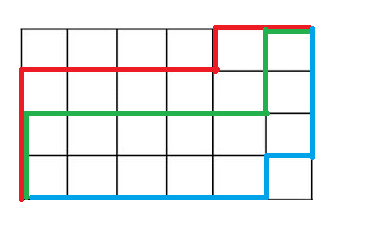
\includegraphics[width=0.66\maxwidth{\textwidth}]{recursion_grid.png}
        \end{figure}

We see that the only way to reach a cell, is to come from the left or from the bottom. So the number of ways to reach a cell is the number of ways to reach the cell to the left plus the number of ways to reach the cell on the bottom.

In other words, the number of ways to get to cell (x, y) is the sum of the ways to get to the cell (x-1, y) and the cell (x, y-1). However, the number of ways to reach the cell (x-1, y) is the sum of the number of ways to the cell (x-2, y) and (x-1, y-1). As we can see, we are solving a reduced version of the same problem! Thus we have a recurrence relation.

The base case is any cell on the left border or bottom border. There is only one way to reach the cell by either going only up or only going right.

\subsubsection{Formalization}

\begin{lstlisting}
Let path(x,y) be the number of ways to get to the grid at x and y

Base case:
paths(1,y) = 1
paths(x,1) = 1

Recurrence:
paths(x,y) = paths(x-1,y) + paths(x,y-1)

Example:
paths(3,5)
= paths(2,5) + paths(3,4)
= paths(1,5) + paths(2,4) + paths(2,4) + paths(3,3)
= 1 + paths(1,4) + paths(2,3) + paths(1,4) + paths(2,3) + paths(2,3) + paths(3,2)
= 1 + 1 + paths(1,3) + paths(2,2) + 1 + paths(1,3) + paths(2,2) + paths(1,3) + paths(2,2) + paths(2,2) + paths(3,1)
= 1 + 1 + 1 + paths(1,2) + paths(2,1) + 1 + 1 + path(1,2) + paths(2,1) + 1 + paths(1,2) + paths(2,1) + ....
= 15
\end{lstlisting}

Example of what the grid should look like

\vspace{5px}\begin{figure}[H]\centering
        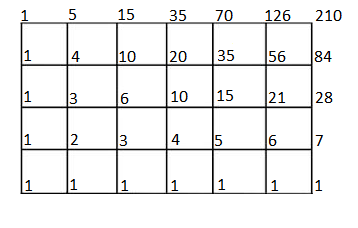
\includegraphics[width=0.66\maxwidth{\textwidth}]{recursion_grid2.png}
        \end{figure}

\subsubsection{Implementation}

\begin{lstlisting}
int paths(int n,int m){
  if (n == 1 || m == 1) {
    return 1;
  }
  return paths(n - 1, m) + paths(n, m - 1);
}
\end{lstlisting}

\subsection{Towers of Hanoi}

Suppose we have a game where there are three poles and N discs where each disc is heavier than the next disc. In the initial configuration, the discs are stacked upon another on the first pole where the lighter discs are above the heavier discs. The end goal is to move all the discs to the last pole with the following conditions:

\begin{itemize}
\item Only one disc can be moved from one pole to another at a time.
\item The discs have to be stacked such that all the lighter discs are on top of the heavier ones.
\end{itemize}

Let's try to make this problem simpler. To move N discs from the first pole the the last pole we need to move N-1 discs to the middle pole, then move the Nth disc to the last pole, and then move all N-1 discs from the middle pole back on to the last pole.

Let the starting pole be the first pole, the helper pole be the middle pole and the destination pole the third pole.

\vspace{5px}\begin{figure}[H]\centering
        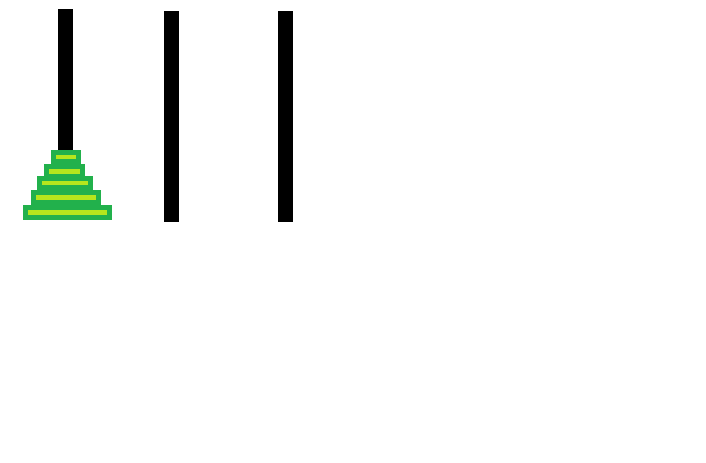
\includegraphics[width=0.66\maxwidth{\textwidth}]{hanoi.png}
        \end{figure}

To move N discs from the starting pole to the destination pole:

Step 1:

We need to move N-1 discs from the starting pole to the helper pole.
\vspace{5px}\begin{figure}[H]\centering
        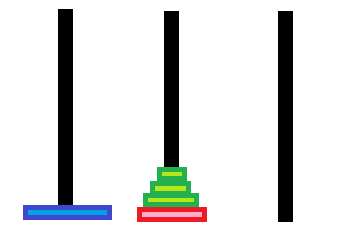
\includegraphics[width=0.66\maxwidth{\textwidth}]{hanoi2.png}
        \end{figure}

Step 2:

We need to move the Nth disc from the starting pole to the destination pole.
\vspace{5px}\begin{figure}[H]\centering
        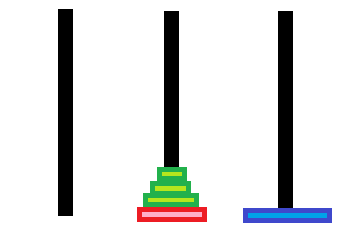
\includegraphics[width=0.66\maxwidth{\textwidth}]{hanoi3.png}
        \end{figure}

Step 3:

We need to move N-1 discs from the helper pole to the destination pole.
\vspace{5px}\begin{figure}[H]\centering
        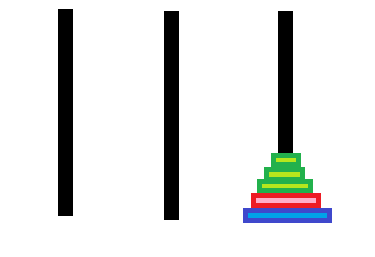
\includegraphics[width=0.66\maxwidth{\textwidth}]{hanoi4.png}
        \end{figure}

We can see that Step 2 is easy, all we have to do is move one disc. But for Step 1 and Step 3, we have to move N-1 discs. How can we move N-1 discs to the middle pole?

We see that we can use the same reasoning: we need to move N-2 discs to the third pole. Then we need to move the N-1 disc to the second pole and then move N-2 discs from the third pole to the second pole. Note that the Nth disc does not matter at all in this case since we can move any disc on top of it and we can pretend as if it doesn't exist.

In this case, the starting pole is the first pole, the helper pole is the third pole and the destination pole is the middle pole.

\vspace{5px}\begin{figure}[H]\centering
        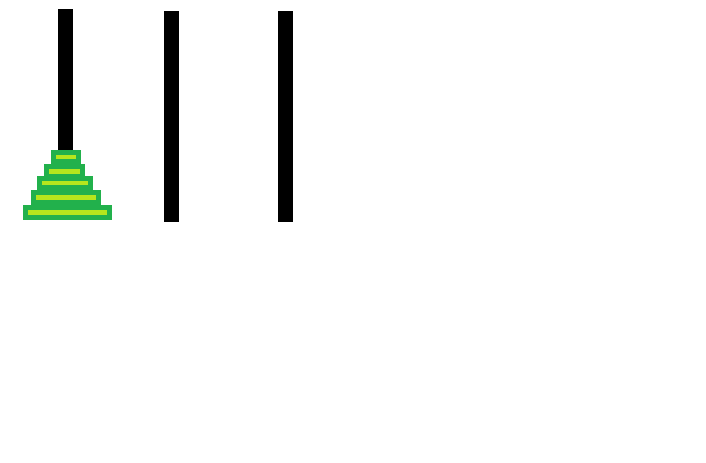
\includegraphics[width=0.66\maxwidth{\textwidth}]{hanoi.png}
        \end{figure}

To move N-1 discs from starting pole to destination pole:

Step 1:

We need to move N-2 discs from starting pole to helper pole

\vspace{5px}\begin{figure}[H]\centering
        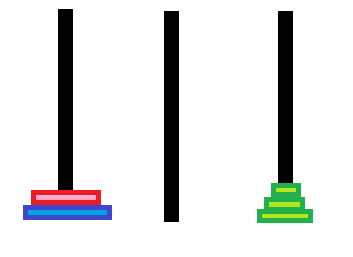
\includegraphics[width=0.66\maxwidth{\textwidth}]{hanoi5.png}
        \end{figure}

Step 2:

We move the N-1th disc from the starting pole to the destination pole

\vspace{5px}\begin{figure}[H]\centering
        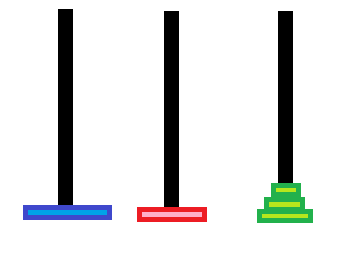
\includegraphics[width=0.66\maxwidth{\textwidth}]{hanoi6.png}
        \end{figure}

Step 3:

We move N-2 discs from the helper pole to the destination pole.

\vspace{5px}\begin{figure}[H]\centering
        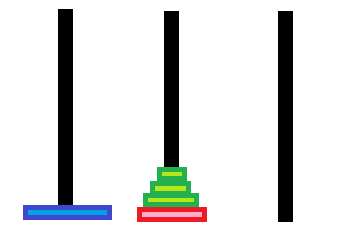
\includegraphics[width=0.66\maxwidth{\textwidth}]{hanoi2.png}
        \end{figure}

As we can see, the steps to move N discs are exactly the same as to move N-1 discs! The only difference is that the actual poles are different but the steps are the same relative to their roles (starting, helper and destination). We are solving a reduced version of the same problem, thus we have a recurrence.

In Step 1, when we move N-1 discs from start to helper, the new helper is the old destination and the new destination is the old helper.

In Step 3, when we move N-1 discs from the helper to the destination, the new helper is the start pole, and the new start pole is the helper

\subsubsection{Formalization}

\begin{lstlisting}
Let hanoi(N, start, helper, dest) print the steps to move N discs from the start to dest

Base case:
hanoi(1, start, helper, dest):
  print "Move from (start) to (dest)"

Recurrence:
hanoi(N, start, helper, dest):
  hanoi(N - 1, start, dest, helper)
  print "Move from start to dest"
  hanoi(N - 1, helper, start, dest)

Example:
Let A, B, C be pole 1, 2, 3

hanoi(4,A,B,C) 

=

hanoi(3,A,C,B)
Move from A to C
hanoi(3,B,A,C)

=

hanoi(2,A,B,C)
Move from A to B
hanoi(2,C,A,B)
Move from A to C
hanoi(2,B,A,C)
Move from B to C
hanoi(2,A,B,C)

=

hanoi(1,A,C,B)
Move from A to C
hanoi(1,B,A,C)
Move from A to B
hanoi(1,C,B,A)
Move from C to B
hanoi(1,A,C,B)
Move from A to C
hanoi(1,B,C,A)
Move from B to C
hanoi(1,A,B,C)
Move from B to C
hanoi(1,A,C,B)
Move from A to C
hanoi(1,B,A,C)

=

Move from A to B
Move from A to C
Move from B to C
Move from A to B
Move from C to A
Move from C to B
Move from A to B
Move from A to C
Move from B to A
Move from B to C
Move from A to C
Move from B to C
Move from A to B
Move from A to C
Move from B to C

\end{lstlisting}

\subsubsection{Implementation}

\begin{lstlisting}
void hanoi(int N, int start, int helper, int destination) {
  // Base case to move one disk.
  if (N == 1) {
    System.out.println("Move " + start + " to " + destination);
  }
  else {
    // Move N-1 discs from start to helper.
    hanoi(N - 1, start, destination, helper);

    // Move 1 disc from start to end.
    hanoi(1, start, helper, destination);

    // Move N-1 discs from helper to end.
    hanoi(N - 1, helper, start, destination);
  }
}
hanoi(4, 1, 2, 3);
\end{lstlisting}

\subsection{Permutations}

A permutation is an arrangement of the original set of elements.

For example, here we have a few permutations of A,B,C,D,E,F:

\begin{itemize}
\item D,E,F,C,B,A
\item F,C,D,B,A,E
\item B,D,A,E,F,C
\item A,B,C,D,E,F
\end{itemize}

Given a string S of length N, how can we generate all permutations?

Let's assume that we have a list of permutations for the substring of S of N-1 characters. To get the permutations for a string of length N, we need to insert the Nth character in between all the positions of each permutation of N-1 characters. For example, here is how the permutation of A,B,C,D is generated.

We can manually find the permutations of A,B,C.

\begin{itemize}
\item A,B,C
\item A,C,B
\item B,A,C
\item B,C,A
\item C,A,B
\item C,B,A
\end{itemize}

If we insert the letter D between each letter for every permutation in N-1 letters, we get:

\begin{itemize}
\item D,A,B,C
\item A,D,B,C
\item A,B,D,C
\item A,B,C,D
\item D,A,C,B
\item A,D,C,B
\item A,C,D,B
\item A,C,B,D
.... etc
\end{itemize}

And we can guarantee that every new permutation will be unique. (Try to prove that to yourself).

But let's look at how we can get the permutations of A,B,C. We can also get all the permutations of the string by taking the permutations of A,B and inserting C in all the positions for all substrings.

Substrings of A,B

\begin{itemize}
\item A, B
\item B, A
\end{itemize}

Insert C for all positions for all permutations

\begin{itemize}
\item C,A,B
\item A,C,B
\item A,B,C
\item C,B,A
\item B,C,A
\item C,B,A
\end{itemize}

For simplicity, S[i..j] will mean the substring from i inclusive to j exclusive. For example, if S = "abcd", S[0] = 'a' and S[1..4] = "bcd".

We see that we are solving the same reduced problem, thus we have a recurrence relation. To get the permutations of a string N, we take the string[0..N-1] and we insert the Nth character at every position for each permutation of the N-1 substring. The base case is an empty string. Permutation of an empty string is an empty list.

\begin{lstlisting}
Let permute(S) be a list of permutations for the string S

Let insertAll(ch, stringArr) be a function that inserts the character ch in every position in every string stringArr.

Example: 
insertAll('c', ['ab','ba']) = ['cab', 'acb', 'bac', 'cba', 'bca', 'bac'] 

Base case:
permute("") = [""]

Recurrence:
Let N be the length of string S
permute(S) = insertAll(S[0], permute(S[1..N]) )

Example:
permute('ABC')
= insertAll('A', permute('BC')
= insertAll('A', insertAll('B', permute('C'))
= insertAll('A', insertAll('B', insertAll('C', permute(''))))
= insertAll('A', insertAll('B', insertAll('C', [''])))
= insertAll('A', insertAll('B', ['C']))
= insertAll('A', ['BC', 'CB'])
= ['ABC', 'BAC', 'BCA', 'ACB', 'CAB', 'CBA']
\end{lstlisting}

\subsubsection{Implementation}

\begin{lstlisting}
Vector<String> insertAll(char ch, Vector<String> strArr) {
  Vector<String> vec = new Vector<String>();
  for (int i = 0; i < strArr.size(); i++) {
    String str = strArr.get(i);
    for (int j = 0; j <= str.length(); j++) {
      vec.add(str.substring(0, j) + ch + str.substring(j, str.length()));
    }
  }
  return vec;
}

Vector<String> permutation(String s) {
  int n = s.length();
  // Base case of one empty string.
  if (n == 1) {
    Vector<String> vec = new Vector<String>();
    vec.add(s.substring(0, 1));
    return vec;
  }
  // Recursive relation.
  return insertAll(s.charAt(0), permutation(s.substring(1)));
}

// Example usage:
permutation("abc");
\end{lstlisting}

\subsection{Exercises}

\begin{enumerate}
\item Given a string S, write a recursive function to generate all its non-empty substrings.
\item Write a solution for hanoi towers but with the restriction that discs can only be moved from adjacent poles. (You can move a disc from A to B but not A to C because they are not adjacent).
\item Write the formalization and code for a recursive insertAll(ch, stringArr).
\end{enumerate}

\part{ Data Structures }
    \subsubsection{ Introduction }
    

Data structures are different ways of storing data such that they optimize certain data operations such as retrieval and insertion. Although many of these data structures are already built into various languages, it is important to understand how they work. By understanding the implementations, we can have a sense of which data structure to use for different scenarios.

An abstract data type is a conceptual model for representing data. An abstract data type tells what it should do as opposed to how it should work. It will tell us what operations it should have but should not tell us how to implement them.

For example, a bottle should be able to hold water and allow us to drink from it. This tells us what it should do but we don't need to know how it works or how it is made. A plastic water bottle is an implementation of a bottle. It holds water in its interior and allows us to drink by unscrewing the cap and letting us pour water down our throat. A thermos is also an implementation of the bottle, it has a lid that can be popped open. and water can come from it. A thermos and plastic water bottle are different implementations as they are made differently and used differently, but they fundamentally do what a bottle is supposed to do: store liquid and provide a way to drink. A bottle in the abstract does not actually exist, but types of bottles do.

\vspace{5px}\begin{figure}[H]\centering
        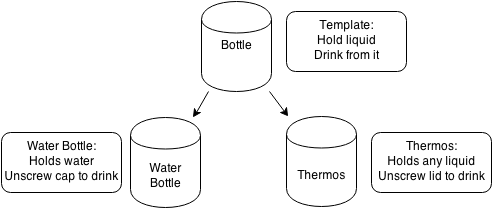
\includegraphics[width=0.66\maxwidth{\textwidth}]{bottle.png}
        \end{figure}

Some implementations of abstract data types are better than others for different purposes. For example, plastic water bottles are very cheap, whereas a thermos is more expensive. However, a thermos can hold hot water and keep it warm for a longer period of time. When selecting a data structure, we should pick one based on the efficiencies of data operations that we will do most often.

\vspace{5px}\begin{figure}[H]\centering
        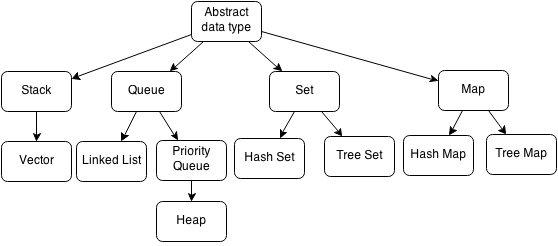
\includegraphics[width=0.66\maxwidth{\textwidth}]{adt.png}
        \end{figure}


    \chapter{ Stack }
        \section{ Stack }
        

A stack is an abstract data type with the property that it can remove and insert elements following a FILO (First In Last Out) structure. The first element to be inserted must be the last element to be removed and the last element to be inserted must be the first element to be removed. Sometimes, removal is called "pop" and insertion is called "push".

Imagine a stack of plates at a buffet, the plates are taken from the top and are also replaced from the top. The first plate to go in will be the last plate to come out. The last plate to go in will be the first to come out. This structure is what a stack is.

Example of push:

\vspace{5px}\begin{figure}[H]\centering
        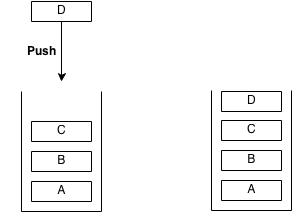
\includegraphics[width=0.66\maxwidth{\textwidth}]{stack.png}
        \end{figure}

Example of pop:

\vspace{5px}\begin{figure}[H]\centering
        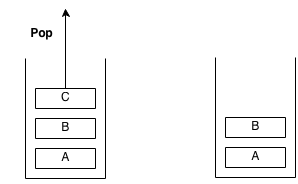
\includegraphics[width=0.66\maxwidth{\textwidth}]{stack2.png}
        \end{figure}

Stacks are used to keep track of function calls in memory. Whenever a function is called, it is placed on the memory stack with its variables, and when it is returning a value, it is popped off the stack.

A stack is usually implemented as a vector.


        

\begin{center}\begin{tabulary}{0.4\linewidth}{|l|l|l|l|l|l|l|l|l|l|l|l|l|l|l|l|l|l|l}\hline


  Implementation &
  Pop &
  Push\\
\hline


  Vector &
  O(1) &
  O(1)\\

\hline\end{tabulary}\end{center}


        \section{ Vector }
        

Prerequisites: Arrays, Stack



A vector is a stack that is implemented as an array. It is very similar to an array, but it is more flexible in terms of size. Elements are added and removed only from the end of the array. When more elements are added to the vector and the vector is at full capacity, the vector resizes itself and reallocates for 2*N space. When using an vector we can keep adding elements and let the data structure handle all the memory allocation.

\begin{center}\begin{tabulary}{0.4\linewidth}{|l|l|l|l|l|l|l|l|l|l|l|l|l|l|l|l|l|l|l}\hline


  Operation &
  Get &
  Push &
  Pop &
  Insert\\
\hline


  Time Complexity &
  O(1) &
  O(1) &
  O(1) &
  O(n)\\

\hline\end{tabulary}\end{center}

\subsection{Class}

There is a builtin Vector class already, but we will go through the implementation of a simple integer vector class to understand how the data structure works.

In our vector class, we need to store the element and the size of the current vector.

\begin{lstlisting}
public class Vec {
  private int[] arr;
  int size = 0;

  public Vec(int size) {
    arr = new int[size];
  }
}
\end{lstlisting}

\subsection{Resize}

Resize will be used to resize the array to have twice the capacity. We create a new array of two times the size of the old one and copy the old elements over.

\vspace{5px}\begin{figure}[H]\centering
        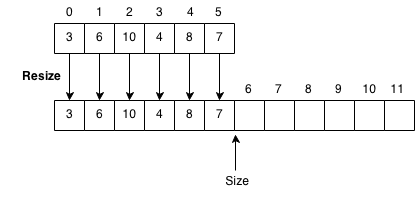
\includegraphics[width=0.66\maxwidth{\textwidth}]{vector3.png}
        \end{figure}

\begin{lstlisting}
public void resize() {
  int[] newArr = new int[2 * arr.length];
  // Copy to new array.
  for (int i = 0; i < size; i++) {
    newArr[i] = arr[i];
  }
  arr = newArr;
}
\end{lstlisting}

\subsection{Add Element}

Add element will add elements to the end of the vector. If the array is full, the vector will resize itself.

\vspace{5px}\begin{figure}[H]\centering
        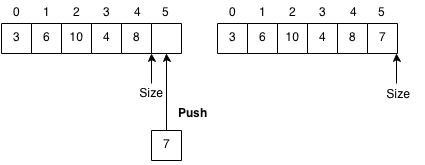
\includegraphics[width=0.66\maxwidth{\textwidth}]{vector2.png}
        \end{figure}

\begin{lstlisting}
public void add(int x) {
  if (size >= arr.length) {
    resize();
  }
  arr[size] = x;
  size++;
}
\end{lstlisting}

\subsection{Pop}

Removes the element at the end of the vector. We decrease the size of the vector and return the last element.

\vspace{5px}\begin{figure}[H]\centering
        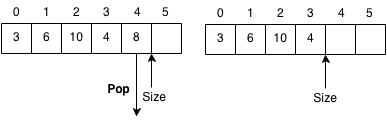
\includegraphics[width=0.66\maxwidth{\textwidth}]{vector4.png}
        \end{figure}

\begin{lstlisting}
public int pop() {
  if (size == 0) {
    throw new NoSuchElementException();
  }
  int ret = arr[size];
  size--;
  return ret;
}
\end{lstlisting}

\subsection{Remove}

Removes element at index and shifts all elements to the right of it to the left by one.

\vspace{5px}\begin{figure}[H]\centering
        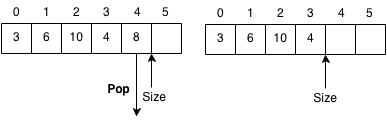
\includegraphics[width=0.66\maxwidth{\textwidth}]{vector4.png}
        \end{figure}

\begin{lstlisting}
public int remove(int idx) {
  if (idx < 0 || idx >= size) {
    throw new ArrayIndexOutOfBoundsException();
  }
  int ret = arr[idx];
  while (idx + 1 < size) {
    arr[idx] = arr[idx + 1];
    idx++;
  }
  size--;
  return ret;
}
\end{lstlisting}

\subsection{Get Element}

Returns the element at the specified index. It will throw an exception if the index is out of bounds.

\vspace{5px}\begin{figure}[H]\centering
        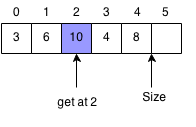
\includegraphics[width=0.66\maxwidth{\textwidth}]{vectorget.png}
        \end{figure}

\begin{lstlisting}
public int get(int idx) {
  if (idx < 0 || idx >= size) {
    throw new ArrayIndexOutOfBoundsException();
  }
  return arr[idx];
}
\end{lstlisting}

\subsection{Insert Element}

Insert the new number x at the index.

\vspace{5px}\begin{figure}[H]\centering
        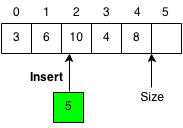
\includegraphics[width=0.66\maxwidth{\textwidth}]{vectorinsert.png}
        \end{figure}

We need to make space for the new element so when we insert the element, we have to shift all the elements to the right of the index by 1.

\vspace{5px}\begin{figure}[H]\centering
        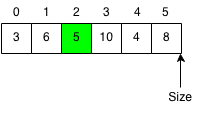
\includegraphics[width=0.66\maxwidth{\textwidth}]{vectorinsert2.png}
        \end{figure}

\begin{lstlisting}
public void insert(int idx, int x) {
  if (idx < 0 || idx > size) {
    throw new ArrayIndexOutOfBoundsException();
  }
  size++;
  if (size >= arr.length) {
    resize();
  }
  int idx2 = size;
  // Shift elements to the right.
  while (idx2 > idx) {
    arr[idx2] = arr[idx2 - 1];
    idx2--;
  }
  // Insert element.
  arr[idx] = x;
}
\end{lstlisting}

\subsection{Exercises}

\begin{enumerate}
\item Implement add(Vector v) to the Vector class, which adds all the elements of v to the current vector.
\item Implement remove(Integer i) that finds the element i and removes it from the current vector.
\end{enumerate}

        \section{ Exercises }
        

\begin{enumerate}
\item Given a string of brackets of either () or [], determine if the bracket syntax is legal (every opening bracket has a closing bracket from left to right).

Legal syntax:

\begin{itemize}
\item ( [ ( ) [ ] ] )
\item ( ) ( ) [ ] ( ) ( )
\end{itemize}

Illegal syntax:

\begin{itemize}
\item ( ( ) ]
\item ( ) [ ( ] )
\end{itemize}
\end{enumerate}

    \chapter{ Queue }
        \section{ Queue }
        

A queue is an abstract data type with two functions, pop and push. Removal from the front is called "pop" or "dequeue". Insertion from the back is called "push" or "enqueue". A queue follows a First In First Out (FIFO) structure meaning the first element pushed should be the first element popped and the last element pushed should be the last element popped.

Imagine you are standing in line for a restaurant. Whoever is first in line will be served first and whoever is last in line will be served last. People can be served while more people join the line and the line may get very long because it takes a while to serve one person while more people join the queue. This is called a queue.

Queues are often used for buffer systems, such as a text message service. The messages that arrive at the server first are relayed first and the messages that arrive later are relayed later. If there are too many text messages in the system such that the rate  texts are received overwhelm the number of texts that are sent the buffer may overflow and messages will get dropped. Most of the time this won't happen because the systems are designed to handle large loads, but if there were an emergency that caused everyone to start texting many texts could be dropped.

Example of push:

\vspace{5px}\begin{figure}[H]\centering
        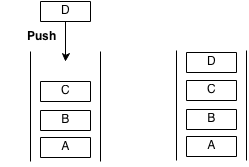
\includegraphics[width=0.66\maxwidth{\textwidth}]{queue.png}
        \end{figure}

Example of pop:

\vspace{5px}\begin{figure}[H]\centering
        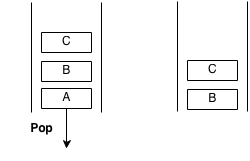
\includegraphics[width=0.66\maxwidth{\textwidth}]{queue2.png}
        \end{figure}


        

We can implement a queue most efficiently using a linked list because it uses efficient memory allocation.

\begin{center}\begin{tabulary}{0.4\linewidth}{|l|l|l|l|l|l|l|l|l|l|l|l|l|l|l|l|l|l|l}\hline


  Implementation &
  Pop &
  Push\\
\hline


  Linked List &
  O(1) &
  O(1)\\

\hline\end{tabulary}\end{center}


        \section{ Linked List }
        

Prerequisites: Queue



A linked list is an implementation of a queue that uses a chain of pointers. Instead of storing all the data in a fixed set of memory, we can store each element by itself but have a pointer from each element to the next element. A pointer is something that holds the memory location of another object.

Imagine you were on a scavenger hunt with lots of treasure chests. You start with a clue to the first chest. Each chest contains a lot of gold (data) but it also contains a clue to the next treasure chest. To get to the fifth chest, you need to visit the first, second, third and fourth chest. This is essentially how a linked list works.

\vspace{5px}\begin{figure}[H]\centering
        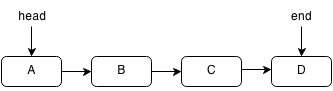
\includegraphics[width=0.66\maxwidth{\textwidth}]{linkedlist.png}
        \end{figure}

A linked list is similar to an array but it is different such that it is not stored in one block of data. Each element can be stored in a random place in memory but each element contains a pointer to the next element thus forming a chain of pointers. Think of a pointer as a clue to the next chest. Since the elements aren't in a block, accessing an element must be done by traversing the entire linked list by following each pointer to the next. However, this also allows insertion and deletion to be done more quickly. In a linked list the links only go forward and you cannot move backward. However, a doubly linked list is a linked list that has pointers going backwards as well as forwards.

\vspace{5px}\begin{figure}[H]\centering
        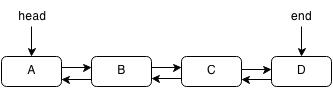
\includegraphics[width=0.66\maxwidth{\textwidth}]{doublelinkedlist.png}
        \end{figure}

\begin{center}\begin{tabulary}{0.4\linewidth}{|l|l|l|l|l|l|l|l|l|l|l|l|l|l|l|l|l|l|l}\hline


  Operation &
  Get &
  Push &
  Delete &
  Insert\\
\hline


  Time Complexity &
  O(n) &
  O(1) &
  O(1) &
  O(1)\\

\hline\end{tabulary}\end{center}

\subsection{Link Class}

In Java, there already exists a LinkedList class but we will implement our own.

We need a Link class for each "link" in the Linked List. In each Link we only need the value and location of the previous and next node.

\begin{lstlisting}
class Link {
  int value;
  Link next;

  public Link(int value) {
    this.value = value;
    this.next = null;
  }
}
\end{lstlisting}

\subsection{LinkedList Class}

Create the linked list by initializing the starting node and ending node as null and setting the size to empty.

\begin{lstlisting}
public class LinkedList {

  public Link head;
  public Link end;
  public int size;

  public LinkedList() {
    head = null;
    end = null;
    size = 0;
  }
}
\end{lstlisting}

\subsection{Push}

Create a new node with the value given and add it to the end. We have to set the current head previous node to the new node and the new next next to the last node.

For example, if we want to insert E into the following linked list:

\vspace{5px}\begin{figure}[H]\centering
        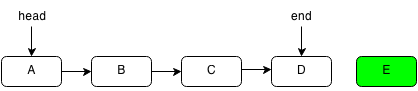
\includegraphics[width=0.66\maxwidth{\textwidth}]{linkedlistpush.png}
        \end{figure}

First, we set the next pointer of the last element to the next element.

\vspace{5px}\begin{figure}[H]\centering
        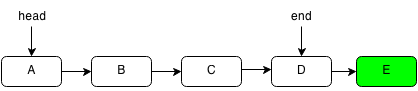
\includegraphics[width=0.66\maxwidth{\textwidth}]{linkedlistpush2.png}
        \end{figure}

Then we set the new end of the linked list.

\vspace{5px}\begin{figure}[H]\centering
        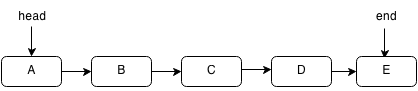
\includegraphics[width=0.66\maxwidth{\textwidth}]{linkedlistpush3.png}
        \end{figure}

\begin{lstlisting}
public void push(int value) {
  Link newLink = new Link(value);
  if (size == 0) {
    head = end = newLink;
  }
  else {
    end.next = newLink;
    end = newLink;
  }
  size++;
}
\end{lstlisting}

\subsection{Pop}

Pops off the head of the linked list and throws an exception if the linked list is empty.

For example, if we want to pop the first element of the following linked list:

\vspace{5px}\begin{figure}[H]\centering
        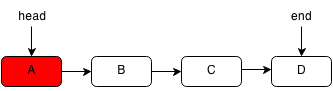
\includegraphics[width=0.66\maxwidth{\textwidth}]{linkedlistpop.png}
        \end{figure}

We set the head of the linked list to the second element.

\vspace{5px}\begin{figure}[H]\centering
        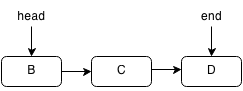
\includegraphics[width=0.66\maxwidth{\textwidth}]{linkedlistpop2.png}
        \end{figure}

\begin{lstlisting}
public int pop() {
  if (head == null) {
    throw new NoSuchElementException();
  }
  int ret = head.value;
  head = head.next;
  size--;
  if (size == 0) {
    end = null;
  }
  return ret;
}
\end{lstlisting}

\subsection{Get}

Get retrieves the value at the specified index. We have to loop through the entire list to get to the index we want.

For example, if we want to get the element C in the following linked list:

We first start at the head element and iterate through each node.

\vspace{5px}\begin{figure}[H]\centering
        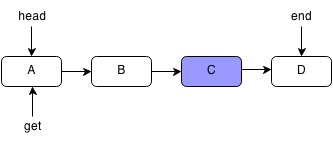
\includegraphics[width=0.66\maxwidth{\textwidth}]{linkedlistget.png}
        \end{figure}

We keep following the next pointers until we reach the node we want or the end of the linked list.

\vspace{5px}\begin{figure}[H]\centering
        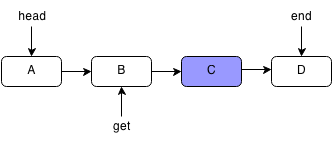
\includegraphics[width=0.66\maxwidth{\textwidth}]{linkedlistget2.png}
        \end{figure}

Since our current pointer points to C, we stop.

\vspace{5px}\begin{figure}[H]\centering
        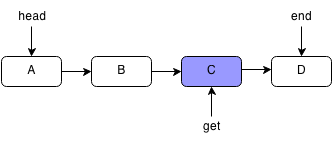
\includegraphics[width=0.66\maxwidth{\textwidth}]{linkedlistget3.png}
        \end{figure}

\begin{lstlisting}
public int get(int index) {
  int i = 0;
  Link curNode = head;
  while (curNode != null) {
    if (index == i) {
      return curNode.value;
    }
    curNode = curNode.next;
    i++;
  }
  throw new NoSuchElementException();
}
\end{lstlisting}

\subsection{Delete}

To delete the current node we set the previous node next link to the link that is next.

For example, if we wanted to delete B from the following linked list:

\vspace{5px}\begin{figure}[H]\centering
        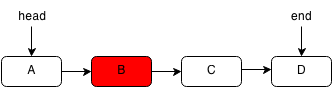
\includegraphics[width=0.66\maxwidth{\textwidth}]{linkedlistrem.png}
        \end{figure}

We would find B and set the previous node's next to B's next which is C.

\vspace{5px}\begin{figure}[H]\centering
        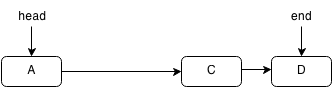
\includegraphics[width=0.66\maxwidth{\textwidth}]{linkedlistrem2.png}
        \end{figure}

\begin{lstlisting}
public void deleteNext(Link node) {
  if (node.next == end) {
    end = node;
  }
  node.next = node.next.next;
  size--;
}
\end{lstlisting}

\subsection{Exercises}

\begin{enumerate}
\item Implement a doubly linked list.
\item A game is played by always eliminating the kth player from the last elimination and played until one player is left. Given N players where each is assigned to a number, find the number of the last remaining player.

For example, you have 5 players (1,2,3,4,5) and the 3rd player is eliminated.

\begin{itemize}
\item 1, 2, 3, 4, 5 
\item 1, 2, 4, 5 (1, 2, 3 is eliminated)
\item 2, 4, 5 (4, 5, 1 is eliminated)
\item 2, 4 (2, 4, 5 is eliminated)
\item 2 (2, 4, 2 is eliminated)
\item Player 2 is the last one standing.
\end{itemize}
\item Given two linked lists which may share tails, determine the point at which they converge. For example, if our first linked list is [1,2,4,5] and our second linked list is [0,3,4,5] and each number is a node, then the two linked lists converge at 4. 
\vspace{5px}\begin{figure}[H]\centering
        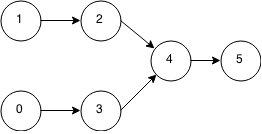
\includegraphics[width=0.66\maxwidth{\textwidth}]{linkedlistconverge.png}
        \end{figure}
\item Given a node in a doubly linked list, write a function that removes the node from the list. 
\end{enumerate}

        \section{ Exercises }
        

\begin{enumerate}
\item Given a list of letters representing instructions where the first instruction is executed, output what the final list should look like after N instructions are executed.

First instruction:

\begin{itemize}
\item A. Add B to the end of the list of instructions
\item B. Do nothing
\item C. Add two A's to the front of the list of instructions
\end{itemize}

Example:

\begin{itemize}
\item ABC
\item BCB
\item CB
\item AAB
\item ABB
\item BBB
\item BB
\item B
\end{itemize}
\end{enumerate}

    \chapter{ Sets }
        \section{ Sets }
        

Sets are abstract data structures which are able to store and keep track of unique values.

Imagine you have a grocery list that you use to keep tracking of things you need to buy. You want to make sure there are no duplicate items in the list, you can add items to the list and that you can remove items from your list. This structure is similar to what a set does.

Sets have three operations: insertion, deletion and a membership test. Insertion places an element into the set, deletion removes an element from the set and a membership test is checking whether an element exists within the set.


        

\begin{center}\begin{tabulary}{0.4\linewidth}{|l|l|l|l|l|l|l|l|l|l|l|l|l|l|l|l|l|l|l}\hline


  Type &
  Membership &
  Insertion &
  Deletion\\
\hline


  Hash Set &
  O(1) &
  O(1) &
  O(1)\\

  Tree Set &
  O(log n) &
  O(log n) &
  O(log n)\\

\hline\end{tabulary}\end{center}


        \section{ Hash Set }
        

Prerequisites: Sets, Linked List



Hash sets are sets that use hashes to store elements. A hashing algorithm is an algorithm that takes an element and converts it to a chunk of a fixed size called a hash. For example, let our hashing algorithm be (x mod 10). So the hashes of 232, 217 and 19 are 2,7, and 9 respectively.

\vspace{5px}\begin{figure}[H]\centering
        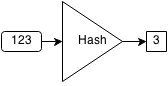
\includegraphics[width=0.66\maxwidth{\textwidth}]{hashcode.png}
        \end{figure}

For every element in a hash set, the hash is computed and elements with the same hash are grouped together. This group of similar hashes is called a bucket and they are usually stored as linked lists.

If we want to check if an element already exists within the set, we first compute the hash of the element and then search through the bucket associated with the hash to see if the element is contained.

\vspace{5px}\begin{figure}[H]\centering
        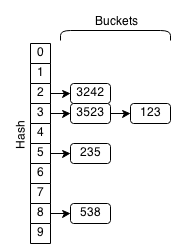
\includegraphics[width=0.66\maxwidth{\textwidth}]{hashset.png}
        \end{figure}

\begin{center}\begin{tabulary}{0.4\linewidth}{|l|l|l|l|l|l|l|l|l|l|l|l|l|l|l|l|l|l|l}\hline


  Operation &
  Membership &
  Insertion &
  Deletion\\
\hline


  Time Complexity &
  O(1) &
  O(1) &
  O(1)\\

\hline\end{tabulary}\end{center}

\subsection{Class}

Inside our implementation of a hash set, we will store the buckets (using an array of linked lists), the number of buckets, and the number of elements in the set.

The collision chance is the threshold for resizing the hash set. When the ratio of elements in the set to number of buckets is greater than the threshold, then the chance of collision will be high enough that it will slow down the operations. The lower this ratio, the better performing a hash set will be.

\begin{lstlisting}
public class HashSet {

  public LinkedList<Integer>[] buckets;
  public int bucketsSize = 10;
  public int size = 0;
  public static final double COLLISION_CHANCE = 0.3;

  public HashSet() {
    // Create buckets.
    buckets = new LinkedList[10];
    for (int i = 0; i < bucketsSize; i++) {
      buckets[i] = new LinkedList<Integer>();
    }
    size = 0;
  }
}
\end{lstlisting}

If we wanted to check if 7238 was in the hash set, we would get the hash (7238 mod 10 = 8). So we get the bucket associated with the hash 8 and we get the list of [538]. When we iterate through this short list, we see that 7238 is not a member of the set.

Similarly, if we wanted to insert 7238 into the hash set, we would check if it exists and if it did not, we would add the element to the bucket. For deletion, we would find 7238 and then remove it from the bucket if it existed.

Hash sets are very efficient in all three set operations if a good hashing algorithm is used. When the objects are that being stored are large then hash sets are effective as a set.

\subsection{Hash code}

The hash code is the result of the hashing algorithm for an element. In our hash set implementation, we will use a simple hash: modulus of the integer by the number of buckets.

\vspace{5px}\begin{figure}[H]\centering
        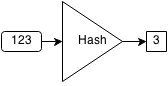
\includegraphics[width=0.66\maxwidth{\textwidth}]{hashcode.png}
        \end{figure}

For the most part, if the numbers are all random, then the hash function will perform well. However, if the number of buckets was 10 and we added the elements 20,30,40,50,60,70, then they would all end up in the same bucket and performance degenerates to a linked list. A good hash function can prevent this from occurring.

\begin{lstlisting}
public int getHash(int x, int hashSize) {
  // Use modulus as hash function.
  return x % hashSize;
}
\end{lstlisting}

\subsection{Resize}

A hash set must be able to resize. When the ratio of number of elements to number of buckets, the chance of collision will increase more and more. So we must able to resize the number of buckets to support the number of elements to lower the chance of collision.

To resize efficiently, we can create two times the number of buckets and set them to empty and then insert all the elements in the old buckets to the new buckets.

\begin{lstlisting}
public void resize() {
  // Double number of buckets.
  int newBucketsSize = bucketsSize * 2;
  LinkedList<Integer>[] newBuckets = new LinkedList[newBucketsSize];
  
  // Create new buckets.
  for (int i = 0; i < newBucketsSize; i++) {
    newBuckets[i] = new LinkedList<Integer>();
  }
  
  // Copy elements over and use new hashes.
  for (int i = 0; i < bucketsSize; i++) {
    for (Integer y : buckets[i]) {
      int hash = getHash(y, newBucketsSize);
      newBuckets[hash].push(y);
    }
  }
  
  // Set new buckets.
  buckets = newBuckets;
  bucketsSize = newBucketsSize;
}
\end{lstlisting}

\subsection{Insert}

To insert an element in a hash set, we get the hash code from our hashing algorithm and insert the element into the corresponding bucket.

For example, if we want to insert 88 in the following hash set:

\vspace{5px}\begin{figure}[H]\centering
        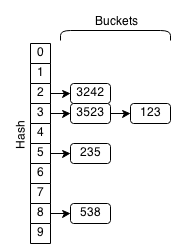
\includegraphics[width=0.66\maxwidth{\textwidth}]{hashset.png}
        \end{figure}

We compute the hash of 88 which is 8, and we insert it to the end of the bucket with hash 8.

\vspace{5px}\begin{figure}[H]\centering
        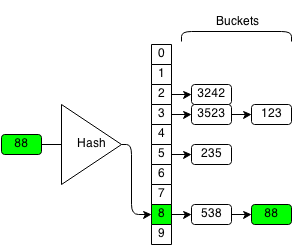
\includegraphics[width=0.66\maxwidth{\textwidth}]{hashsetinsert.png}
        \end{figure}

The function will return whether or not the operation was successful. If the bucket already contains the element, the operation will stop because we do not want to add duplicate elements into the set. If the bucket does not contain the element, we will insert it into the bucket and the operation is successful.

\begin{lstlisting}
public boolean insert(int x) {
  // Get hash of x.
  int hash = getHash(x, bucketsSize);

  // Get current bucket from hash.
  LinkedList<Integer> curBucket = buckets[hash];
  
  // Stop, if current bucket already has x.
  if (curBucket.contains(x)) {
    return false;
  }
  
  // Otherwise, add x to the bucket.
  curBucket.push(x);
  
  // Resize if the collision chance is higher than threshold.
  if ((float) size / bucketsSize > COLLISION_CHANCE) {
    resize();
  }
  size++;
  return true;
}
\end{lstlisting}

\subsection{Contains}

To check if a hash set contains an element, we get the hash code from our hashing algorithm and check if the corresponding bucket contains the element.

For example, if want to check if 123 is in the hash set:

We compute the hash of 123 which is 3 and search the bucket with hash 3.

\vspace{5px}\begin{figure}[H]\centering
        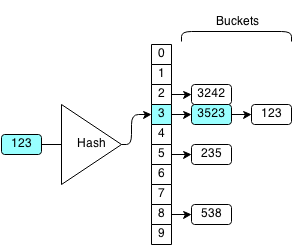
\includegraphics[width=0.66\maxwidth{\textwidth}]{hashsetcontains.png}
        \end{figure}

We iterate through the bucket until we find the element we want and return true. Otherwise, if we cannot find the element in the bucket we return false.

\vspace{5px}\begin{figure}[H]\centering
        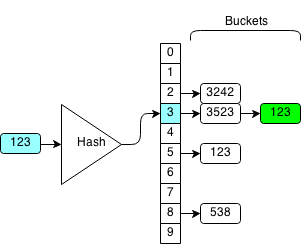
\includegraphics[width=0.66\maxwidth{\textwidth}]{hashsetcontains3.png}
        \end{figure}

\begin{lstlisting}
public boolean contains(int x) {
  // Get hash of x.
  int hash = getHash(x, bucketsSize);
  
  // Get current bucket from hash.
  LinkedList<Integer> curBucket = buckets[hash];
  
  // Return if bucket contains x.
  return curBucket.contains(x);
}
\end{lstlisting}

\subsection{Remove}

To remove an element from a hash set, we get the hash code from our hashing algorithm and remove the element from the corresponding bucket.

The function will return whether or not the operation was successful. If the bucket contains the element we can remove it from the linked list and the operation is successful. If the element is not in the bucket then the operation fails because we cannot remove something that is not there.

For example, we want to remove 123 from the hash set:

We compute the hash of 123 which is 3 and we search the bucket with hash 3.

\vspace{5px}\begin{figure}[H]\centering
        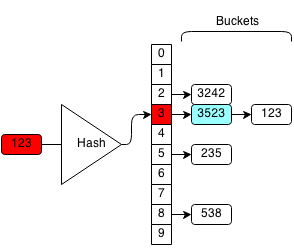
\includegraphics[width=0.66\maxwidth{\textwidth}]{hashsetrem.png}
        \end{figure}

We iterate through each element in the bucket until we find 123.

\vspace{5px}\begin{figure}[H]\centering
        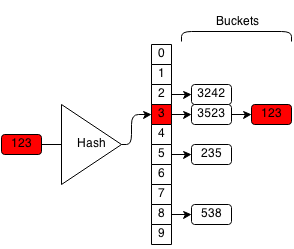
\includegraphics[width=0.66\maxwidth{\textwidth}]{hashsetrem2.png}
        \end{figure}

If we find the element, we delete the element from the bucket.

\vspace{5px}\begin{figure}[H]\centering
        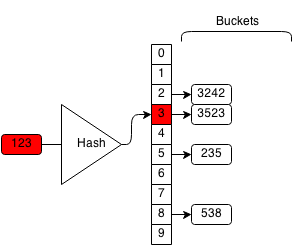
\includegraphics[width=0.66\maxwidth{\textwidth}]{hashsetrem3.png}
        \end{figure}

\begin{lstlisting}
public boolean remove(int x) {
  // Get hash of x.
  int hash = getHash(x, bucketsSize);
  
  // Get bucket from hash.
  LinkedList<Integer> curBucket = buckets[hash];
  
  // Remove x from bucket and return if operation successful.
  return curBucket.remove((Integer) x);
}
\end{lstlisting}

\subsection{Exercises}

\begin{enumerate}
\item Devise a hashing algorithm for strings.
\item Calculate the probability of a collision occurring given the number of buckets and number of elements in the hash set.
\item Prove that the runtime of all the operations are O(1).
\end{enumerate}

        \section{ Tree Set }
        

Prerequeisites: Sets, Binary Search Tree



A tree set is a set which stores the values in a binary search tree. To store elements in a tree set, they must be able to be sorted by a property. To insert an element, it is added to the binary tree. To delete an element, it is removed from the binary tree. To check for membership, we do a binary search for the element in the binary tree.

The advantage of tree sets is that they are maintained in a sorted order.

Tree Sets are implemented using binary search trees.

\vspace{5px}\begin{figure}[H]\centering
        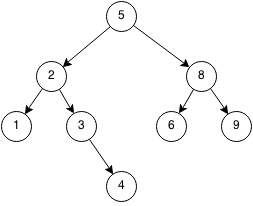
\includegraphics[width=0.66\maxwidth{\textwidth}]{bst.png}
        \end{figure}


        

\begin{center}\begin{tabulary}{0.4\linewidth}{|l|l|l|l|l|l|l|l|l|l|l|l|l|l|l|l|l|l|l}\hline


  Operation &
  Membership &
  Insertion &
  Deletion\\
\hline


  Binary Search Tree &
  O(log n) &
  O(log n) &
  O(log n)\\

\hline\end{tabulary}\end{center}


        \section{ Binary Search Tree }
        

Prerequisites: Set, Binary Tree

A binary search tree is a  binary tree with special properties. For every node in the tree, the values of all the nodes in left subtree of a node will always be less than the value of the node and all the nodes in the right subtree will always be more than the value of the node. It has a recursive structure meaning every subtree is also a binary search tree.

Structure:

\vspace{5px}\begin{figure}[H]\centering
        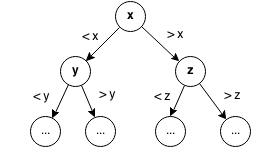
\includegraphics[width=0.66\maxwidth{\textwidth}]{bstcompare.png}
        \end{figure}

Example:

\vspace{5px}\begin{figure}[H]\centering
        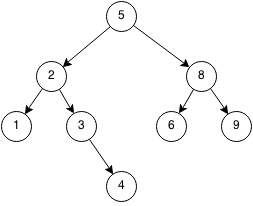
\includegraphics[width=0.66\maxwidth{\textwidth}]{bst.png}
        \end{figure}

\begin{center}\begin{tabulary}{0.4\linewidth}{|l|l|l|l|l|l|l|l|l|l|l|l|l|l|l|l|l|l|l}\hline


  Operation &
  Membership &
  Insertion &
  Deletion\\
\hline


  Time Complexity &
  O(log n) &
  O(log n) &
  O(log n)\\

\hline\end{tabulary}\end{center}

\subsection{Class}

In a binary search tree, everything to the left of a node is smaller than that node and everything to the right of that node is greater than that node.

Structure:

\vspace{5px}\begin{figure}[H]\centering
        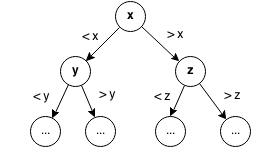
\includegraphics[width=0.66\maxwidth{\textwidth}]{bstcompare.png}
        \end{figure}

Example:

\vspace{5px}\begin{figure}[H]\centering
        \includegraphics[width=0.66\maxwidth{\textwidth}]{bst.png}
        \end{figure}

\subsubsection{Implementation}

A Node is a node in our binary search tree. Each node will contain a left subtree, a right subtree, the parent of the tree and the value stored at that node. It is unnecessary to store the parent, but for this implementation it will be easier to keep track of the parent.

replaceChild replaces the left or right child node specified with the replacement node.

\begin{lstlisting}
public class Node {
  int value;
  Node left;
  Node right;
  Node parent;

  public Node(int val, Node parent) {
    this.value = val;
    this.left = null;
    this.right = null;
    this.parent = parent;
  }

  // Replaces the child node with the replacement one.
  public void replaceChild(Node child, Node replacement) {
    // If replacing left child.
    if (left == child) {
      left = replacement;
    }
    // If replacing right child.
    if (right == child) {
      right = replacement;
    }
    // Set replacement nodes parent.
    if (replacement != null) {
      replacement.parent = this;
    }
  }
}
\end{lstlisting}

In our class we will store the number of element in the set and the root of the tree. From the root of the tree we can traverse the rest of the tree.

\begin{lstlisting}
public class BinarySearchTree {
  int size;
  Node root;
    
  public BinarySearchTree(){
    size = 0;
    root = null;
  }
}
\end{lstlisting}

\subsection{Insert}

To insert an element in the tree set we search for the element that we are trying to insert. If it is already there then the operation fails because sets contain unique elements. Otherwise we will insert the new element into the set.

Let's insert 4 into the binary search tree. We first start at the root at 5.

\vspace{5px}\begin{figure}[H]\centering
        \includegraphics[width=0.66\maxwidth{\textwidth}]{bstinsert.png}
        \end{figure}

Since 4 is less than 5, we traverse the left subtree to 2.

\vspace{5px}\begin{figure}[H]\centering
        \includegraphics[width=0.66\maxwidth{\textwidth}]{bstinsert2.png}
        \end{figure}

Since 4 is greater than 2, we traverse the right subtree to 3.

\vspace{5px}\begin{figure}[H]\centering
        \includegraphics[width=0.66\maxwidth{\textwidth}]{bstinsert3.png}
        \end{figure}

Since 4 is greater than 3 and there is no right child, than we create a new node with the value 4 as the right child.

\vspace{5px}\begin{figure}[H]\centering
        \includegraphics[width=0.66\maxwidth{\textwidth}]{bstinsert4.png}
        \end{figure}

\subsubsection{Implementation}

\begin{lstlisting}
public boolean insert(int x) {
  // If root is missing.
  if (root == null) {
    root = new Node(x, null);
    size = 1;
    return true;
  }
  Node curTree = root;
  while (curTree != null) {
    // Return if x already exists in set.
    if (x == curTree.value) {
      return false;
    }
    // Traverse left if x is less than current node.
    else if (x < curTree.value) {
      // If left child is empty, create new node.
      if (curTree.left == null) {
        curTree.left = new Node(x, curTree);
        size++;
        return true;
      }
      // Traverse left child.
      curTree = curTree.left;
    }
    // Traverse right otherwise.
    else {
      // If right child is empty, create new node.
      if (curTree.right == null) {
        curTree.right = new Node(x, curTree);
        size++;
        return true;
      }
      // Traverse right child.
      curTree = curTree.right;
    }
  }
  return false;
}
\end{lstlisting}

\subsection{Contains}

To check if the tree set contains an element, we search for it in the binary tree by starting at the root. If the number is less than the current, we search the left subtree. If the number is greater than the current, we search the right subtree.

We want to check if the number 6 is in the binary search tree.

\vspace{5px}\begin{figure}[H]\centering
        \includegraphics[width=0.66\maxwidth{\textwidth}]{bstcontains.png}
        \end{figure}

Since 6 is larger than 5, we traverse the right subtree of 5.

\vspace{5px}\begin{figure}[H]\centering
        \includegraphics[width=0.66\maxwidth{\textwidth}]{bstcontains2.png}
        \end{figure}

Since 6 is less than 8, we traverse the left subtree of 8.

\vspace{5px}\begin{figure}[H]\centering
        \includegraphics[width=0.66\maxwidth{\textwidth}]{bstcontains3.png}
        \end{figure}

The root of the left subtree is 6, thus we have found the element. If we were to keep traversing and reach a leaf node that was not the element, then the element would not exist in the binary search tree.

\vspace{5px}\begin{figure}[H]\centering
        \includegraphics[width=0.66\maxwidth{\textwidth}]{bstcontains4.png}
        \end{figure}

\subsubsection{Implementation}

\begin{lstlisting}
public boolean contains(int x) {
  Node curTree = root;
  // Iterate through tree.
  while (curTree != null) {
    // If found element return true.
    if (x == curTree.value) {
      return true;
    }
    // Traverse left tree if x is less than current node.
    else if (x < curTree.value) {
      curTree = curTree.left;
    }
    // Traverse right tree if x is greater then current node.
    else {
      curTree = curTree.right;
    }
  }
  // Return false if not found.
  return false;
}
\end{lstlisting}

\subsection{Remove}

Removing an element is a much more complex because we need to maintain the tree structure of the tree set when removing elements. First, we locate the element that we want to remove. If the element is not there, then the operation failed and we return false. If the element is there, then are three cases we need to consider.

\vspace{5px}\begin{figure}[H]\centering
        \includegraphics[width=0.66\maxwidth{\textwidth}]{bst-rem.png}
        \end{figure}

Case 1: Node is a leaf node

\vspace{5px}\begin{figure}[H]\centering
        \includegraphics[width=0.66\maxwidth{\textwidth}]{bst-rem-case11.png}
        \end{figure}

If the node we want to remove is the leaf node, we can simply remove it.

\vspace{5px}\begin{figure}[H]\centering
        \includegraphics[width=0.66\maxwidth{\textwidth}]{bst-rem-case12.png}
        \end{figure}

Case 2: Node has one child

\vspace{5px}\begin{figure}[H]\centering
        \includegraphics[width=0.66\maxwidth{\textwidth}]{bst-rem-case21.png}
        \end{figure}

If the node we want to remove has a child, we can replace that node with its' only child.

\vspace{5px}\begin{figure}[H]\centering
        \includegraphics[width=0.66\maxwidth{\textwidth}]{bst-rem-case22.png}
        \end{figure}

Case 3: Node has two children

\vspace{5px}\begin{figure}[H]\centering
        \includegraphics[width=0.66\maxwidth{\textwidth}]{bst-rem-case31.png}
        \end{figure}

We need to replace the node with the rightmost of the left subtree or the leftmost of the right subtree to maintain the order.

\vspace{5px}\begin{figure}[H]\centering
        \includegraphics[width=0.66\maxwidth{\textwidth}]{bst-rem-case32.png}
        \end{figure}

It does not matter which side we pick, so we will use the rightmost of the left subtree. First, we copy the value of the rightmost of the left subtree into the node that will be deleted.

\vspace{5px}\begin{figure}[H]\centering
        \includegraphics[width=0.66\maxwidth{\textwidth}]{bst-rem-case33.png}
        \end{figure}

Then we replace the rightmost of the left subtree with its left subtree.

\vspace{5px}\begin{figure}[H]\centering
        \includegraphics[width=0.66\maxwidth{\textwidth}]{bst-rem-case34.png}
        \end{figure}

\subsubsection{Implementation}

\begin{lstlisting}
public boolean remove(int x) {
  // Node to be removed.
  Node curNode = root;

  // Traverse through binary tree.
  while (curNode != null) {
    // If found element, use node.
    if (x == curNode.value) {
      break;
    }
    // Traverse through left child.
    else if (x < curNode.value) {
      curNode = curNode.left;
    }
    // Traverse through right child.
    else {
      curNode = curNode.right;
    }
  }
  // If node was not found, return false.
  if (curNode == null) {
    return false;
  }
  // Case 1: Removed node has no children.
  if (curNode.left == null && curNode.right == null) {
    // Special case if root.
    if (curNode == root) {
      this.root = null;
    }
    // Replace node with null.
    else {
      curNode.parent.replaceChild(curNode, null);
    }
  }
  // Case 2a: Removed node only has a right child.
  else if (curNode.left == null) {
    // Special case if node is root.
    if (curNode == root) {
      root = curNode.right;
      root.parent = null;
    }
    // Replace current node with right child.
    else {
      curNode.parent.replaceChild(curNode, curNode.right);
    }
  }
  // Case 2b: Removed node only has a left child.
  else if (curNode.right == null) {
    // Special case if node is root.
    if (curNode == root) {
      root = curNode.left;
      root.parent = null;
    }
    // Replace current node with left child.
    else {
      curNode.parent.replaceChild(curNode, curNode.left);
    }
  }
  // Case 3: Removed node has two children.
  else {
    // Get rightmost of left subtree.
    Node rightmost = curNode.left;
    while (rightmost.right != null) {
      rightmost = rightmost.right;
    }
    // Copy rightmost of left subtree to removed node's.
    curNode.value = rightmost.value;
    // Replace rightmost of left subtree with left child.
    rightmost.parent.replaceChild(rightmost, rightmost.left);
  }
  size--;
  return true;
}
\end{lstlisting}

\subsection{Print Tree}

In a binary search tree, we can print the elements in order.

\subsubsection{Implementation}

\begin{lstlisting}
public String dfs(Node curTree) {
  if (curTree == null) {
    return "";
  }
  String ret = "";
  // Print left child.
  ret += dfs(curTree.left);
  // Print current node.
  ret += curTree.value;
  ret += ",";
  // Print right child.
  ret += dfs(curTree.right);
  return ret;
}
    
public String toString() {
  String ret = "";
  if (root != null) {
    ret += dfs(root);
  }
  return ret.substring(0, ret.length() - 1);
}
\end{lstlisting}

\subsection{Exercises}

\begin{enumerate}
\item Write a function to determine if a binary tree is a binary search tree.
\end{enumerate}

        \section{ Exercises }
        

\begin{enumerate}
\item Given a list of words, determine how many of them are anagrams of each other. An anagram is a word that can have its letters scrambled into another word. 

\begin{itemize}
\item For example, silent and listen are anagrams but banana and orange are not.
\end{itemize}
\item Given the friend lists of two people, find the number of mutual friends.
\item Given an array of numbers, find the number of pairs of numbers that sum to 0.
\item Given an array of numbers, find the number of tuples of size 4 that add to A.

\begin{itemize}
\item For example in the list (10,5,-1, 3, 4, -6) the tuple of size 4 (-1,3,4-6) adds to 0.
\end{itemize}
\end{enumerate}

    \chapter{ Maps }
        \section{ Maps }
        

Prerequisites: Sets

A map is an abstract data type that stores key-value pairs.

Imagine you had a English dictionary. If you look up a word, you can find it's definition. For example if you looked up the word 'cat' in the English dictionary, you would look through the dictionary alphabetically until you found the word 'cat' and then you would look at the definition: 'a feline animal'. If you really wanted to, you could also add your own words into the dictionary and the definitions of your words. This type of structure is called a map.

Maps (also called dictionaries) are abstract data types that store pairs of key-values and can be used to look up values from the keys. The keys are like the words in an English dictionary and the definitions can be seen as the values. Maps are able to insert key-value pairs, retrieve values from keys, and delete key-value pairs.


        

\begin{center}\begin{tabulary}{0.4\linewidth}{|l|l|l|l|l|l|l|l|l|l|l|l|l|l|l|l|l|l|l}\hline


  Type &
  Get &
  Put &
  Deletion\\
\hline


  Hash Map &
  O(1) &
  O(1) &
  O(1)\\

  Tree Map &
  O(log n) &
  O(log n) &
  O(log n)\\

\hline\end{tabulary}\end{center}


        \section{ Hash Map }
        

Prerequisites: Map, Hash Set



Hash maps are maps that use hash sets to store pairs of key values. Implementations of hash maps are very similar to hash sets.

\begin{center}\begin{tabulary}{0.4\linewidth}{|l|l|l|l|l|l|l|l|l|l|l|l|l|l|l|l|l|l|l}\hline


  Type &
  Get &
  Put &
  Deletion\\
\hline


  Hash Map &
  O(1) &
  O(1) &
  O(1)\\

\hline\end{tabulary}\end{center}

\subsection{Class}

Our implementation of a Hash Map will be very similar to a Hash Set except instead of storing values, we will be storing a pair consisting of a key and value.

\begin{lstlisting}
public class Pair {
  int key;
  String value;

  public Pair(int key, String value) {
    this.key = key;
    this.value = value;
  }
}
\end{lstlisting}

Inside our implementation of a hash map we will store the buckets using an array of linked lists of pairs, the number of buckets, and the number of elements in the set.

\begin{lstlisting}
public class HashMap {

  public LinkedList<Pair>[] buckets;
  public int bucketsSize = 10;
  public int size = 0;
  public static final double COLLISION_CHANCE = 0.3;

  public HashMap() {
    buckets = new LinkedList[10];
    for (int i = 0; i < bucketsSize; i++) {
      buckets[i] = new LinkedList<Pair>();
    }
    size = 0;
  }
}
\end{lstlisting}

Since most of the implementation is the same as Hash Set, we will skip most of the explanations.

\subsection{Resize}

Resizing is the same as a Hash Set, but we copy the pairs instead of only the values.

\begin{lstlisting}
public void resize() {
  // Double number of buckets.
  int newBucketsSize = bucketsSize * 2;
  LinkedList<Pair>[] newBuckets = new LinkedList[newBucketsSize];
  
  // Create new buckets.
  for (int i = 0; i < newBucketsSize; i++) {
    newBuckets[i] = new LinkedList<Pair>();
  }
  // Copy elements over and use new hashes.
  for (int i = 0; i < bucketsSize; i++) {
    for (Pair y : buckets[i]) {
      int hash = getHash(y.key, newBucketsSize);
      newBuckets[hash].push(y);
    }
  }
  // Set new buckets.
  buckets = newBuckets;
  bucketsSize = newBucketsSize;
}
\end{lstlisting}

\subsection{Put}

To put a key value pair in a hash map, we first check if the key exists in a pair in the Hash Map. If the key already exists, we update the value of the pair. Otherwise, we create a new key value pair in the map.

\begin{lstlisting}
public boolean put(int key, String value) {
  // Get hash of x.
  int hash = getHash(key, bucketsSize);

  // Get current bucket from hash.
  LinkedList<Pair> curBucket = buckets[hash];
  
  // Check if bucket contains key.
  for(Pair p: curBucket){
    // Overwrite value if key already exists and return false.
    if(p.key == key){
      p.value = value;
      return false;
    }
  }
  
  // Otherwise, add pair to the bucket.
  curBucket.push(new Pair(key, value));
  
  // Resize if the collision chance is higher than threshold.
  if ((float) size / bucketsSize > COLLISION_CHANCE) {
    resize();
  }
  size++;
  return true;
}
\end{lstlisting}

\subsection{Get}

To get the value from a hash set from a key, we check if the key-value exists and if it does we return the value. Otherwise, we return null.

\begin{lstlisting}
public String get(int key) {
  // Get hash of x.
  int hash = getHash(key, bucketsSize);
  
  // Get current bucket from hash.
  LinkedList<Pair> curBucket = buckets[hash];
  
  // Look for key in bucket.
  for(Pair p: curBucket){
    // Return value if keys are equal.
    if(p.key == key){
      return p.value;
    }
  }
  // Return null if not found.
  return null;
}
\end{lstlisting}

\subsection{Remove}

To remove a key-value pair, we first search for the key-value pair in the map and remove it from its bucket.

\begin{lstlisting}
public boolean remove(int key) {
  // Get hash of x.
  int hash = getHash(key, bucketsSize);
  
  // Get bucket from hash.
  LinkedList<Pair> curBucket = buckets[hash];
  
  // Remove x from bucket and return if operation successful.
  for(Pair p: curBucket){
    // Remove pair from bucket if keys match.
    if(p.key == key){
      return curBucket.remove(p);
    }
  }
  // Return false if key not found in map.
  return false;
}
\end{lstlisting}

\subsection{Exercises}

\begin{enumerate}
\item Create a hash map for a contact list (phone numbers as keys, names as value).
\end{enumerate}

        \section{ Tree Map }
        

Prerequisites: Maps, Binary Search Tree

A tree map is a map which stores the values in a binary search tree. To store elements in a tree map, they must be able to be sorted by a property. To insert an element, it is added to the binary tree. To delete an element, it is removed from the binary tree. To check for membership, we do a binary search for the element in the binary tree.

The advantage of tree maps is that they are maps maintained in a sorted order.

\vspace{5px}\begin{figure}[H]\centering
        \includegraphics[width=0.66\maxwidth{\textwidth}]{bst.png}
        \end{figure}

\begin{center}\begin{tabulary}{0.4\linewidth}{|l|l|l|l|l|l|l|l|l|l|l|l|l|l|l|l|l|l|l}\hline


  Operation &
  Membership &
  Insertion &
  Deletion\\
\hline


  Time Complexity &
  O(log n) &
  O(log n) &
  O(log n)\\

\hline\end{tabulary}\end{center}

Tree Maps are implemented using binary search trees. Since the implementation of a tree map is very similar to the implementation of a tree set, it will left as an exercise.

\subsection{Exercise}

\begin{enumerate}
\item Implement a Tree Map using the code of Binary Search Tree and Hash Map as guides.
\end{enumerate}

        \section{ Exercises }
        

\begin{enumerate}
\item Given a list of N strings, output the strings in alphabetical order and the number of times they appear in the list.
\item Given a mapping of ids to names, output the ids in order by lexicographical name.
\end{enumerate}

    \chapter{ Priority Queue }
        \section{ Priority Queue }
        

Prerequisites: Queue, Heap

A priority queue is a queue that takes elements which have the highest priority first. This is either the maximum or minimum property for all elements.

Consider a waiting list for lung transplants. The patients are given a score when they are placed on the waiting list based on whether they smoke, risk factors, age, expected time left, etc. When a lung is available, the patient with the highest score will receive the lung first. During this time, it is possible more patients could be added to the queue. The behaviour is similar to a queue but instead of the first person getting in the queue getting a lung first, the person with the highest score will get it. This means that if Sam, who  has a score of 60, joins the queue after Bob, who has a score of 40, Sam will get the lung first even though Bob was in the queue before him.

A priority queue is an abstract data structure with two operations: push and pop. Push adds an element into the priority queue and pop removes the highest or lowest element.

A priority queue is usually implemented as a heap because it is the most efficient implementation.


        

\begin{center}\begin{tabulary}{0.4\linewidth}{|l|l|l|l|l|l|l|l|l|l|l|l|l|l|l|l|l|l|l}\hline


  Implementation &
  Push &
  Pop\\
\hline


  Heap &
  O(log n) &
  O(log n)\\

\hline\end{tabulary}\end{center}


        \section{ Heap }
        

Prerequisites: Queue



Heaps are data structures that can pop the maximum or minimum value or push a value very efficiently. Heaps are special binary trees which have the property that: the value of each node is greater than the values of all its children (a max heap) or the value of each node is less than the values of all its children (a min heap). Priority queue's are most efficiently implemented as heaps. This guarantees that the maximum or minimum element is the root node.

Heaps store their data level by level in a binary tree. This allows us to store heaps in an array. The root index is 0. For every node with index i, the left index can be found by using the formula 2=i+1 and the right index can be found by using the formula 2=i + 2. The parent of a node can be found by integer division as (i-1)/2.

\begin{lstlisting}
root = 0
leftChild = index * 2 + 1
rightChild = index * 2 + 2
parent = (index - 1)/2
\end{lstlisting}

Indexes of a heap

\vspace{5px}\begin{figure}[H]\centering
        \includegraphics[width=0.66\maxwidth{\textwidth}]{maxheap2.png}
        \end{figure}

Example Heap:

\vspace{5px}\begin{figure}[H]\centering
        \includegraphics[width=0.66\maxwidth{\textwidth}]{maxheap.png}
        \end{figure}

A heap has two operations: push and pop. Pushing an element into a heap adds it into the heap while ensuring that the properties of the heap still hold. Popping removes an element from the top of the heap and the heap needs to ensure that the properties of the heap still hold.

\begin{center}\begin{tabulary}{0.4\linewidth}{|l|l|l|l|l|l|l|l|l|l|l|l|l|l|l|l|l|l|l}\hline


  Operation &
  Resize &
  Push &
  Pop &
  Heapify\\
\hline


  Time Complexity &
  O(n) &
  O(log n) &
  O(log n) &
  O(n)\\

\hline\end{tabulary}\end{center}

\subsection{Class}

We will implement a max heap in Java and in our class we need to store the elements in the heap and the size of the heap.

\begin{lstlisting}
public class Heap {

  public int[] arr;
  public int size;

  public Heap(int startSize) {
    arr = new int[startSize];
    size = 0;
  }
}
\end{lstlisting}

\subsection{Resize}

When the heap reaches capacity, we need to resize it to be able to contain more elements.

\begin{lstlisting}
public void resize() {
  int[] newArr = new int[arr.length * 2];
  for (int i = 0; i < size; i++) {
    newArr[i] = arr[i];
  }
  arr = newArr;
}
\end{lstlisting}

\subsection{Swap}

Swap will switch two nodes in the heap.

\begin{lstlisting}
public void swap(int a, int b) {
  int tmp = arr[a];
  arr[a] = arr[b];
  arr[b] = tmp;
}
\end{lstlisting}

\subsection{Push}

Pushes the number x into the priority queue. We can do this by adding it to the bottom of the heap and then keep swapping it upwards if it is greater than the parent.

Example:

\vspace{5px}\begin{figure}[H]\centering
        \includegraphics[width=0.66\maxwidth{\textwidth}]{maxheap.png}
        \end{figure}

Add 9 to the end of the heap.

\vspace{5px}\begin{figure}[H]\centering
        \includegraphics[width=0.66\maxwidth{\textwidth}]{maxheappush.png}
        \end{figure}

The parent of 9 is 3 and smaller so we can swap the two.

\vspace{5px}\begin{figure}[H]\centering
        \includegraphics[width=0.66\maxwidth{\textwidth}]{maxheappush2.png}
        \end{figure}

The parent of 9 is 8 and smaller so we can swap the two.

\vspace{5px}\begin{figure}[H]\centering
        \includegraphics[width=0.66\maxwidth{\textwidth}]{maxheappush3.png}
        \end{figure}

Since the parent of 9 is 10 and greater than 9 then we can stop. We can also see that the heap structure is still valid.

\begin{lstlisting}
public void push(int x) {

  if (size >= arr.length) {
    resize();
  }

  // Insert to the end of the heap.
  arr[size] = x;
  size++;

  int idx = size - 1;
  int parent = (idx - 1) / 2;

  // Push the node up until the parent is larger.
  while (idx > 0 && arr[parent] < arr[idx]) {
    swap(parent, idx);
    idx = parent;
    parent = (idx - 1) / 2;
  }
}
\end{lstlisting}

\subsection{Pop}

Popping removes the greatest element in the heap. Since the root is guaranteed to be the greatest element as a property of a heap, we remove it and return that element. After removing the root, we replace it with the element at the bottom of the heap and we can keep swapping it with its children until the heap property is satisfied.

Let's do an example of where we pop from a heap. We want to remove the root of the heap and replace it with the last element of the heap.

\vspace{5px}\begin{figure}[H]\centering
        \includegraphics[width=0.66\maxwidth{\textwidth}]{maxheappop.png}
        \end{figure}

We switch the node and replace it with the last element in the heap.

\vspace{5px}\begin{figure}[H]\centering
        \includegraphics[width=0.66\maxwidth{\textwidth}]{maxheappop1.png}
        \end{figure}

The largest child is the left child of 8 and it is larger than the current node, so we swap them.

\vspace{5px}\begin{figure}[H]\centering
        \includegraphics[width=0.66\maxwidth{\textwidth}]{maxheappop2.png}
        \end{figure}

The largest child is the right child of 7 and it it larger than the current node, so we swap the nodes again.

\vspace{5px}\begin{figure}[H]\centering
        \includegraphics[width=0.66\maxwidth{\textwidth}]{maxheappop3.png}
        \end{figure}

When the current node is larger than both children or the current node is at the bottom, then we can stop.

\begin{lstlisting}
public void bubbleDown(int idx) {
  while (idx < size) {
    int left = idx * 2 + 1;
    int right = idx * 2 + 2;
    // If both child exists.
    if (left < size && right < size) {
      // If left child is larger than right child and current node.
      if (arr[left] > arr[right] && arr[left] > arr[idx]) {
        swap(left, idx);
        idx = left;
      }
      // If right child is larger or equal than left child and current node.
      else if (arr[right] >= arr[left] && arr[right] > arr[idx]) {
        swap(right, idx);
        idx = right;
      }
      // If no children, stop.
      else {
        break;
      }
    }
    // If there is only a left child.
    else if (left < size) {
      swap(left, idx);
      idx = left;
    }
    // If there is only a right child.
    else if (right < size) {
      swap(right, idx);
      idx = right;
    }
    else {
      break;
    }
  }
}

public int pop() {
  if (size == 0) {
    return 0;
  }
  // Swap root and last element of heap.
  int ret = arr[0];
  arr[0] = arr[size - 1];
  size--;

  // Push the root down until parent is greater than children
  bubbleDown(0);

  return ret;
}
\end{lstlisting}

\subsection{Heapify}

Heapify takes an array of N elements and transforms it into a heap in the same array. The runtime of heapify is suprisingly O(n) and the proof of that is beyond the scope of this book.

\begin{lstlisting}
public void heapify(int arr[]) {
  this.arr = arr;
  // Reach height of tree.
  for (int i = 0; i < Math.floor(arr.length / 2.0); i++) {
    // Iterate through array.
    bubbleDown(i);
  }
}
\end{lstlisting}

\subsection{Exercises}

\begin{enumerate}
\item Implement a min heap in Java.
\item Write a function that checks if an array is a heap.
\item Prove that heapify is O(n).
\end{enumerate}

        \section{ Exercises }
        

\begin{enumerate}
\item Given a list of N numbers, find the M largest numbers. (Note you can do better than O(N log N)).
\item Given N lists of N numbers, find the N largest numbers.
\end{enumerate}

\part{ Sorting }
    \subsubsection{ Introduction }
    

Sorting is arranging an array of N elements in either increasing or decreasing order by some properties. It is very useful in computer science for efficiency in other algorithms that usually require a search.

A stable sort is a sort that can preserve sorting of other properties. For example, if we have:

(3,G), (1,G), (3, A), (6 K), (1,B)

and we want to sort by the first property in increasing order, we will have:

(1, G) (1,B) (3,G), (3,A), (6 K)

If we sort again by the second property we have:

(1,B) (3, A) (1, G) (3, G), (6,K)

then the sort is stable as the first sort is preserved. However, if we sorted differently by the second property and got:

(1,B) (3, A) (3, G) (1, G) (6, K)

then the sort would be unstable.


    \chapter{ Slow Sorts }
        

Slow sorts are sorts that have the runtime of O(n$^{2}$). Although they should almost never be used, it is good to understand how to implement them.

\begin{center}\begin{tabulary}{0.4\linewidth}{|l|l|l|l|l|l|l|l|l|l|l|l|l|l|l|l|l|l|l}\hline


  Name &
  Runtime\\
\hline


  Bubble Sort &
  O(n$^{2}$)\\

  Selection Sort &
  O(n$^{2}$)\\

  Insertion Sort &
  O(n$^{2}$)\\

\hline\end{tabulary}\end{center}


        \section{ Bubble Sort }
        

Bubble sort is one of the most basic sorting algorithms Its name describes how the algorithm works: bigger bubbles float to the top. Each time we pass through the array, we swap adjacent bigger elements with smaller elements. We keep passing through the array bubbling bigger elements to the top and until the array is sorted. It can be proved that you will need to pass through the array at most N times. Try to prove this for yourself.

\subsection{Implementation}

Bubble sort works by going through the array multiple times and swapping elements that are out of order as we go through the array. Every pass through the array, we move the largest element to the end.

\vspace{5px}\begin{figure}[H]\centering
        \includegraphics[width=0.66\maxwidth{\textwidth}]{bubble_sort.png}
        \end{figure}

\subsubsection{Code}

\begin{lstlisting}
public static void bubbleSort(int array[]) {
  // Keep going through array unless until no swaps are made.
  boolean swapped = true;
  while (swapped) {
    swapped = false;
    // Iterate through the array.
    for (int j = 1; j < array.length; j++) {
      // Swap if current element is bigger then next.
      if (array[j - 1] > array[j]) {
        // Swap two adjacent elements.
        int temp = array[j];
        array[j] = array[j - 1];
        array[j - 1] = temp;
        swapped = true;
      }
    }
  }
}
\end{lstlisting}

        \section{ Selection Sort }
        

Selection sort works by finding the smallest element in the array and swapping it with the first element. Then it finds the second smallest element and swaps it with the second element and it does this until the array is sorted.

\subsection{Implementation}

We keep picking the smallest element and swapping it with the current position until the array is sorted.

\vspace{5px}\begin{figure}[H]\centering
        \includegraphics[width=0.66\maxwidth{\textwidth}]{selection_sort.png}
        \end{figure}

\subsubsection{Code}

\begin{lstlisting}
public static void selectionSort(int array[]) {
  // Iterates through the array selecting the smallest elements
  for (int i = 0; i < array.length - 1; i++) {
    int minIndex = i;

    for (int j = i + 1; j < array.length; j++) {
      // Find the index of the smallest element from i to n.
      if (array[j] < array[minIndex]) {
        minIndex = j;
      }
      // Swap the smallest element with the element at i.
      int temp = array[i];
      array[i] = array[minIndex];
      array[minIndex] = temp;
    }
  }
}

\end{lstlisting}

        \section{ Insertion Sort }
        

Insertion is a sort that works by inserting unused elements into a sorted array. We start with an empty array and we add the first element to the array. We then add the second element to the array and we "insert" it by shifting elements. We keep doing this until the array is sorted.

\subsection{Implementation}

We split the original array into two parts: the first part is sorted and the second part is unsorted. We take the first element from the second part and insert it into the sorted part. We keep doing this until we have no more elements in the unsorted part and we only have the sorted part.

\vspace{5px}\begin{figure}[H]\centering
        \includegraphics[width=0.66\maxwidth{\textwidth}]{insertion_sort.png}
        \end{figure}

\subsubsection{Code}

\begin{lstlisting}
public static void insertionSort(int[] array) {
  int i,j;

  // Iterate through size of array.
  for (j = 1; j < array.length; j++) {
    int element = array[j];
    // Shift all elements until beginning of array or correct position.
    for (i = j - 1; (i >= 0) && (array[i] < element); i--) {
      array[i + 1] = array[i];
    }
    // Insert element into correct position.
    array[i + 1] = element;
  }
}
\end{lstlisting}

    \chapter{ Fast Sorts }
        

Fast sorts are sorts that have a runtime of O(n log n). They are very fast and you will usually use merge sort or quick sort for sorting in the real world. Most language will have their own implementation of a quick sort or merge sort in their standard libraries.

\begin{center}\begin{tabulary}{0.4\linewidth}{|l|l|l|l|l|l|l|l|l|l|l|l|l|l|l|l|l|l|l}\hline


  Name &
  Runtime\\
\hline


  Heap Sort &
  O(n log n)\\

  Merge Sort &
  O(n log n)\\

  Quick Sort &
  O(n log n)\\

\hline\end{tabulary}\end{center}


        \section{ Heap Sort }
        

Prerequisites: Heap

Heap sort is a sort that takes advantage of the efficiencies of a heap. To sort an array of N elements, we convert it to a heap by using heapify and then we pop out all the elements one by one since can the root element will be either the maximum or minimum element.

\subsection{Implementation}

We can simply use the heap built into the standard library for this sort by adding all the elements to the array which is O(n log n) and then popping all the elements which is O(n log n).

\subsubsection{Code}

\begin{lstlisting}
public void heapSort(int[] arr) {
  // Use a built-in heap.
  PriorityQueue<Integer> pq = new PriorityQueue<Integer>();

  // Add all elements into heap.
  for (int i = 0; i < arr.length; i++) {
    pq.add(arr[i]);
  }
  // Pop all elements from heap.
  for (int i = 0; i < arr.length; i++) {
    arr[i] = pq.poll();
  }
}
\end{lstlisting}

        \section{ Merge Sort }
        

Prerequisites: Recursion

Merge sort works by breaking down the sorting into smaller pieces. If we want to sort N elements, we can sort the first half of the elements, sort the second half and then merge the results together. To sort the first half, we can do the exact same thing of sorting the first quarter and the second quarter and merging the results.

\subsection{Implementation}

Merge sort work be breaking down the problem into smaller and smaller parts and then combining those parts to solve the larger problem.

We can keep splitting the list into half until each piece has zero or one elements. We can then combine the results of each piece repeatedly until the entire list is sorted.

Example:

\vspace{5px}\begin{figure}[H]\centering
        \includegraphics[width=0.66\maxwidth{\textwidth}]{mergesort.png}
        \end{figure}

\subsubsection{Formalization}

\begin{lstlisting}
Let merge(arr1,arr2) that combines two sorted arrays into one sorted array.

Example:
merge([1,5,7,9], [2,4,8])
= [1, 2, 4, 5, 7, 8, 9]

Let sort(arr) sort an array
Let middle be arr.length / 2

sort([x]) = [x]
sort([x,y]) = [x,y] if x<y 
sort([x,y]) = [y,x] otherwise
sort(arr) = merge(sort(arr[0..middle]), sort(arr[middle..arr.length])

Example:
sort([3, 7, 1, 9, 8, 4, 5])
= merge(sort([3, 7, 1]), sort([9, 8, 4, 5]))
= merge(merge(sort([3, 7]), sort([1]), merge(sort([9, 8]), sort([4, 5])))
= merge(merge([3, 7], [1]), merge([8, 9], [4, 5])
= merge([1, 3, 7], [4, 5, 8, 9])
= [1, 3, 4, 5, 7, 8, 9]
\end{lstlisting}

\subsubsection{Code}

We will implement our solution in Java that reflects our formalization in a way that is easier to understand but more inefficient. In our code, we create new arrays to store merged results but we can actually do this in place without extra memory (left as an exercise).

\begin{lstlisting}
// Merges two sorted arrays v1 and v2 into a new sorted array
public static Vector<Integer> merge(Vector<Integer> v1, Vector<Integer> v2) {
  Vector<Integer> merged = new Vector<Integer>();
  int i = 0, j = 0;
  // Always take the smaller element of the two vectors
  while(i < v1.size() && j < v2.size()){
    if(v1.get(i) < v2.get(j)){
      merged.add(v1.get(i));
      i++;
    } else {
      merged.add(v2.get(j));
      j++;
    }
  }
  if (i >= v1.size()){
    // Add the rest of v2
    while(j < v2.size()){
      merged.add(v2.get(j));
      j++;
    }
  } else {
    // Add the rest of v1.
    while(i < v1.size()){
      merged.add(v1.get(i));
      i++;
    }
  }
  return merged;
}

// Merge sorts an array
public static Vector<Integer> mergeSort(Vector<Integer> v) {
  // Base case if 1 or 0 elements.
  if (v.size() <= 1) {
    return v;
  }
  // Get middle of array.
  int middle = v.size()/2;
  // Split vector into two halves.
  Vector<Integer> firstHalf = new Vector<Integer>(v.subList(0, middle));
  Vector<Integer> secondHalf = new Vector<Integer>(v.subList(middle, v.size()));
  // Return merged halves.
  return merge(mergeSort(firstHalf), mergeSort(secondHalf));
}

// Example usage:
Vector<Integer> v = new Vector<Integer>();
Collections.addAll(v, 5,4,10,8,9,2);
System.out.println(mergeSort(v));
\end{lstlisting}

\subsection{Exercises}

\begin{enumerate}
\item Write the formalization for merge(arr1, arr2). 
\item Rewrite merge sort to not use any additional memory (i.e. merging and splitting arrays is done in place and no new vectors or arrays are created). You should rewrite the function to sort in place: void mergeSort(int[] arr, int start, int end) and void merge(int arr[]. int start, int end, int start2, int end2).
\end{enumerate}

        \section{ Quick Sort }
        

Quick Sort is another fast sorting algorithm that uses divide and conquer. In quick sort, an element is selected as a "pivot". The list is then divided into two sublists: a list of elements less than (or equal to) the pivot and a list of elements greater than the pivot. Each sublist is sorted and then appended together along with the origin pivot.

\subsection{Implementation}

\vspace{5px}\begin{figure}[H]\centering
        \includegraphics[width=0.66\maxwidth{\textwidth}]{quicksort.png}
        \end{figure}

\subsubsection{Formalization}

\begin{lstlisting}
Let quicksort(array) sort the array using quicksort

Base case:
quicksort([]) = []
quicksort([x]) = [x]

Recurrence:
Let pivot be a random element in array

quicksort(arr) = quicksort(arr[elements < pivot]) + [pivot] + quicksort(arr[elements >= pivot])

Example:
quicksort([6,1,4,3,5,7,9,2,8,0])
= quicksort([1,4,3,2,0] + [5] + quicksort([6,7,9,8])
= (quicksort([1,2,0]) + [3] + quicksort([4])) + [5] + (quicksort([6]) + [7] + quicksort([9,8]))
= (quicksort([0,1]) + [2] + quicksort([]) + [3] + [4]) + [5] + ([6] + [7] + [8, 9])
= (([0, 1] + [2] + []) + [3] + [4]) + [5] + ([6] + [7] + [8, 9])
= [0, 1, 2, 3, 4] + [5] + [6, 7, 8, 9]
= [0, 1, 2, 3, 4, 5, 6, 7, 8, 9]
\end{lstlisting}

\subsubsection{Code}

We will implement our solution in Java that reflects our formalization in a way that is easier to understand, but more inefficient. In our code, we create new arrays to store partitions and merged results but we can actually do this in place without extra memory (left as an exercise).

\begin{lstlisting}
// Quick sorts array from [first..last]
public static Vector<Integer> quickSort(Vector<Integer> arr) {
  // Base case if sorting one or zero elements.
  if (arr.size() <= 1) {
    return arr;
  }
  // Select a random pivot.
  int pivot = (int) (Math.random() * arr.size());

  // Store each part.
  Vector<Integer> lower = new Vector<Integer>();
  Vector<Integer> higher = new Vector<Integer>();
  Vector<Integer> equal = new Vector<Integer>();

  // Splits element into each part.
  for (int i = 0; i < arr.size(); i++) {
    if (arr.get(i) < arr.get(pivot)) {
      lower.add(arr.get(i));
    }
    else if (arr.get(i) > arr.get(pivot)) {
      higher.add(arr.get(i));
    }
    else {
      equal.add(arr.get(i));
    }
  }

  // Combine results of all parts.
  Vector<Integer> result = new Vector<Integer>();
  result.addAll(quickSort(lower));
  result.addAll(quickSort(equal));
  result.addAll(quickSort(higher));
  return result;
}
\end{lstlisting}

\subsection{Exercises}

\begin{enumerate}
\item Rewrite quickSort such that we do not use any additional memory (i.e. rearranging into parts is done in place in the array and we do not create any additional vector or arrays). You should rewrite the function to sort in place: void quickSort(int arr[], int start, int end).
\end{enumerate}

    \chapter{ Super Slow Sorts }
        

Just for fun, these are some silly sorts that you should never use.

\begin{center}\begin{tabulary}{0.4\linewidth}{|l|l|l|l|l|l|l|l|l|l|l|l|l|l|l|l|l|l|l}\hline


  Name &
  Runtime\\
\hline


  Bozo Sort &
  O(?)\\

  Permutation Sort &
  O(n!)\\

  Miracle Sort &
  O(?)\\

\hline\end{tabulary}\end{center}


        \section{ Bozo Sort }
        

Bozo sort is a sort that keeps randomly arranging an array until it is sorted. This sort should never been used.

\subsection{Implementation}

We keep checking if the array is sorted and if is not, we pick two random indexes to swap.

\subsubsection{Code}

\begin{lstlisting}
boolean sorted(int[] arr) {
  for (int i = 1; i < arr.length; i++) {
    if (arr[i] < arr[i - 1]) {
      return false;
    }
  }
  return true;
}

public void bozoSort(int[] arr) {

  int i = 0;

  // Keep trying until sorted.
  while (!sorted(arr)) {
    // Pick two random positions.
    int x = (int) (Math.random() * arr.length);
    int y = (int) (Math.random() * arr.length);
    // Swap array positions.
    int temp = arr[x];
    arr[x] = arr[y];
    arr[y] = temp;
  }
}
\end{lstlisting}

        \section{ Permutation Sort }
        

Permutation sort is a sort that keeps permuting the array until it is sorted. It is the slowest sort that will guarantee that the array will be sorted.

\subsection{Implementation}

We keep finding the next permutation until the array is sorted.

\subsubsection{Code}

\begin{lstlisting}
void permuteSort(int[] arr){
  while(!sorted(arr)){
    permute(arr);
  }
}
\end{lstlisting}

        \section{ Miracle Sort }
        

Prerequisites: Miracles, Sense of Humour

Miracle sort is a sort that truly requires a miracle. We keep checking the array until it is sorted. It requires that some external force (a miracle?) changes some bits in the computer in a way that it becomes sorted.

\subsection{Implementation}

We keep checking if the array is sorted until some miracle occurs.

\subsubsection{Code}

\begin{lstlisting}
public void miracleSort(int[] arr) {
  boolean sorted = false;
  do {
    sorted = true;
    for (int i = 1; i < arr.length; i++) {
      if (arr[i] < arr[i - 1]) {
        sorted = false;
        break;
      }
    }
  } while (!sorted);
}
\end{lstlisting}

    \chapter{ Exercises }
    

\begin{enumerate}
\item Given two sorted arrays of N numbers, merge the two arrays into an single array of size 2N.
\item Find the minimum number of swaps to sort an array.
\item Find the minimum number of adjacent swaps to sort an array.
\item Let flip(int[] arr, int x) be a function that reverses all elements from arr[0..x]. Devise an algorithm that sorts the array.
\end{enumerate}

\part{ Graph Theory }
    \subsubsection{ Introduction }
    

Next: Advanced Graph Theory

Graphs are a set of objects where some pairs of objects  called nodes or verticies are connected by links called edges. The nodes here can be seen numbered from 1 to 6. There are edges connecting these various nodes.

\vspace{5px}\begin{figure}[H]\centering
        \includegraphics[width=0.66\maxwidth{\textwidth}]{graph.png}
        \end{figure}

A undirected graph is a graph where an edge from A to B is the same as the edge from B to A for all edges. The above graph is undirected.

A directed or bidirectional graph is a graph where edges have direction meaning if there is an edge from A to B then there may not be an edge from B to A.

\vspace{5px}\begin{figure}[H]\centering
        \includegraphics[width=0.66\maxwidth{\textwidth}]{digraph.png}
        \end{figure}

A subgraph is a subset of edges and vertices within a graph.

A directed acyclic graph (DAG) is a graph with no directed cycles (see topological sorting).

A weighted graph is a graph that contains weights or values assigned to each edge or node. Usually these weights act as the cost to reach/use that node.


    \chapter{ Graph Representations }
        

A graph can be represented in various ways, but the most useful representations are as an adjacency matrix or as an adjacency list.


        \section{ Adjacency Matrix }
        

An adjacency matrix stores a graph of N nodes with a two dimensional NxN array. We let adjMatrix[i][j] represents the weight between the node i and node j. If we have a sparse graph which has many nodes but few edges, the memory storage will be very inefficient and it would be better to use an adjacency list. However, if the graph is very dense, or there are few nodes, then an adjacency matrix is quick and easy to use. Checking if an edge exists between two nodes is O(1).

Example:

\vspace{5px}\begin{figure}[H]\centering
        \includegraphics[width=0.66\maxwidth{\textwidth}]{graph.png}
        \end{figure}

The adjacency matrix of the graph is:

\begin{center}\begin{tabulary}{0.4\linewidth}{|l|l|l|l|l|l|l|l|l|l|l|l|l|l|l|l|l|l|l}\hline


   &
  1 &
  2 &
  3 &
  4 &
  5 &
  6\\
\hline


  1 &
  0 &
  1 &
  0 &
  0 &
  1 &
  0\\

  2 &
  1 &
  0 &
  1 &
  0 &
  1 &
  0\\

  3 &
  0 &
  1 &
  0 &
  1 &
  0 &
  0\\

  4 &
  0 &
  0 &
  1 &
  0 &
  1 &
  1\\

  5 &
  1 &
  1 &
  0 &
  1 &
  0 &
  0\\

  6 &
  0 &
  0 &
  0 &
  1 &
  0 &
  0\\

\hline\end{tabulary}\end{center}

\subsection{Implementation}

\begin{lstlisting}
class edge {
  int weight, source, dest;
  public edge(int source, int dest, int weight) {
    this.source = source;
    this.dest = dest;
    this.weight = weight;
  }
}

public static int[][] getAdjMatrix(Vector<edge> edges, int n) {
  int adjMatrix[][] = new int[n][n];

  for (int i = 0; i < n; i++) {
    for (int j = 0; j < n; j++) {
      adjMatrix[i][j] = 0;
    }
  }

  for (int i = 0; i < edges.size(); i++) {
    edge e = edges.get(i);
    adjMatrix[e.source][e.dest] = e.weight;
    adjMatrix[e.dest][e.source] = e.weight;
  }
  return adjMatrix;
}
\end{lstlisting}

        \section{ Adjacency List }
        

An adjacency list stores a graph in an array of linked lists. Each node stores its neighbours by keeping a linked list of edges. Adjacency lists are slower when checking if an edge exists but they are more memory efficient since they only need to store the total number of edges.

Example:

\vspace{5px}\begin{figure}[H]\centering
        \includegraphics[width=0.66\maxwidth{\textwidth}]{graph.png}
        \end{figure}

The adjacency list of the graph is:

\begin{center}\begin{tabulary}{0.4\linewidth}{|l|l|l|l|l|l|l|l|l|l|l|l|l|l|l|l|l|l|l}\hline


  Node &
  edges\\
\hline


  1 &
  2 5\\

  2 &
  1 3 5\\

  3 &
  2 4\\

  4 &
  3 5 6\\

  5 &
  1 2 4\\

  6 &
  4\\

\hline\end{tabulary}\end{center}

\subsection{Implementation}

Here is a function that takes in an array of edges and returns an adjacency list of the graph.

\begin{lstlisting}
class edge {
  int weight, source, dest;
  public edge(int source, int dest, int weight) {
    this.source = source;
    this.dest = dest;
    this.weight = weight;
  }
}

public static Vector<Vector<edge>> getAdjList(Vector<edge> edges, int n) {
  Vector<Vector<edge>> adjList = new Vector<Vector<edge>>();
  for (int i = 0; i < n; i++){
    adjList.add(new Vector<edge>());
  }
  
  for(edge e: edges){
     adjList.get(e.source).add(e);
     adjList.get(e.dest).add(e);
  }
  return adjList;
}
\end{lstlisting}

    \chapter{ Shortest Path }
        

Prerequisites: Graph Theory

The shortest path is defined as a path from one node to another while trying to minimize a certain property (least number of nodes, smallest total weight). However, shortest paths may have negative weights which leads to cycles.


        

\begin{center}\begin{tabulary}{0.4\linewidth}{|l|l|l|l|l|l|l|l|l|l|l|l|l|l|l|l|l|l|l}\hline


  Algorithm &
  Time &
  Detect cycles?\\
\hline


  Floyd Warshall &
  O(N$^{3}$) &
  Yes\\

  Bellman Ford &
  O(N$^{2}$) &
  Yes\\

  Dijkstra's &
  O(N log N) &
  No\\

\hline\end{tabulary}\end{center}

\begin{itemize}
\item Floyd Warshall computes the shortest path between all pairs of nodes.
\item Bellman Ford computes the shortest path between one node to every other node.
\item Dijkstra's computes the shortest path between two nodes.
\end{itemize}

        \section{ Dijkstra's }
        

Prerequisites:  Shortest Path, Priority Queue, Greedy Algorithm

Dijkstra's is a greedy approach to find the shortest path in a graph with positive weights. It has many useful applications in networking and it can be extended to a variety of problems.

Dijkstra works by beginning at the starting node repeatedly picking the next closest node of those already visited.

If Dijkstra's is implemented using a priority queue, the run time is O(n log n).

If a negative cycle exists within the graph, then the algorithm breaks as it will repeatedly try to take the negative edges. See the Bellman Ford algorithm for finding negative cycles in a graph.

A naive fix for negative cycles would be to offset all edges by the largest negative edge and then subtract it from the resulting total but this does not work. Consider an example where you have the path from A to B. The first path from A-$>$B has a weight of 2 and the second path has weights 1,1,-2. Clearly, the second route has less cost. If we try to make the length positive by adding all costs by 2, we will have the first path of weight 4 and the second path of weights 3,3,0. From the adjusted weights, the first path minimizes the total cost which is incorrect.

In general, Dijkstra is usually the method for finding the minimum cost between two nodes in any kind of network. For example, Dijkstra can be used in computer networking to find the shortest path between two hosts. It can also be used in flight networking to find the cheapest cost to get from one airport to another airport.

\subsection{Implementation}

At each node we visit we keep track of the minimum cost it takes to reach to reach that node from the starting node.

\begin{enumerate}
\item Start at the starting node.
\item Find an unvisited node that has the least cost to reach from the visited nodes.
\item Mark that node as visited.
\item Repeat until all nodes are visited.
\end{enumerate}

When we reach a node for the first time, it will be the shortest path from the start node to that node. (Try to prove this to yourself).

We first start at the starting node. The distance from the starting node to the starting node is obviously 0.

\vspace{5px}\begin{figure}[H]\centering
        \includegraphics[width=0.66\maxwidth{\textwidth}]{djikstra.png}
        \end{figure}

From the starting node, we have two nodes we can reach. The top node has a cost of 3 to reach and the bottom node has a cost of 5 to reach.

\vspace{5px}\begin{figure}[H]\centering
        \includegraphics[width=0.66\maxwidth{\textwidth}]{djikstra1.png}
        \end{figure}

We pick the smallest node that can be reached and we mark it as visited. Once we visit a node, we can guarantee that it is the smallest cost to reach it. The next nodes that can be reached have minimum costs of 10, 5 and 5.

\vspace{5px}\begin{figure}[H]\centering
        \includegraphics[width=0.66\maxwidth{\textwidth}]{djikstra2.png}
        \end{figure}

We are indifferent to both 5's as they are both the minimum and we can choose either. We mark the node as visited and we find the minimum costs to other nodes which are 5,10,11.

\vspace{5px}\begin{figure}[H]\centering
        \includegraphics[width=0.66\maxwidth{\textwidth}]{djikstra3.png}
        \end{figure}

We take the next smallest which is 5 and we mark the node as visited. The next costs are 10 and 11.

\vspace{5px}\begin{figure}[H]\centering
        \includegraphics[width=0.66\maxwidth{\textwidth}]{djikstra4.png}
        \end{figure}

We take the smallest which is 10 and we now only have one last node to reach at a cost of 11.

\vspace{5px}\begin{figure}[H]\centering
        \includegraphics[width=0.66\maxwidth{\textwidth}]{djikstra5.png}
        \end{figure}

Finally, we have the shortest path from the start node to the end node.

\vspace{5px}\begin{figure}[H]\centering
        \includegraphics[width=0.66\maxwidth{\textwidth}]{djikstra6.png}
        \end{figure}

\subsubsection{Code}

We can implement Dijkstra's algorithm efficiently using a priority queue.

\begin{lstlisting}
class node implements Comparable<node> {
  int weight, index;
  public node(int weight, int index) {
    this.weight = weight;
    this.index = index;
  }
  public int compareTo(node e) {
    return weight - e.weight;
  }
}

public static int dijkstra(int[][] adjMatrix, int start, int end) {

  int n = adjMatrix.length;
  PriorityQueue<node> pq = new PriorityQueue<node>();

  // Initialize visited to false.
  boolean visited[] = new boolean[n];
  for (int i = 0; i < n; i++) {
    visited[i] = false;
  }

  // Add the start node to the queue.
  pq.add(new node(0, start));

  // Keep going until all nodes are visited or queue is empty.
  while (!visited[end] && !pq.isEmpty()) {

    // Get node with lowest total weight.
    node curNode = pq.poll();

    // Skip node is already visited.
    if (visited[curNode.index]) {
      continue;
    }

    // Mark node as visited.
    visited[curNode.index] = true;

    // If current node is end node then we are done.
    if (curNode.index == end) {
      return curNode.weight;
    }

    // Iterate through neighbors of current node.
    for (int i = 0; i < n; i++) {
      // Iterate through each unvisited neighbor.
      if (adjMatrix[curNode.index][i] > 0 && !visited[i]) {
        // Set add edge weight to current weight.
        int newWeight = curNode.weight + adjMatrix[curNode.index][i];
        pq.add(new node(newWeight, i));
      }
    }
  }
  return -1;
}
\end{lstlisting}

\subsection{Practice Exercises}

\begin{enumerate}
\item Extend Dijkstra's to return the order of nodes in the shortest path from start to end (e.g. A$\to$B$\to$C).
\item Extend Dijkstra's to find the best three shortest unique paths from the start node to the end node.
\item Prove that Dijkstra's algorithm works.
\end{enumerate}

        \section{ Bellman Ford }
        

Prerequisites:  Shortest Path

Bellman Ford is an algorithm that finds the shortest path from one source node to every other node in the graph. The running time is O(n$^{2}$) and is able to find negative cycles.

\subsection{Implementation}

Bellman Ford can be done using backtracking to find the shortest path in a graph. We first start at the starting node with a starting cost of 0 and 0 edges used. For each node thats connected to that node, we repeat and add to the cost of the node.

\vspace{5px}\begin{figure}[H]\centering
        \includegraphics[width=0.66\maxwidth{\textwidth}]{bellmanford.png}
        \end{figure}

We will do an example of the Bellman Ford algorithm on the above graph. At each node we have the node index and the current weight to reach that node. We start at node 0 with a weight of 0.

\vspace{5px}\begin{figure}[H]\centering
        \includegraphics[width=0.66\maxwidth{\textwidth}]{bellmanford2.png}
        \end{figure}

From node 0, we can reach node 1 and node 3. At node 1, we have an accumulative weight of 3. At node 3, we have an accumulative weight of 5.

\vspace{5px}\begin{figure}[H]\centering
        \includegraphics[width=0.66\maxwidth{\textwidth}]{bellmanford3.png}
        \end{figure}

From node 1, we can reach node 2 and node 4 with respective accumulative weights of 10 and 5.

From node 3, we can reach node 4 with an accumulative weight of 9.

\vspace{5px}\begin{figure}[H]\centering
        \includegraphics[width=0.66\maxwidth{\textwidth}]{bellmanford4.png}
        \end{figure}

From node 2, we can reach node 5 with an accumulative weight of 19.

From node 4, we can reach node 5 with an accumulative weight of 11.

From node 4, we can reach node 5 with an accumulative weight of 15.

\vspace{5px}\begin{figure}[H]\centering
        \includegraphics[width=0.66\maxwidth{\textwidth}]{bellmanford5.png}
        \end{figure}

\subsubsection{Formalization}

\begin{lstlisting}
Let N be the number of nodes in the graph
Let edges an adjacency list of the graph where:
    edges[source] contains all edges of the graph where source is the source edge
An edge is represented as an object where:
    edge.weight is the weight of the edge
    edge.target is the target node of the edge
    edge.source is the source node of the edge
Let start be the starting node
Let shortestPath[target] be the shortest path from the source node to the target node

Let bellmanFord(target,n,w) be the shortest path from the source node to the target node using n edges and cost of w.

bellmanFord(target, n , w)

Base Case:
bellmanFord(target, N , w):
    stop

Recurrence:
bellmanFord(source, n, w):
    shortestPath[source] = min(shortestPath[source], w)
    bellmanFord(edge.dest, n + 1, w + edge.weight) for edge in edges[source]

Example:
shortestPath = [0] * N
bellmanFord(start,0,0)
\end{lstlisting}

\subsubsection{Implementation}

We can rewrite this solution using dynamic programming to be more efficient.

\begin{lstlisting}
class edge {
  int weight, source, dest;
  public edge(int source, int dest, int weight) {
    this.source = source;
    this.dest = dest;
    this.weight = weight;
  }
}

public static int UNDEFINED = Integer.MIN_VALUE;

public static int BellmanFord(Vector<Vector<edge>> adjList, int startNode,
    int endNode) {

  int n = adjList.size();
  
  // Let dist[i] be minimum distance from start to i.
  int[] dist = new int[n];

  // initialize dist[i]=0 and used[i]=false
  for (int i = 0; i < n; i++) {
    dist[i] = UNDEFINED;
  }
  dist[startNode] = 0;
  
  // Maximum path to take is n-1 steps.
  for (int i = 0; i < n - 1; i++) {
    // Iterate through nodes.
    for (int j = 0; j < n; j++) {
      // Iterate through neighbors of the node.
      for (int k = 0; k < adjList.get(j).size(); k++) {
        // Only visit node if path is defined.
        if (dist[j] == UNDEFINED) {
          continue;
        }
        edge e = adjList.get(j).get(k);
        // If dist[e.source] has been used
        if (dist[e.source] != UNDEFINED) {
          // If new dist < cur dist or not used, then update node.
          int newDist = dist[e.source] + e.weight;
          if (newDist < dist[e.dest] || dist[e.dest] == UNDEFINED) {
            dist[e.dest] = newDist;
          }
        }
      }
    }
  }

  // Check if negative cycle exists.
  for (int j = 0; j < n; j++) {
    for (int k = 0; k < adjList.get(j).size(); k++) {
      edge e = adjList.get(j).get(k);
      // Check if edge can create negative cycle.
      if (dist[e.source] + e.weight < dist[e.dest]) {
        System.out.println("Negative cycle exists.");
      }
    }
  }

  // Check if no path exists.
  if (dist[endNode] == UNDEFINED) {
    System.out.println("No path from start to end");
  }

  // Return distance from start to end
  return dist[endNode];
}
\end{lstlisting}

\subsection{Exercises}

\begin{enumerate}
\item Prove Bellman-Ford works.
\item Arbitrage occurs when you can exchange currencies for another and make a profit. For example given a currency exchange table:
\end{enumerate}

\begin{center}\begin{tabulary}{0.4\linewidth}{|l|l|l|l|l|l|l|l|l|l|l|l|l|l|l|l|l|l|l}\hline


   &
  USD &
  CAD &
  EURO\\
\hline


  USD &
  / &
  1.12 &
  0.72\\

  CAD &
  0.90 &
  / &
  0.64\\

  EURO &
  1.38 &
  1.56 &
  /\\

\hline\end{tabulary}\end{center}

Notice that 1 USD -$>$ 1.12 CAD -$>$ 1.008 USD. Bellman Ford can be used to find methods of arbitrage by using the vertex as currency and edges as transactions, and the weight as the exchange rate. All that is needed is to find a path that maximizes product of weights and finding a negative cycle. Write a program that detects a path for arbitrage to occur.

        \section{ Floyd Warsahll }
        

Prerequisites:  Shortest Path, Dynamic Programming

Floyd Warshall is a algorithm for finding the shortest distances between all pairs of nodes in a graph. The algorithm has a runtime of O(n$^{3}$) and is able to detect cycles.

\subsection{Implementation}

Floyd-Warshall uses a dynamic programming approach to finding the shortest path between node A and node B. Every path from node A to node B can be rewritten as a path from A to some node in between plus the path from the node in between to node B. The shortest path from A to B can be found by finding a node C such that the shortest path from A to C plus the shortest path from C to B is minimized.

\vspace{5px}\begin{figure}[H]\centering
        \includegraphics[width=0.66\maxwidth{\textwidth}]{floydwarshall1.png}
        \end{figure}

\vspace{5px}\begin{figure}[H]\centering
        \includegraphics[width=0.66\maxwidth{\textwidth}]{floydwarshall.png}
        \end{figure}

\subsubsection{Formalization}

Here is a recursive definition of the Floyd-Warshall algorithm:

\begin{lstlisting}
Given a directed graph with N nodes and edges between nodes:
Let edge(i,j) be the weight of the edge from node i to node j in the graph
Let shortestPath(i,j) be the shortest path from i to j

Base Case:
shortestPath(i,i) = 0

Recursion:
shortestPath(i,j) =  minimum of:
       minimum of (shortestPath(i,k) + shortestPath(k,j) for all unvisited nodes k)
       edge(i,j) if exists
\end{lstlisting}

\subsubsection{Code}

\begin{lstlisting}
class edge {
  int weight, source, dest;
  public edge(int source, int dest, int weight) {
    this.source = source;
    this.dest = dest;
    this.weight = weight;
  }
}
public static final int UNDEFINED = Integer.MIN_VALUE;

public static int[][] FloydWarshall(Vector<Vector<edge>> adjList) {
  int n = adjList.size();
  // Let dist[i][j] be the minimum distance from i to j.
  int[][] dist = new int[n][n];

  // Initialize all minimum distances to be undefined.
  for (int i = 0; i < n; i++) {
    for (int j = 0; j < n; j++) {
      dist[i][j] = UNDEFINED;
    }
  }

  // The minimum distance from a node to itself is 0.
  for (int i = 0; i < n; i++) {
    dist[i][i] = 0;
  }

  // Set distances for each edge.
  for (int i = 0; i < n; i++) {
    for (int j = 0; j < adjList.get(i).size(); j++) {
      edge e = adjList.get(i).get(j);
      dist[e.source][e.dest] = e.weight;
    }
  }

  // Iterate through each intermediate node.
  for (int k = 0; k < n; k++) {
    // Iterate through each starting node.
    for (int i = 0; i < n; i++) {
      // Iterate through each ending node.
      for (int j = 0; j < n; j++) {
        // If there is a path from i to k and k to j.
        if (dist[i][k] != UNDEFINED && dist[k][j] != UNDEFINED) {
          // Distance from i to j is distance from i to k plus distance from k
          // to j.
          int newDist = dist[i][k] + dist[k][j];
          // Update distance from i to j, if the new distance is less than
          // current distance or if there is no existing path from i to j.
          if (dist[i][j] > newDist || dist[i][j] == UNDEFINED) {
            dist[i][j] = newDist;
          }
        }
      }
    }
  }
  // Check if there are negative cycles.
  for (int i = 0; i < n; i++) {
    // If the distance from a node to itself is negative, then there is a
    // negative cycle.
    if (dist[i][i] < 0) {
      System.out.println("negative cycle");
    }
  }

  return dist;
}
\end{lstlisting}

\subsection{Exercises}

\begin{enumerate}
\item Prove Floyd Warshall works.
\item Extend Floyd Warshall to return the order of nodes in a shortest path from the start to end (e.g. A$\to$B$\to$C)..
\end{enumerate}

    \chapter{ Minimum Spanning Tree }
        

Prerequisites:  Graph Theory

A spanning tree of a graph is a tree that spans all the nodes of the graph but only using some of the edges to connect all the nodes.

A minimum spanning tree is the spanning tree that requires the minimum of some property such as total weight or total edges.

Spanning tree algorithms are essential in networking to ensure no loops occur when sending data through a network.


        

\begin{center}\begin{tabulary}{0.4\linewidth}{|l|l|l|l|l|l|l|l|l|l|l|l|l|l|l|l|l|l|l}\hline


  Algorithm &
  Desc &
  Time &
  Space\\
\hline


  Prim's &
  Using greedy method &
  O(n log n) &
  O(n$^{2}$)\\

  Kruskal &
  Using connected components &
  O(n log n) &
  O(n$^{2}$)\\

\hline\end{tabulary}\end{center}


        \section{ Prim's }
        

Prerequisites:  Priority Queue, Minimum Spanning Tree

Prim's algorithm is a greedy algorithm that finds the minimum spanning tree in a graph.

If implemented efficiently using a priority queue, the runtime is O(n log n).

\subsection{Implementation}

Prim's algorithm finds the minimum spanning tree using a greedy fashion. It works as such:

\begin{enumerate}
\item Pick an arbitrary node.
\item Find the closest node to that node.
\item Find the closest node to the 2 nodes.
\item Find the closest node to the 3 nodes.
\item ...
\item Find the closest node to n-1 nodes.
\end{enumerate}

The closest node is the node with the lowest cost edge to the already connected nodes.

\subsubsection{Example}

Suppose we have the following graph and we would like the find the minimum spanning tree.

\vspace{5px}\begin{figure}[H]\centering
        \includegraphics[width=0.66\maxwidth{\textwidth}]{prim.png}
        \end{figure}

We can start at any random node so this example, we will start at 1.

\vspace{5px}\begin{figure}[H]\centering
        \includegraphics[width=0.66\maxwidth{\textwidth}]{prim1.png}
        \end{figure}

The closest unpicked node to all the chosen nodes is 2 at a cost of 2.

\vspace{5px}\begin{figure}[H]\centering
        \includegraphics[width=0.66\maxwidth{\textwidth}]{prim2.png}
        \end{figure}

The closest unpicked node to all the chosen nodes is 7 at a cost of 6.

\vspace{5px}\begin{figure}[H]\centering
        \includegraphics[width=0.66\maxwidth{\textwidth}]{prim3.png}
        \end{figure}

The closest unpicked node to all the chosen nodes is 5 at a cost of 6.

\vspace{5px}\begin{figure}[H]\centering
        \includegraphics[width=0.66\maxwidth{\textwidth}]{prim4.png}
        \end{figure}

The closest unpicked node to all the chosen nodes is 4 at a cost of 6.
\vspace{5px}\begin{figure}[H]\centering
        \includegraphics[width=0.66\maxwidth{\textwidth}]{prim5.png}
        \end{figure}

The closest unpicked node to all the chosen nodes is 6 at a cost of 8.
\vspace{5px}\begin{figure}[H]\centering
        \includegraphics[width=0.66\maxwidth{\textwidth}]{prim6.png}
        \end{figure}

The last node to be chosen is 3 with a cost of 8.

\vspace{5px}\begin{figure}[H]\centering
        \includegraphics[width=0.66\maxwidth{\textwidth}]{prim7.png}
        \end{figure}

\subsubsection{Java Code}

We can implement Prim's algorithm in Java efficiently with a priority queue of edges using the weight as the comparing property.

\begin{lstlisting}
class node implements Comparable<node> {
  int weight, index;
  public node(int weight, int index) {
    this.weight = weight;
    this.index = index;
  }
  public int compareTo(node e) {
    return weight - e.weight;
  }
}
public static int Prims(Vector<Vector<node>> adjList) {
  // Current cost of MST.
  int cost = 0;
  int n = adjList.size();
  
  PriorityQueue<node> pq = new PriorityQueue<node>();
  
  // Keep track if each node is visited.
  boolean visited[] = new boolean[n];
  for (int i = 0; i < n; i++) {
    visited[i] = false;
  }
  
  // Number of nodes visited.
  int inTree = 1;
  
  // Mark starting node as visited.
  visited[0] = true;
  
  // Add all edges of starting node.
  for (int i = 0; i < adjList.get(0).size(); i++) {
    pq.add(adjList.get(0).get(i));
  }
  // Keep going until all nodes visited.
  while (!pq.isEmpty() && inTree < n) {
    // Get the edge with the smallest weight.
    node cur = pq.poll();
    // Skip if node already used.
    if (visited[cur.index]) {
      continue;
    }
    inTree++;
    visited[cur.index] = true;
    cost += cur.weight;
    // Add all the edges of the new node to the priority queue.
    for (int i = 0; i < adjList.get(cur.index).size(); i++) {
      pq.add(adjList.get(cur.index).get(i));
    }
  }
  // Graph not connected if number of nodes used is less than total nodes.
  if (inTree < n) {
    return -1;
  }

  return cost;
}
\end{lstlisting}

\subsection{Exercises}

\begin{enumerate}
\item Prove that Prim's algorithm works.
\item Extends Prim's to output all the edges used.
\end{enumerate}

        \section{ Kruskal }
        

Prerequisites:  Sorting, Minimum Spanning Tree

Kruskal's algorithm finds the minimum spanning tree using connected components.

If Kruskal's algorithm is implemented efficiently using a priority queue, the runtime is O(n log n).

\subsection{Implementation}

\begin{enumerate}
\item Uniquely label each node.
\item Take the edge with the minimum weight.
\item If the edge connects nodes A and B with different labels, all nodes with label B will be labeled with A. Otherwise, throw the edge away.
\item Repeat 2-3 until all the nodes have the same label.
\end{enumerate}

\subsubsection{Example}

We first start with each node uniquely labelled as a letter.

\vspace{5px}\begin{figure}[H]\centering
        \includegraphics[width=0.66\maxwidth{\textwidth}]{kruskal.png}
        \end{figure}

We first start with the edge with the smallest weight of 2 which was between A and B. We add B to A's component by labelling B as A.

\vspace{5px}\begin{figure}[H]\centering
        \includegraphics[width=0.66\maxwidth{\textwidth}]{kruskal2.png}
        \end{figure}

The next edge with the smallest weight is 5 which connects to C. We add C to A's component by labelling it as A.

\vspace{5px}\begin{figure}[H]\centering
        \includegraphics[width=0.66\maxwidth{\textwidth}]{kruskal3.png}
        \end{figure}

There is a tie between edges with the smallest weight of 6 and it doesn't matter which one we take. For the purpose of this example we will take the edge between D and G. We add G to D's component be labelling it as D.

\vspace{5px}\begin{figure}[H]\centering
        \includegraphics[width=0.66\maxwidth{\textwidth}]{kruskal4.png}
        \end{figure}

Next we take the other edge with weight 6. We are connecting the D and A components, thus we can label all the nodes with D as A.

\vspace{5px}\begin{figure}[H]\centering
        \includegraphics[width=0.66\maxwidth{\textwidth}]{kruskal5.png}
        \end{figure}

The next edge with smallest weight is 7 but it does not connect two different components, thus we discard the edge. The next two edges have weights 8 and we can randomly pick the edge to E. We add E to A's component by labelling it as A.

\vspace{5px}\begin{figure}[H]\centering
        \includegraphics[width=0.66\maxwidth{\textwidth}]{kruskal6.png}
        \end{figure}

We take the other edge with weight 8 to F and add F to A's component by relabelling it as A.

\vspace{5px}\begin{figure}[H]\centering
        \includegraphics[width=0.66\maxwidth{\textwidth}]{kruskal7.png}
        \end{figure}

All the nodes are the same label and all part of the same component, thus by the algorithm, we have our minimum spanning tree.

\subsubsection{Code}

We can implement Kruskal's algorithm efficiently by using connected components.

\begin{lstlisting}
class edge implements Comparable<edge> {
    int weight,source,dest;
    public edge(int source,int dest,int weight) {
        this.source = source;
        this.dest = dest;
        this.weight = weight;
    }
    public int compareTo(edge e) {
        return weight-e.weight;
    }
}
public static int getParent(int parents[], int x) {
  // Base Case: parent of x is itself.
  if (parents[x] == x) {
    return x;
  }
  // Set current's parent to highest parent.
  parents[x] = getParent(parents, parents[x]);

  // Returns parent.
  return parents[x];
}

public static int Kruskal(Vector<Vector<edge>> adjList) {
  int n = adjList.size();
  // Array of parents of each node. Nodes with the same parent are in the same component.
  int parents[] = new int[n];

  // Set parents of each node to itself.
  for (int i = 0; i < n; i++) {
    parents[i] = i;
  }

  int sum = 0;
  PriorityQueue<edge> edges = new PriorityQueue<edge>();

  // Iterate through each node.
  for (int i = 0; i < n; i++) {
    // Iterate through edges of node.
    for (int j = 0; j < adjList.get(i).size(); j++) {
      // Add edge to priority queue.
      edges.add(adjList.get(i).get(j));
    }
  }

  // Iterate through all edges.
  while (!edges.isEmpty()) {
    // Get edge with smallest weight.
    edge e = edges.poll();
    // Take edge if highest parent of source and destination nodes are
    // different i.e. take the edge if it connects different components
    if (getParent(parents, e.source) != getParent(parents, e.dest)) {
      // Set parent of source to highest parent of destination node.
      parents[e.source] = getParent(parents, e.dest);
      
      // Add edge weight to MST weight.
      sum += e.weight;
    }
  }

  // Return MST weight.
  return sum;
}
\end{lstlisting}

\subsection{Exercises}

\begin{enumerate}
\item Prove Kruskal's Algorithm works.
\item Extend Kruskals's to output the full minimum spanning tree used.
\end{enumerate}

        \section{ Exercises }
        

\begin{enumerate}
\item Given a weighted graph with N nodes, find the smallest total cost to connect all nodes into 3 separate groups. (A single node can be a group)
\item Same as 3, but a group must contain at least 3 other nodes.
\end{enumerate}

    \chapter{ Topological Sorting }
        \section{ Topological Sorting }
        

Prerequisites: Graph Theory, Depth First Search

A topological sort or topological order of a directed graph is an order in which every node comes after its ancestors.

\vspace{5px}\begin{figure}[H]\centering
        \includegraphics[width=0.66\maxwidth{\textwidth}]{topsort.png}
        \end{figure}

For example topological orders could be:

\begin{itemize}
\item (A, B, C, D, E, F, G)
\item (B, A, D, C, F, E, G)
\item (B, A, D, G, F, C, E)
\end{itemize}

But (B, A, C, F, D, E, G) is not a topological ordering because D is an ancestor of F and it comes after F.

\subsection{Implementation}

Topological sort can implemented in O(n) time using DFS for a directed acyclic graph (a digraph with no cycles). How it works:

\begin{enumerate}
\item Start with an empty top order.
\item Pick any unmarked node.
\item Get the DFS preordering from that node for unvisited nodes.
\item Add the DFS to the head of the current order.
\item Mark every node that has been visited.
\end{enumerate}

\vspace{5px}\begin{figure}[H]\centering
        \includegraphics[width=0.66\maxwidth{\textwidth}]{topsort.png}
        \end{figure}

Example:

\begin{itemize}
\item Pick C
\item DFS preorder from C is (C,E)
\item Add DFS preorder to head [C,E]
\item Pick F
\item DFS preorder from F is (F)
\item Add DFS preorder from F to head [F,C,E]
\item Pick B
\item DFS preorder from B is (B,D,G)
\item Add DFS preorder from B to head [B,D,G,F,C,E]
\item Pick A
\item DFS preorder from A is (A)
\item Add DFS preorder from A to head [A,B,D,G,F,C,E]
\item Done, all nodes visited
\end{itemize}

A DFS order from a node is guaranteed to be a topological order. Since we add everything to the head of the order, a child of a node cannot appear before it.

    \chapter{ Connected Components }
        \section{ Connected Components }
        

A connected component is a subgraph where all the vertices in the subgraph connect to each other.

Finding the number of distinct connected components can be done using a breadth first search or a depth first search.

Finding the number the connected components for each node can be done with a simple algorithm.

\subsection{Implementation}

\begin{enumerate}
\item Set each node's parent to itself.
\item Pick an unused edge in the graph that is from node A to node B, if the parent of A is not the same as parent of B then set all nodes whose parent is B to parents of A.
\item Repeat for all edges.
\end{enumerate}

\subsubsection{Example}

\vspace{5px}\begin{figure}[H]\centering
        \includegraphics[width=0.66\maxwidth{\textwidth}]{connectedcomponents.png}
        \end{figure}

We select a random edge from node 1 and node 2. We set the parent node of 2 to node 1.

\vspace{5px}\begin{figure}[H]\centering
        \includegraphics[width=0.66\maxwidth{\textwidth}]{connectedcomponents2.png}
        \end{figure}

We select another random edge from node 5 to node 6.

\vspace{5px}\begin{figure}[H]\centering
        \includegraphics[width=0.66\maxwidth{\textwidth}]{connectedcomponents3.png}
        \end{figure}

We pick another random edge and we set the parent to 5.

\vspace{5px}\begin{figure}[H]\centering
        \includegraphics[width=0.66\maxwidth{\textwidth}]{connectedcomponents4.png}
        \end{figure}

We take another random edge and we set the parents to 7.

\vspace{5px}\begin{figure}[H]\centering
        \includegraphics[width=0.66\maxwidth{\textwidth}]{connectedcomponents5.png}
        \end{figure}

We take another random edge and we have an interesting case, two connected components are to be connected. We take all the nodes whose parent is 1, and we set the new parent to 5.

\vspace{5px}\begin{figure}[H]\centering
        \includegraphics[width=0.66\maxwidth{\textwidth}]{connectedcomponents6.png}
        \end{figure}

We take another random edge and set its parent to 1.

\vspace{5px}\begin{figure}[H]\centering
        \includegraphics[width=0.66\maxwidth{\textwidth}]{connectedcomponents7.png}
        \end{figure}

We take the last edge and set the last node parent to 7.

\vspace{5px}\begin{figure}[H]\centering
        \includegraphics[width=0.66\maxwidth{\textwidth}]{connectedcomponents8.png}
        \end{figure}

\subsubsection{Java Code}

\begin{lstlisting}
public static int getParent(int x, int[] parent) {
  // If nodes parent is itself, then we reach the highest parent.
  if (parent[x] == x) {
    return x;
  }

  // Set current node's parent to highest parent.
  parent[x] = getParent(parent[x], parent);

  // Return highest parent.
  return parent[x];
}

public static void connectedComponents(int adjMatrix[][]) {
  int n = adjMatrix.length;
  int[] parent = new int[n];
  int i, j;

  // Initialize every nodes parent to itself.
  for (i = 0; i < n; i++) {
    parent[i] = i;
  }
  // Iterate through each node.
  for (i = 0; i < n; i++) {
    // Iterate through each other node.
    for (j = 0; j < n; j++) {
      // If the two nodes have an edge.
      if (adjMatrix[i][j] > 0) {
        // Recursively get root parents of each node.
        int pi = getParent(i, parent);
        int pj = getParent(j, parent);
        // Set parent of one to the other if they are different.
        if (pi != pj) {
          parent[pj] = pi;
        }
      }
    }
  }
}
\end{lstlisting}

    \chapter{ Cycle Detection }
        \section{ Cycle Detection }
        

A cycle occurs in a graph when a duplicate node is encountered when traversing a tree using a depth first search. In other words, a cycle occurs when you can reach the same node through a path in a graph.

An undirected graph where the number of edges is greater than or equal to the number of nodes will always have cycles.

\vspace{5px}\begin{figure}[H]\centering
        \includegraphics[width=0.66\maxwidth{\textwidth}]{cycle2.png}
        \end{figure}

\subsection{Implementation}

We first mark every node as unvisited. We start at each unvisited node and we do a depth first search from that node. We mark each node along the way as temporarily visited and if we encounter a temporarily visited node, then we have a cycle. After temporarily visiting the nodes, we mark them as visited. If we reach a visited node again, then we stop since we already checked if that node had a cycle.

\begin{lstlisting}
public static boolean hasCycle(int[][] adjMatrix) {
  int[] visited = new int[adjMatrix.length];
  
  // Mark each node as unvisited.
  for (int i = 0; i < adjMatrix.length; i++) {
    visited[i] = 0;
  }
  // Check if current node leads to a cycle.
  for (int i = 0; i < adjMatrix.length; i++) {
    if (hasCycleAt(adjMatrix, i, visited)) {
      return true;
    }
  }
  return false;
}

public static boolean hasCycleAt(int[][] adjMatrix, int i, int visited[]) {
  // If node has been reached again from the starting node, we have a cycle.
  if (visited[i] == 1) {
    return true;
  }
  // If node has been permanently visited, we know it was already checked.
  if(visited[i] == 2) {
    return false;
  }
  
  // Mark node as temporarily visited.
  visited[i] = 1;
  
  // Iterate through neighbors of current node.
  for (int j = 0; j < adjMatrix.length; i++) {
    if (adjMatrix[i][j] > 0) {
      // Recursively check is 
      if (hasCycleAt(adjMatrix, j, visited)) {
        return true;
      }
      visited[j] = 0;
    }
  }
  // Permanently mark node as visited.
  visited[i] = 2;
  return false;
}
\end{lstlisting}

\part{ Searches }
    \chapter{ Searches }
        

Searches are used to find solutions to problems and there are many ways to search for a solution. Here are some generic searches that can be applied to many different problems.


        \section{ Binary Search }
        

Binary search is a type of search that is able to find an object in a sorted list in O(log n). In binary search, we first start at range and we keep trying to halve the problem until the range is narrowed down to a solution.

\vspace{5px}\begin{figure}[H]\centering
        \includegraphics[width=0.66\maxwidth{\textwidth}]{binarysearch.png}
        \end{figure}

\subsection{Example}

For example, suppose we have a game where I told you I had a number from 1 to 100 and you would keep guessing a number. Every time you guessed, I would tell you if my number was higher or lower than your guess. We could use binary search to solve this problem in the most efficient way.

If my number was 17:

\begin{itemize}
\item You guess: 50
\item I say lower.
\end{itemize}

So we know that: 1 $<$= number $<$ 50. Since the number is less than 50, then we know we can eliminate all the numbers above 50. We just made the problem half as hard! The reason we picked 50 is important because it is the middle and it tells us the most information. If we picked 80 and the reply was higher it would narrow down the problem a lot, but if the reply was lower it would barely reduce the problem. Picking the middle works best because it tells us the most information if we get a "lower" or "higher" reply. So we should also guess the middle between 1 and 50.

\begin{itemize}
\item You guess: 25.
\item I say lower.
\end{itemize}

So we know that 1 $<$= number $<$ 25. Once again, we made the problem half as hard. Note that at every step we will make the problem half as hard. We need to pick the next middle number which is either 12 or 13, but we are indifferent because it will still tell us the most information (unless you get lucky).

\begin{itemize}
\item You guess 13.
\item I say higher.
\end{itemize}

So we know that 13 $<$ number $<$ 25.

\begin{itemize}
\item You guess 19.
\item I say lower.
\end{itemize}

So we know that 13 $<$ number $<$ 19.

\begin{itemize}
\item You guess 16.
\item I say higher.
\end{itemize}

So we know that 16 $<$ number $<$ 19

\begin{itemize}
\item You guess 17.
\item I say correct!
\end{itemize}

\subsection{Generic Binary Search}

This is a generic implementation of a binary search.

\begin{lstlisting}
void binarySearch (int ans, int minVal, int maxVal) {
  while(maxVal >= minVal) {
    int mid = (minVal + maxVal) / 2;
    if (mid == ans) {
      return;
    }
    else if (mid < ans) {
      minVal = mid + 1;
    } 
    else if (mid > ans) {
      maxVal = mid - 1;
    }
  }
}
\end{lstlisting}

\subsection{Finding Number in Sorted Array}

Suppose we have a sorted array and we want to find if a number X is in the array. We can do this easily by looping through the entire array and searching for the element we want. However, we can do better with binary search.

Let's say we start with the array [-6, -5, 1, 2, 5, 7, 10, 17, 23, 29] and we are looking for the element 2. We pick the middle element in the array which is 7 and we compare it with 5. Since 2 $<$ 7, and everything in the last half the array is greater than 7, then everything in the last half the array is greater than 2 and there is no point searching there. Thus we have halved the work we need to do. We can do the same thing by picking the middle element of the first half [-6, -5, 1, 2, 5] which is 1. Since 2 $>$ 1 and everything in the first half is less than 1, then everything in the first quarter is less than 1 and there is no point searching there. Thus the element 2 we are looking for should be in the 2nd quarter of the array [2, 5] which it is and we can return that it is found.

\begin{lstlisting}
public static boolean exists(int[] arr, int x) {
  int start = 0;
  int end = arr.length - 1;
  while (end >= start) {
    int middle = (start + end) / 2;
    if (arr[middle] == x) {
      return true;
    }
    else if (arr[middle] < x) {
      start = middle + 1;
    }
    else if (arr[middle] > x) {
      end = middle - 1;
    }
  }
  return false;
}
\end{lstlisting}

\subsection{Exercises}

\begin{enumerate}
\item Given a sorted array, find the number of elements between the number A and number B inclusive.
Example: 1, 2, 4, 6, 8, 10, 16, 20. Given A=5 and B=15, the number of elements between A and B is 3 (6, 8, 10).
\item Given two sorted arrays, find the number of duplicate elements.
\item Given two decimal numbers A and B, find A/B without using the division operation or using decimals.
\item Write a square root function accurate to four decimal places that uses binary search.
\end{enumerate}

        \section{ Ternary Search }
        

Ternary search is a search that finds a local minimum or maximum value in a function given an interval from A to B.

If there are multiple local minimum and maximum values, ternary search will only find one of them but it will not necessarily be the maximum or minimum.

\vspace{5px}\begin{figure}[H]\centering
        \includegraphics[width=0.66\maxwidth{\textwidth}]{ternarysearch.png}
        \end{figure}

\subsection{Implementation}

Suppose we have a function f(x) with only one max point between A and B. We want to find the point (M, f(M)) where f(M) is the maximum between A and B.

We split the range from A to B into three intervals. At every iteration of our algorithm, we can narrow down the range by 1/3 and we have a new interval. At every step, we can remove one of the intervals based on the following:

Let m$_{1}$ by 1/3 of the way from A and B and let m$_{2}$ be 2/3 of the way from B.

\vspace{5px}\begin{figure}[H]\centering
        \includegraphics[width=0.66\maxwidth{\textwidth}]{ternarysearch.png}
        \end{figure}

Case 1 : f(m$_{1}$) $<$ f(m$_{2}$)

\begin{itemize}
\item Case 1.1:  m$_{1}$ $<$ m$_{2}$ $<$ M, so m$_{1}$ $<$ M

\vspace{5px}\begin{figure}[H]\centering
        \includegraphics[width=0.66\maxwidth{\textwidth}]{ternarycase11.png}
        \end{figure}
\item Case 1.2: m$_{1}$ $<$ M $<$ m$_{2}$, so m$_{1}$ $<$ M

\vspace{5px}\begin{figure}[H]\centering
        \includegraphics[width=0.66\maxwidth{\textwidth}]{ternarycase12.png}
        \end{figure}
\item Case 1.3: M $<$ m$_{1}$ $<$ m$_{2}$ is not possible.
\end{itemize}

Thus if f(m$_{1}$) $<$ f(m$_{2}$), then m$_{1}$ $<$ M, so we only need to search from m$_{1}$ to B.
\vspace{5px}\begin{figure}[H]\centering
        \includegraphics[width=0.66\maxwidth{\textwidth}]{ternarycase1.png}
        \end{figure}

Case 2: f(m$_{1}$) $>$= f(m$_{2}$)

\begin{itemize}
\item Case 2.1: m$_{1}$ $<$ M $<$ m$_{2}$, so M $<$ m$_{2}$

\vspace{5px}\begin{figure}[H]\centering
        \includegraphics[width=0.66\maxwidth{\textwidth}]{ternarycase21.png}
        \end{figure}
\item Case 2.2: M $<$ m$_{1}$ $<$ m$_{2}$, so M $<$ m$_{2}$

\vspace{5px}\begin{figure}[H]\centering
        \includegraphics[width=0.66\maxwidth{\textwidth}]{ternarycase22.png}
        \end{figure}
\item Case 2.3: m$_{1}$ $<$ m$_{2}$ $<$ M is not possible
\end{itemize}

Thus, if f(m$_{1}$) $>$= f(m$_{2}$), then M $<$ m$_{2}$, so we only need to search from A to m$_{2}$.

\vspace{5px}\begin{figure}[H]\centering
        \includegraphics[width=0.66\maxwidth{\textwidth}]{ternarycase2.png}
        \end{figure}

Therefore, based on the values of f(m$_{1}$) and f(m$_{2}$), we can always remove a third of the range. We can keep repeating this until the range is within a very small threshold such as 0.0001.

\subsubsection{Example}

Example of ternary search:

Suppose we have a function f(x) with a maximum point between A and B.

\vspace{5px}\begin{figure}[H]\centering
        \includegraphics[width=0.66\maxwidth{\textwidth}]{ternarysearch.png}
        \end{figure}

We find m$_{1}$ (1/3) point and m$_{2}$ (2/3) point between A and B.

\vspace{5px}\begin{figure}[H]\centering
        \includegraphics[width=0.66\maxwidth{\textwidth}]{ternarysearch2.png}
        \end{figure}

Since f(m$_{1}$) $>$ f(m$_{2}$), then we can reduce the range from A to m$_{2}$. We find the new m$_{1}$ and m$_{2}$ points.

\vspace{5px}\begin{figure}[H]\centering
        \includegraphics[width=0.66\maxwidth{\textwidth}]{ternarysearch3.png}
        \end{figure}

Since f(m$_{1}$) $<$ f(m$_{2}$), then we can reduce the range from m$_{1}$ to B. We find the new m$_{1}$ and m$_{2}$ points.

\vspace{5px}\begin{figure}[H]\centering
        \includegraphics[width=0.66\maxwidth{\textwidth}]{ternarysearch4.png}
        \end{figure}

Since f(m$_{1}$) $<$ f(m$_{2}$), then we can reduce the range from m$_{1}$ to B. We find the new m$_{1}$ and m$_{2}$ points.

\vspace{5px}\begin{figure}[H]\centering
        \includegraphics[width=0.66\maxwidth{\textwidth}]{ternarysearch5.png}
        \end{figure}

Since f(m$_{1}$) $<$ f(m$_{2}$), then we can reduce the range from m$_{1}$ to B. We find the new m$_{1}$ and m$_{2}$ points.

\vspace{5px}\begin{figure}[H]\centering
        \includegraphics[width=0.66\maxwidth{\textwidth}]{ternarysearch6.png}
        \end{figure}

We keep repeating this until we narrow down the range to within a small threshold and we can find the point where f(x) is maximum.

\vspace{5px}\begin{figure}[H]\centering
        \includegraphics[width=0.66\maxwidth{\textwidth}]{ternarysearch7.png}
        \end{figure}

\subsubsection{Formalization}

\begin{lstlisting}
Let f(x) be the function.
Let (a, b) be interval of search.

Let tern(a,b) return M where f(M) is the maximum.

Let m1 = a + (b - a) / 3
Let m2 = a + (b - a) * 2 / 3

tern(a,b) = (a + b) / 2 if |f(a) - f(b)| < epsilon
tern(a,b) = tern(m1, b) if f(a) < f(b)
tern(a,b) = tern(a, m2) otherwise
\end{lstlisting}

\subsubsection{Code}

\begin{lstlisting}
public double tern(double a,double b){
  if (Math.abs(f(a) - f(b)) < 0.0001) {
    return (a + b) / 2.0;
  }
  double m1 = a + (b - a) / 3.0;
  double m2 = a + (b - a) * 2.0 / 3.0;
  if (f(m1) < f(m2)) {
    return tern(m1, b);
  } else {
    return tern(a, m2);
  }
}
\end{lstlisting}

        \section{ Depth First Search }
        

Prerequisites: Recursion, Stack

A depth first search (DFS) is a search that goes as far as possible before backtracking. The search requires a stack but DFS is usually implemented with recursion which uses the system stack. So most of the time you do not need an explicit stack.

\begin{enumerate}
\item Push the root into the stack.
\item Pop the first element from the stack and push all of its non-visited neighbours to the stack.
\item Repeat until the stack is empty.
\end{enumerate}

\vspace{5px}\begin{figure}[H]\centering
        \includegraphics[width=0.66\maxwidth{\textwidth}]{dfs.png}
        \end{figure}

\subsection{Implementation}

Most of the time, DFS is implemented using recursion and it is very short and simple to code.

\begin{lstlisting}
public class Tree {
  int value;
  Tree left;
  Tree right;
}
\end{lstlisting}

\subsubsection{Binary Tree Traversal}

\vspace{5px}\begin{figure}[H]\centering
        \includegraphics[width=0.66\maxwidth{\textwidth}]{dfs.png}
        \end{figure}

Implementation for outputting a binary tree in order from left to right using DFS:

\begin{lstlisting}
public static void DFS(Tree cur) {
  if (cur == null) {
    return;
  }
  DFS(cur.left);
  System.out.println(cur.value);
  DFS(cur.right);
}
\end{lstlisting}

\subsubsection{Binary Tree Preorder}

\vspace{5px}\begin{figure}[H]\centering
        \includegraphics[width=0.66\maxwidth{\textwidth}]{dfs-preorder.png}
        \end{figure}

Implementation for outputting a binary tree in DFS pre order:

\begin{lstlisting}
public static void DFS(Tree cur) {
  if (cur == null) {
    return;
  }
  System.out.println(cur.value);
  DFS(cur.left);
  DFS(cur.right);
}
\end{lstlisting}

\subsubsection{Binary Tree Postorder}

\vspace{5px}\begin{figure}[H]\centering
        \includegraphics[width=0.66\maxwidth{\textwidth}]{dfs-postorder.png}
        \end{figure}

Implementation for outputting a binary tree in DFS postorder:

\begin{lstlisting}
public static void DFS(Tree cur) {
  if (cur == null) {
    return;
  }
  DFS(cur.left);
  DFS(cur.right);
  System.out.println(cur.value);
}
\end{lstlisting}

\subsubsection{Graph Traversal}

This is a DFS implementation for traversing a bidirectional graph with positive weights:

\begin{lstlisting}
public static void DFS_graph(int[][] adjMatrix, int cur, boolean[] visited) {
  if (visited[cur]) {
    return;
  }
  visited[cur] = true;
  System.out.println(cur);
  for (int i = 0; i < adjMatrix.length; i++) {
    if (adjMatrix[cur][i] > 0) {
      DFS_graph(adjMatrix, i, visited);
    }
  }
  return;
}
\end{lstlisting}

\subsection{Exercises}

\begin{enumerate}
\item Given a binary tree, find the its height (the longest path from the root to a leaf)
\item Given a graph and two nodes X and Y, determine if a path exists between X and Y.
\item Given a node and a binary tree, find the next node in post order, pre order and normal order.
\end{enumerate}

        \section{ Breadth First Search }
        

Prerequisites: Recursion, Queue

A breadth first search is a search that traverses level by level. For example, in a tree, the search will transverse everything from the first layer, to the second layer, the third layer and all the way down to the last layer. BFS is implemented with a queue.

\begin{enumerate}
\item Push the root into the queue.
\item Pop the first element from the queue and push its non-visited neighbours.
\item Repeat 2 until the queue is empty.
\end{enumerate}

\vspace{5px}\begin{figure}[H]\centering
        \includegraphics[width=0.66\maxwidth{\textwidth}]{bfs.png}
        \end{figure}

\subsection{Implementation}

Printing a binary tree using BFS:

\begin{lstlisting}
void bfs(Node root) {
  Queue<Node> q = new Queue<Node>();
  q.push(root);
  while (q.isEmpty() == false) {
    Node cur = q.pop();
    System.out.println(cur.value);
    if (cur.left) {
      q.push(cur.left);
    }
    if (cur.right) {
      q.push(cur.right);
    }
  }
}
\end{lstlisting}

\subsection{Exercises}

\begin{enumerate}
\item Given a grid of squares with walls at certain locations and two locations A and B, find the minimum distance (going up/left/right/down) between the locations or impossible otherwise. For example if A is at (1,1) and B is at (3,1) but there is a wall at (2,1) then the minimum distance would be 4 (down, left, left, up). 
\item Given a tree of letters (A is the root), output the tree using BFS with separators between levels:

\begin{itemize}
\item Example: A$\to$B, B$\to$D,B$\to$C, C-$>$G will output A | B | C D | G.
\end{itemize}
\item Given a tree of letters, and two letters X and Y determine if X is an ancestor of Y or if Y is a ancestor of X or neither. X is an ancestor of Y if X's subtrees contain Y.

\begin{itemize}
\item Example: A$\to$B, B$\to$C, B$\to$D, D$\to$G,  A is a parent of both C and D but G and C are not ancestors of each other
\end{itemize}
\item Given a binary tree and a node in the binary tree, find the next node in BFS order of the tree.
\end{enumerate}

        \section{ Flood Fill }
        

Prerequisites: Depth First Search, Breadth First Search

Flood fill is a search that starts at a point and finds the areas connected to the start point. For example, the "bucket fill" in Photoshop or MS Paint uses flood fill to fill in the connecting areas of the same colour.

Flood fill can be implemented using a BFS or DFS.

\vspace{5px}\begin{figure}[H]\centering
        \includegraphics[width=0.66\maxwidth{\textwidth}]{floodfill.png}
        \end{figure}

The above grid shows how flood fill works. The number in each cell represents the number of steps from the starting cell and the black cells are blocked off. We start at the cell marked as 0 and we reach all adjacent cells.

\subsection{Bucket Fill}

Given an N x M matrix and a start point and two colors (src and dst), we want to replace all the cells in the matrix that are connected to the start point with the color src and change to color dst as well as output the number of cells changed.

Example:

We start with a bitmap image:

\vspace{5px}\begin{figure}[H]\centering
        \includegraphics[width=0.66\maxwidth{\textwidth}]{bucket.png}
        \end{figure}

We use bucket fill in the top left corner of the bitmap to fill everything with the same color as the cell.

\vspace{5px}\begin{figure}[H]\centering
        \includegraphics[width=0.66\maxwidth{\textwidth}]{bucket2.png}
        \end{figure}

A numeric representation of the bitmap before bucket fill:

\vspace{5px}\begin{figure}[H]\centering
        \includegraphics[width=0.66\maxwidth{\textwidth}]{bucket3.png}
        \end{figure}

Numeric representation of the bitmap after bucket fill in the left:

\vspace{5px}\begin{figure}[H]\centering
        \includegraphics[width=0.66\maxwidth{\textwidth}]{bucket4.png}
        \end{figure}

\subsubsection{DFS Solution}

This is the DFS approach to the problem.

\begin{itemize}
\item Assume that n,m are global integers that are the width and height of the image
\item Assume that image is a global integer n by m matrix for the image
\item Assume that visited is a global boolean n by m matrix that is initially all false
\end{itemize}

\begin{lstlisting}
public int FloodFillDFS(int x, int y, int src, int tar) {
  if (x < 0 || x >= n || y < 0 || y >= m) {
    return 0;
  }
  if (visited[x][y]) {
    return 0;
  }
  visited[x][y] = true;
  if (image[x][y] != src) {
    return 0;
  }
  image[x][y] = tar;
  int sum = 0;
  sum += FloodFillDFS(x + 1, y, src, tar);
  sum += FloodFillDFS(x - 1, y, src, tar);
  sum += FloodFillDFS(x, y + 1, src, tar);
  sum += FloodFillDFS(x, y - 1, src, tar);
  return sum;
}
\end{lstlisting}

\subsubsection{BFS Solution}

This is the BFS approach to the problem.

\begin{itemize}
\item Assume that n,m are global integers that are the width and height of the image
\item Assume that image is a global integer n by m matrix for the image
\item Assume that visited is a global boolean n by m matrix that is initially all false
\end{itemize}

\begin{lstlisting}
public int FloodFillBFS(int x, int y, int src, int tar) {
  LinkedList<Point> q = new LinkedList<Point>();
  q.push(new Point(x, y));
  int total = 0;
  while (q.isEmpty() == false) {
    Point cur = q.pop();
    if (cur.x < 0 || cur.x >= n || cur.y < 0 || cur.y >= m) {
      continue;
    }
    if (visited[cur.x][cur.y]) {
      continue;
    }
    visited[cur.x][cur.y] = true;
    if (image[cur.x][cur.y] != src) {
      continue;
    }
    image[cur.x][cur.y] = tar;
    total++;
    q.push(new Point(cur.x + 1, cur.y));
    q.push(new Point(cur.x - 1, cur.y));
    q.push(new Point(cur.x, cur.y + 1));
    q.push(new Point(cur.x, cur.y - 1));
  }
  return total;
}
\end{lstlisting}

\subsection{Exercises}

\begin{enumerate}
\item Given a NxN grid and a list of starting cells and wall cells, find the distance to the closest start point for every non-wall grid space without passing through a wall. 
\item Given a grid of numbers where 0 means empty space and 1 means a wall, find the number of rooms and the perimeter of each room. The border of the grid is guaranteed to be walls. 
\end{enumerate}

\begin{lstlisting}
1 1 1 1 1 1
1 0 0 0 1 1
1 1 0 1 1 1
1 1 0 1 0 1
1 1 1 1 1 1
\end{lstlisting}

The number of rooms is 2,  the perimeter of the first room is 12 and the perimeter of the second room is 4.

        \section{ Backtracking }
        

Backtracking is a search that find all possible solutions by enumerating on partial solutions. Backtracking can be done using DFS or BFS. Generally, DFS will be better than BFS because backtracking is used to enumerate many, many solutions. Since BFS requires storing each "level" of solutions and DFS requires storing each "height" of the solution, DFS will have a smaller memory footprint. In most backtracking problems, the "levels" of the solutions will be very large but the "height" will be small. Thus, DFS will be the preferred solution for most backtracking problems.

Backtracking is similar to recursion, but instead of generating all the solutions, we will generate each solution one by one. When backtracking, we only need to store the current solution in memory, whereas with normal recursion we need to store all the solutions into memory.

Since backtracking requires enumerating through all solutions, it is usually slow with runtimes such as O(n!) or O(2$^{n}$).

\vspace{5px}\begin{figure}[H]\centering
        \includegraphics[width=0.66\maxwidth{\textwidth}]{backtracking.png}
        \end{figure}

\subsection{General Solution}

\begin{lstlisting}
Base case:
When a solution has been generated

Reject:
Check if partial solution needs to be rejected

Recurrence:
Generate next partial solution thats growing to full solution

backtrack(solution):
  if reject(solution)
    stop

  if base case
    stop

    backtrack( next_solution ) for next_solution

Initial:
backtrack( empty_solution)
\end{lstlisting}

\subsection{List all sets}

Given a set of numbers S of length N, output all subsets of S.

For example S=(1,2,3,4). The subsets of (1,2,3,4):

\begin{itemize}
\item ()
\item (1), (2), (3), (4)
\item (1,2), (1,3), (1,4), (2,3), (2,4), (3,4)
\item (1,2,3), (1,2,4), (1,3,4), (2,3,4)
\item (1,2,3,4)
\end{itemize}

We want to be able to enumerate all the subsets of S so we need to find a way to encode a subset of an array. We can use a binary number of length N to encode a subset of an array of length N. A one at position x will indicate that the xth number is in the set. For example, 1001 means the first and fourth is in the set so we have (1,4).

So above:

\begin{itemize}
\item () = 0000
\item (1) = 1000
\item (2) = 0100
\item (3) = 0010
\item (4) = 0001
\item (1,2) = 1100
\item (1,3) = 1010
\item (1,4) = 1001
\item (2,3) = 0110
\item (2,4) = 0101
\item (3,4) = 0011
\item (1,2,3) = 1110
\item (1,2,4) = 1101
\item (1,3,4) = 1011
\item (2,3,4) = 0111
\item (1,2,3,4) = 1111
\end{itemize}

At each position, we either use or don't use the number in the set. We can enumerate through all possible encodings by starting with 0 or 1 and appending more 0's or 1's.

\subsubsection{Recursive Method}

Here is how we would solve this problem with recursion:

\begin{lstlisting}
Start with []
Add 1 and 0 to the right of each binary number in the array
Repeat until N
[0,1]
[00, 01, 10, 11]
[000, 001, 010, 011, 100, 101, 110, 111]
[0000, 0001, 0010, 0011, 0100, 0101, 0110, 0111, 1000, 1001, 1010, 1011, 1100, 1101, 1110, 1111]
Let S be an array of N integers
Let subsets(set, n) return an array of subsets of S from 1 to n
 
Base case
subsets(set, 0) = set
 
Recurrence
subsets(set,n) = subsets([sub+0 for sub in set] + [sub+1 for sub in set], n)

Example:

subsets([],4)
subsets([0, 1], 3)
subsets([00, 01, 10, 11], 2)
subsets([000, 001, 010, 011, 100, 101, 110, 111], 1)
subsets([0000, 0001, 0010, 0011, 0100, 0101, 0110, 0111, 1000, 1001, 1010, 1011, 1100, 1101, 1110, 1111], 0)
=
[0000, 0001, 0010, 0011, 0100, 0101, 0110, 0111, 1000, 1001, 1010, 1011, 1100, 1101, 1110, 1111]
\end{lstlisting}

However recursion uses a lot of memory to store all the solutions. Instead of building all the solutions, we can build each solution one by one and only store one solution at a time.

\vspace{5px}\begin{figure}[H]\centering
        \includegraphics[width=0.66\maxwidth{\textwidth}]{enumerate-sets.png}
        \end{figure}

\subsubsection{Formalization}

\begin{lstlisting}
Base case:
subset(0, binary):
  print binary
 
Recurrence:
subset(n - 1, binary + '0')
subset(n - 1, binary + '1')
 
Example:
subset(4,'')
 
subset(3,'0')
subset(3,'1')
 
subset(2,'00')
subset(2,'01')
subset(2,'10')
subset(2,'11')
 
subset(1,'000')
subset(1,'001')
subset(1,'010')
subset(1,'011')
subset(1,'100')
subset(1,'101')
subset(1,'110')
subset(1,'111')
 
subset(0,'0000')
subset(0,'0001')
subset(0,'0010')
subset(0,'0011')
subset(0,'0100')
subset(0,'0101')
subset(0,'0110')
subset(0,'0111')
subset(0,'1000')
subset(0,'1001')
subset(0,'1010')
subset(0,'1011')
subset(0,'1100')
subset(0,'1101')
subset(0,'1110')
subset(0,'1111')
\end{lstlisting}

\subsubsection{Implementation}

We can implement backtracking with recursion, but we pass in the same array instead of creating new ones. We only store one set at a time in the use[] array.

\begin{lstlisting}
void subsets(int arr[], boolean use[], int i) {
  int n = arr.length;
  if (i >= n) {
    for (int j = 0; j < n; j++) {
      System.out.print(arr[i]);
    }
    System.out.println();
    return;
  }
  use[i] = false;
  subsets(arr, use, i + 1);
  use[i] = true;
  subsets(arr, use, i + 1);
}
// Example usage:
subsets([1, 2, 3, 4], [false, false, false], 0);
\end{lstlisting}

\subsection{N Queen Problem}

Find the number of ways to place N queens on a NxN board without any of them attacking each other. Queens can attack anything along its row, column or diagonal.

\vspace{5px}\begin{figure}[H]\centering
        \includegraphics[width=0.66\maxwidth{\textwidth}]{nqueen.jpg}
        \end{figure}

First we need to be able to encode a solution. There must be only one queen in each row, each column, each positive diagonal and each negative diagonal. We need a way to encode each row, column and diagonal to make it easy to check that they are all unique.

\vspace{5px}\begin{figure}[H]\centering
        \includegraphics[width=0.66\maxwidth{\textwidth}]{nqueen3.png}
        \end{figure}

If we guarantee that all rows are unique and we have all columns filled, then we can guarantee that all the columns are unique as well.

To encode a diagonal we can use a clever equation to represent the diagonal. Notice that every positive diagonal has the same value for row+col.

d1 = row+column

N=6:

\vspace{5px}\begin{figure}[H]\centering
        \includegraphics[width=0.66\maxwidth{\textwidth}]{nqueen1.png}
        \end{figure}

Every square with the same d1 is in the same diagonal ( / ). For example, on a 6x6 board: (0,2), (1,1), (2,0) all have d1 = 2 and are all along the same diagonal.

We can also see that every negative diagonal has the same value for (N-row)+column. The second diagonal can also be found using the following equation:

d2 = (N-row-1)+column

N=6:

\vspace{5px}\begin{figure}[H]\centering
        \includegraphics[width=0.66\maxwidth{\textwidth}]{nqueen2.png}
        \end{figure}

Everything with the same d2 will be on the same diagonal. For example, on a 6x6 board, (0,0),(1,1),(2,2) have d2 = 5 and are all along the same diagonal.

Now that we get can encode rows, columns, and diagonals, we can use it to make checking solutions more easy. We can keep sets that track with rows/columns/diagonals are currently filled and check our solution to make sure we do not have anything in the same row/column/diagonal.

We can place a queen in each row and make sure that each column / diagonals is unfilled.

\subsubsection{Formalization}

\begin{lstlisting}
Let N be a NxN board where we want to place N queens 
Let queen(n,columns,d1,d2) be a placing of N queens across a board
 
Base case
queen(0, cols, d1, d2): print solution

Reject solution
reject(cols, d1, d2) = false if duplicates in cols or d1 or d2
reject(cols, d1, d2) = true otherwise
Recurrence 
queen(row,cols,d1,d2) = queen(row-1,cols with col,d1 with row+col,d2 with N-row+col) for col from 1 to N
 
Examples
N=4
queen(4,[],[],[])

queen(3,[0],[3],[6])   
queen(3,[1],[4],[5])   
queen(3,[2],[5],[4])   
queen(3,[3],[6],[3])  

queen(2,[0,0],[3,2],[6,5]) x-- reject   
queen(2,[0,1],[3,3],[6,4]) x-- reject
queen(2,[0,2],[3,4],[6,3])
queen(2,[0,3],[3,5],[6,2])
queen(2,[1,0],[4,2],[5,5]) x-- reject
queen(2,[1,1],[4,3],[5,4]) x-- reject
queen(2,[1,2],[4,4],[5,3]) x-- reject
queen(2,[1,3],[4,5],[5,2])
queen(2,[2,0],[5,2],[4,5]) 
queen(2,[2,1],[5,3],[4,4]) x-- reject
queen(2,[2,2],[5,4],[4,3]) x-- reject
queen(2,[2,3],[5,5],[4,2]) x-- reject
queen(2,[3,0],[6,2],[3,5])
queen(2,[3,1],[6,3],[3,4]) 
queen(2,[3,2],[6,4],[3,3]) x-- reject
queen(2,[3,3],[6,5],[3,2]) x-- reject

queen(1,[0,2,0],[3,4,1],[6,3,4]) x-- reject
queen(1,[0,2,1],[3,4,2],[6,3,3]) x-- reject
queen(1,[0,2,2],[3,4,3],[6,3,2]) x-- reject
queen(1,[0,2,3],[3,4,4],[6,3,1]) x-- reject
queen(1,[0,3,0],[3,5,1],[6,2,4]) x-- reject
queen(1,[0,3,1],[3,5,2],[6,2,3])
queen(1,[0,3,2],[3,5,3],[6,2,2]) x-- reject
queen(1,[0,3,3],[3,5,4],[6,2,1]) x-- reject
queen(1,[1,3,0],[4,5,1],[5,2,4])
queen(1,[1,3,1],[4,5,2],[5,2,3]) x-- reject
queen(1,[1,3,2],[4,5,3],[5,2,2]) x-- reject
queen(1,[1,3,3],[4,5,4],[5,2,1]) x-- reject
queen(1,[2,0,0],[5,2,1],[4,5,4]) x-- reject
queen(1,[2,0,1],[5,2,2],[4,5,3]) x-- reject
queen(1,[2,0,2],[5,2,3],[4,5,2]) x-- reject
queen(1,[2,0,3],[5,2,4],[4,5,1])
queen(1,[3,0,0],[6,2,1],[3,5,4]) x-- reject
queen(1,[3,0,1],[6,2,2],[3,5,3]) x-- reject
queen(1,[3,0,2],[6,2,3],[3,5,2]) 
queen(1,[3,0,3],[6,2,4],[3,5,1]) x-- reject
queen(1,[3,1,0],[6,3,1],[3,4,4]) x-- reject
queen(1,[3,1,1],[6,3,2],[3,4,3]) x-- reject
queen(1,[3,1,2],[6,3,3],[3,4,2]) x-- reject
queen(1,[3,1,3],[6,3,4],[3,4,1]) x-- reject

queen(0,[0,3,1,0],[3,5,2,0],[6,2,3,3]) x-- reject
queen(0,[0,3,1,1],[3,5,2,1],[6,2,3,2]) x-- reject
queen(0,[0,3,1,2],[3,5,2,2],[6,2,3,1]) x-- reject
queen(0,[0,3,1,3],[3,5,2,3],[6,2,3,0]) x-- reject
queen(0,[1,3,0,0],[4,5,1,0],[5,2,4,3]) x-- reject
queen(0,[1,3,0,1],[4,5,1,1],[5,2,4,2]) x-- reject
queen(0,[1,3,0,2],[4,5,1,2],[5,2,4,1]) SOLUTION
queen(0,[1,3,0,3],[4,5,1,3],[5,2,4,0]) x-- reject
queen(0,[2,0,3,0],[5,2,4,0],[4,5,1,3]) x-- reject
queen(0,[2,0,3,1],[5,2,4,1],[4,5,1,2]) SOLUTION
queen(0,[2,0,3,2],[5,2,4,2],[4,5,1,1]) x-- reject
queen(0,[2,0,3,3],[5,2,4,3],[4,5,1,0]) x-- reject
queen(0,[3,0,2,0],[6,2,3,0],[3,5,2,3]) x-- reject
queen(0,[3,0,2,1],[6,2,3,1],[3,5,2,2]) x-- reject
queen(0,[3,0,2,2],[6,2,3,2],[3,5,2,1]) x-- reject
queen(0,[3,0,2,3],[6,2,3,3],[3,5,2,0]) x-- reject
\end{lstlisting}

\subsubsection{Implementation}

Here is a Java implementation of counting the number of ways to place 8 queens on board.

\begin{lstlisting}
public int nqueen(int col, boolean row[], boolean d1[], boolean d2[]) {
  
  int n = row.length;
  
  // Base case if 8 queens are placed.
  if (col >= n) {
    return 1;
  }

  int sum = 0;

  for (int r = 0; r < n; r++) {
    // Check queen coordinates are valid.
    if (!row[r] && !d1[r + col] && !d2[n - 1 - r + col]) {
      // Mark rows and diagonals as filled.
      row[r] = true;
      d1[r + col] = true;
      d2[n - 1 - r + col] = true;
      // Backtrack positions.
      sum += nqueen(col + 1, row, d1, d2);
      // Clear rows and diagonals.
      row[r] = false;
      d1[r + col] = false;
      d2[n - 1 - r + col] = false;
    }
  }
  return sum;
}
int n = 8;
boolean[] row = new boolean[n];
boolean[] d1 = new boolean[2*n];
boolean[] d2 = new boolean[2*n];
for (int i = 0; i < n; i++) {
  row[i] = false;
  d1[i] = d2[i] = false;
}
nqueen(0, row, d1, d2);
\end{lstlisting}

\subsection{Exercises}

\begin{enumerate}
\item Given a sequence of numbers, output all increasing subsequences.
\item Given a NxN chessboard with certain squares that can have no pieces placed, output the number of configurations that can be made from rooks without attacking each other.
\item Given a sudoku problem, output a solution for the grid if it exists. Note: this question is popular for technical interviews.
\item Given a NxN magic square where you need to place the numbers from 1 to N$^{2}$, find the number of ways to have every row, column and diagonal add to M.
\end{enumerate}

\part{ Dynamic Programming }
    \chapter{ Dynamic Programming }
        \section{ Dynamic Programming }
        

Prerequisites: Advanced Recursion

Next: Advanced Dynamic Programming

Dynamic programming uses memoization by solving subproblems to solve the more complex problem. Dynamic programming uses recursion but instead of working backwards, it builds up the answer and reduces the number of duplicate computations.

Like recursion, dynamic programming requires two things:

\begin{itemize}
\item a base case, and
\item a subproblem that can be reduced into smaller subproblems 
\end{itemize}

To find a dynamic programming solution to a problem, first start with a recursive solution and then use memoizations to optimize for duplicate calculations.

\subsection{Fibonacci Sequence}

The Fibonacci sequence is determined by fib(n) = fib(n-1) + fib(n-2) where fib(0) = 1 and fib(1) = 1.

If we calculate fib(5) we have:

\begin{lstlisting}
fib(5) 
= fib(4) + fib(3) 
= fib(3) + fib(2) + fib(2) + fib(1) 
= fib(2) + fib(1) + fib(1) + fib(0) + fib(1) + fib(0) + fib(1) 
= fib(1) + fib(0) + fib(1) + fib(1) + fib(0) + fib(1) + fib(0) + fib(1) 
= 1 + 1 + 1 + 1 + 1 + 1 + 1
= 8
\end{lstlisting}

However we are computing multiple values more than once. When we compute fib(5) we need to compute fib(4) and fib(3) but fib(3) is already computed when we compute fib(4) and thus we have to recompute it again. We can avoid this redundancy by "building up". We can calculate fib(2), then fib(3) then fib(4) and finally fib(5) and we won't have duplicate calculations.

\begin{lstlisting}
fib(0) = 1
fib(1) = 1
fib(2) = fib(1) + fib(0) = 2
fib(3) = fib(2) + fib(1) = 3
fib(4) = fib(3) + fib(2) = 5
fib(5) = fib(4) + fib(3) = 8
\end{lstlisting}

\subsubsection{Formalization}

Formalization using recursion:

\begin{lstlisting}
Let fib(n) be the nth Fibonacci number

Base case:
fib(0) = 1, fib(1) = 1

Subproblem:
fib(n) = fib(n - 1) + fib(n - 2)

Example:
fib(5) 
= fib(4) + fib(3) 
= fib(3) + fib(2) + fib(2) + fib(1) 
= fib(2) + fib(1) + fib(1) + fib(0) + fib(1) + fib(0) + fib(1) 
= fib(1) + fib(0) + fib(1) + fib(1) + fib(0) + fib(1) + fib(0) + fib(1) 
= 1 + 1 + 1 + 1 + 1 + 1 + 1
= 8
\end{lstlisting}

Formalization for dynamic programming:
We only need O(1) memory for Fibonacci, but for this example, we will use an array.

\begin{lstlisting}
Let fib[n] be the nth Fibonacci number

Base case
fib[0] = 1
fib[1] = 1

for x from 2 to N
  fib[x] = fib[x - 1] + fib[x - 2]

Example:
N = 10
fib[0] = 1
fib[1] = 1
fib[2] = 2
fib[3] = 3
fib[4] = 5
fib[5] = 8
fib[6] = 13
fib[7] = 21
fib[8] = 34
fib[9] = 55
fib[10] = 89
\end{lstlisting}

\subsubsection{Implementation}

Implementation for recursion:

\begin{lstlisting}
public int fib(int n) {
  if (n == 0 || n == 1) {
    return 1;
  }
  return fib(n - 1) + fib(n - 2);
}
\end{lstlisting}

Implementation  for dynamic programming:

\begin{lstlisting}
public int fib(int n) {
  int fibArr[] = new int[n+1];
  fibArr[0] = 1;
  fibArr[1] = 1;
  for (int x = 2; x <= n; x++) {
    fibArr[x] = fibArr[x - 1] + fibArr[x - 2];
  }
  return fibArr[n];
}
\end{lstlisting}

\subsection{Coin Problem}

Let's say that you wanted to make change for \$51 using the smallest amount of bills (\$1, \$2, \$5, \$10, \$20). We can use a greedy approach by always taking the highest bill that can be subtracted to find the smallest amount of change. 51 - 20 = 31 - 20 = 11 - 10 = 1. So the smallest amount of change would be comprised of 2 x \$20 + 1 x \$10 + 1 x \$! for a total of 5 bills. This solution seems very easy to implement, but what if the bills were not so nice?

Imagine that an alien currency with denominations of \$3, \$5, \$7 and \$11. What would be the smallest amount of bills to make change for \$13? Note that a greedy approach does not work for this alien currency. For example: 13 - 11 = 2. It is impossible to make change using the greedy approach. Note that we can make change with 2 x \$5 + 1 x \$3 = \$13.

Let's define the problem more formally: Given a list of bills each with a positive denominations, find the lowest amount of bills required to make C dollars or return impossible if it cannot be done.

The base case for 0 dollars is very simple. There are 0 bills to make 0 dollars.

Lets try to simply this problem. Assume we only have one bill worth d dollars. If we have C dollars and we want to use the bill, then we will have C-d dollars left. So the minimum bills to make C dollars is the minimum number of bills to make (C - d) bills plus the 1 for the bill we used. For example, we want to make 10 dollars and we only have 2 dollar bills. If we use a 2 dollar bill, then the minimum bills required to make 10 dollars is the minimum number of bills required to make 8 dollars plus that 2 dollar bill. Finding the minimum number of bills required to make 8 dollars, is the same problem as finding the minimum number of bills required to make 10 dollars. Thus we are solving a reduced version of the same problem and this is our recurrence relation.

Formalization for recursion:

\begin{lstlisting}
Let d be the denomination
Let bills(C) be the minimum number of bills to make C dollars.

Base Case:
bills(0) = 0
bills(C) = impossible if C < 0

Subproblem:
bills(C) = bills(C - d) + 1 if bills(C-d) is possible
bills(C) = impossible if bills(C-d) is impossible

Example:
C = 10
d = 2

bills(10) 
= bills(8) + 1
= bills(6) + 1 + 1
= bills(4) + 1 + 1 + 1
= bills(2) + 1 + 1 + 1 + 1
= bills(0) + 1 + 1 + 1 + 1 + 1
= 5
\end{lstlisting}

We could implement this using dynamic programming, but it will not give us much benefit since the recursion has no recalculations.

Formalization for dynamic programming:

\begin{lstlisting}
bills[0] = 0

for c from 1 to C
  if c-d >= 0 and bills[c-d] is not impossible
    bills[c] = bills[c-d] + 1
  else
    bills[c] = impossible

Example:
C = 10
d = 2

bills[0] = 0
bills[1] = impossible
bills[2] = 1
bills[3] = impossible
bills[4] = 2
bills[5] = impossible
bills[6] = 3
bills[7] = impossible
bills[8] = 4
bills[9] = impossible
bills[10] = 5
\end{lstlisting}

Now let's consider the problem with multiple bills of denominations d1, d2 .... dn and we want to make C dollars. If we use a d1 bill, then we will have C-d1 dollars left and similarly if we use a d2 bill then we will have C-d2 dollars left. More generally, if we use a dn bill, then we will have C-dn dollars left. If we want to find the minimum bills to make C dollars we should try to use every bill and see which requires the minimum number of bills. So the minimum number of bills to make C dollars is the minimum of C - dn dollars plus one more dn bill for all denominations. However, finding the minimum number of bills to make C-dn dollars is the same problem as finding the number of C dollars! Thus we found the subproblem and a recursive formula.

For example, if we have \$7 and we have bills \$3, \$4, and \$5, the minimum number of bills to make \$7 is the minimum of the minimum number of bills to make \$4 plus one more \$3 bill, minimum number of bills to make \$3 plus one more \$4 or the minimum number of bills to make \$2 plus one more \$5 bill.

Formalization for recursion:

\begin{lstlisting}
Let denom[] be a list of denominations
Let bills(C) be the minimum number of bills to make C dollars from denominations denom[]

Base Cases:
bills(C) = impossible if C <= 0

Subproblem
bill(C) = minimum of bills(C - d)+1 for d in denom
bill(C) = impossible if bills(C - d) = impossible for all d in denom

Example:
denom = [3,4,5]

bill(7)
= min(bill(4) + 1, bill(3) + 1, bill(2) + 1))
= min(min(bill(1) + 1,
           bill(0) + 1,
           bill(-1) + 1) + 1, 
       min(bill(0) + 1,
           bill(-1) + 1,
           bill(-2) + 1) + 1, 
       min(bill(-1) + 1),
           bill(-2) + 1,
           bill(-3) + 1) + 1)
= min( min(impossible, 1, impossible) +1,
           min(1, impossible, impossible) +1,
           min(impossible, impossible, impossible) + 1)
= min(2,2,impossible)
= 2
\end{lstlisting}

However, note that we are recomputing partial solutions. For example, we are recomputing bill(0) multiple times and bill(-1) multiple times. Instead, if we built up the solution from bill(0), we could find bill(C) more efficiently. We can do this by computing bill(c) as c goes from 0 to C. E.g. we compute bill(0) then bill(1) then bill(2) .... until bill(C).

Putting it all together:

\begin{lstlisting}
Let denom[] be an array of denominations
Let bills[C] be the smallest amount of bills to make the amount C using denominations denom[], or impossible if it is not possible

Base case:
bills[0] = 0

Subproblem:
for c from 1 to C
  bills[c] = impossible
  for d in denom
    if c-d >= 0 and bills[c-d] is not impossible:
      bills[c] = min(bills[c], bills[c-d]+1)

Example:
denom = [3,4,5]
C = 7
bills[0] = 0
bills[1] = impossible (bills[-2],bills[-3],bills[-4])
bills[2] = impossible 
bills[3] = 1 (bills[0]+1)
bills[4] = 1 (bills[0]+1)
bills[5] = 1 (bills[0]+1)
bills[6] = 2 (bills[3]+1)
bills[7] = 2 (bills[3]+1 or bills[4]+1)
\end{lstlisting}

\subsection{Number of Paths}

\vspace{5px}\begin{figure}[H]\centering
        \includegraphics[width=0.66\maxwidth{\textwidth}]{recursion_grid.png}
        \end{figure}

We first examined the number of paths problem in advanced recursion. However, now that we know how to use dynamic programming, we can see that the recursive solution was very inefficient because we were recomputing values many times.

\begin{lstlisting}
Let path(x,y) be the number of ways to get to the cell at x and y

Base case:
paths(1,y) = 1
paths(x,1) = 1

Recurrence:
paths(x,y) = paths(x-1,y) + paths(x,y-1)

Example:
paths(3,5)
= paths(2,5) + paths(3,4)
= paths(1,5) + paths(2,4) + paths(2,4) + paths(3,3)
= 1 + paths(1,4) + paths(2,3) + paths(1,4) + paths(2,3) + paths(2,3) + paths(3,2)
= 1 + 1 + paths(1,3) + paths(2,2) + 1 + paths(1,3) + paths(2,2) + paths(1,3) + paths(2,2) + paths(2,2) + paths(3,1)
= 1 + 1 + 1 + paths(1,2) + paths(2,1) + 1 + 1 + path(1,2) + paths(2,1) + 1 + paths(1,2) + paths(2,1) + ....
= 15
\end{lstlisting}

Instead of recomputing multiple values, we can build our solution upwards starting from (1,1).

\begin{lstlisting}
Let paths[x][y] be the number of ways to get from (1,1) to (x,y). 

paths[1][1] = 1

for x from 1 to N
  for y from 1 to M
    paths[x][y] = paths[x-1][y] + paths[x][y-1]

Example:
N = 3
M = 5

1 1 1 1  1
1 2 3 4  5
1 3 6 10 15
\end{lstlisting}

\subsection{Knapsack Problem}

Imagine you are a robber and you have found a large stash of valuables. Each valuable has a value and a weight. You can only hold 10kg in your bag and you want to find the highest valued haul you can get away with.

\begin{itemize}
\item Necklace: \$10, 1kg
\item Stack of cash: \$270, 3kg
\item Jewelry: \$665, 7kg
\item Rare painting: \$900, 9kg
\end{itemize}

Let's try a greedy approach: we will take the items with the highest value to weight ratio.

\begin{itemize}
\item Necklace: \$10/kg
\item Stack of cash: \$90/kg
\item Jewelry: \$95/kg
\item Rare painting: \$100/kg
\end{itemize}

The greedy approach will choose the rare painting and the necklace for a total of \$910. However, if we take the jewelry and the stack of cash, we will get \$935 and it will still fit it into the bag. We solve this problem with dynamic programming.

Let's first write a more formal definition of the problem:

Given unlimited quantities of N items, each associated with a positive weight and value, and a maximum total weight W that we can hold, what is the maximum value we can hold?

Let's write a more specific version of the problem: we want to find the maximum value that a bag with weight capacity W can carry out of N items of positive values and weights.

The base case for this is trivial. With zero weight, the maximum value you can have is 0.

Let's try simplifying the problem by using only one item with weight w1 and value v1 and a knapsack with maximum weight capacity W. Suppose we want to add the item into the knapsack then we have (W-w1) capacity remaining and the item. So the maximum value of knapsack with capacity W is the maximum value of (W-w1) plus v1 the value of the item we have. The maximum value of (W-w1) is the same problem as finding the maximum value of W. As we can see, its the same subproblem as before and we have found a recursive relation.

For example, if we had an item with value \$5 and weight 4kg and a knapsack with capacity 9kg. The maximum value that a knapsack of 8kg can contain is the maximum value of a knapsack of 5kg plus \$5 for the item we put in the bag and so forth.

\begin{lstlisting}
Let knapsack(W) be the maximum value of items that can fit into maximum capacity of W.
Let item be an item with a weight and value.

Base Case:
knapsack(W) = 0 if W < w1

Recursion:
knapsack(W) = impossible if knapsack(W - item.weight) is impossible
knapsack(W) = knapsack(W - item.weight) + item.value

Example:
item.value = 5
item.weight = 4
knapsack(9)
= knapsack(5) + 5
= knapsack(1) + 5 + 5
= 10
\end{lstlisting}

Note that we are recomputing multiple values multiple times. We can avoid this by using dynamic programming and working up with our solution instead of backwards.

\begin{lstlisting}
Let knapsack[W] be the maximum value with weight capacity W.
Let item be an item with a positive weight and value.

for i from 0 to w - 1
  knapsack[i] = 0

for weight from 1 to W
  knapsack[weight] = knapsack[weight - item.weight] + item.value

Example:
W = 9
item.weight = 4
item.value = 5

knapsack[0] = 0     base case
knapsack[1] = 0     base case
knapsack[2] = 0     base case
knapsack[3] = 0     base case
knapsack[4] = 5     (knapsack[0] + 5)
knapsack[5] = 5     ^
knapsack[6] = 5     ^
knapsack[7] = 5     ^
knapsack[8] = 10    (knapsack[4] + 5)
knapsack[9] = 10    ^
\end{lstlisting}

Now let's go back to the original problem. We have N items each of positive weight and value and we want to find the maximum value to be put into a knapsack of capacity W.

If no items left fit in our remaining capacity, then the maximum value must be \$0. This is our base case.

If we use an item, we will have capacity W-wi and the added value will be vi. We want to try all items to place into the knapsack so we try every single item and find the maximum value out of the items. So the maximum value of capacity W is the maximum value of W-wi plus the added value of vi for all items. To find the maximum value of capacity W-wi we can do the exact same thing by trying to place each item and finding the maximum value out of the items.

Using the initial example, if we have a knapsack of capacity 10kg and the following items:

\begin{itemize}
\item Necklace: \$10, 1kg
\item Stack of cash: \$270, 3kg
\item Jewelry: \$665, 7kg
\item Rare painting: \$900, 9kg
\end{itemize}

If we choose a necklace, we will have 7kg capacity left with the added value of \$10. If we choose a painting, we will have 1kg capacity left and added value of \$900. If we choose jewelry, we will have 3kg capacity left and added value of \$665. With the remaining capacity, we can choose another item and do the exact same thing.

\subsubsection{Formalization}

\begin{lstlisting}
Let knapsack(W) be the maximum value with maximum capacity W
Let items[] be an array of items with positive weights and values.

knapsack(W) = 0 if W < 0

knapsack(W) = maximum of knapsack(W - item.weight) + item.value for all items
\end{lstlisting}

Since we could be recomputing knapsack(w) multiple times, we can optimize by working forwards using dynamic programming.

\begin{lstlisting}
Let knapsack[w] be the maximum value with maximum capacity W.
Let items be an array of items with positive weights and values.

knapsack[0] = 0

for w from 1 to W
  maxVal = 0
  for item in items
    if w - item.weight >= 0
      knapsack[w] = max(knapsack[w], knapsack[w - item.weight] + item.value)

Example:
Items = [(1kg, \$10), (3kg, \$270), (7kg, \$665), (9kg, \$900)]

knapsack[0] = 0
knapsack[1] = 10 [ max(knapsack[0] + 10) ]
knapsack[2] = 10 [ max(knapsack[1] + 10) ]
knapsack[3] = 270 [ max(knapsack[2] + 10, knapsack[0] + 270) ]
knapsack[4] = 280 [ max(knapsack[3] + 10, knapsack[1] + 270) ]
knapsack[5] = 290 [ max(knapsack[4] + 10, knapsack[2] + 270) ]
knapsack[6] = 300 [ max(knapsack[5] + 10, knapsack[3] + 270) ]
knapsack[7] = 665 [ max(knapsack[6] + 10, knapsack[4] + 270, knapsack[0] + 665) ]
knapsack[8] = 675 [ max(knapsack[7] + 10, knapsack[5] + 270, knapsack[1] + 665) ]
knapsack[9] = 900 [ max(knapsack[8] + 10, knapsack[6] + 270, knapsack[2] + 665, knapsack[0] + 900) ]
knapsack[10] = 935 [ max(knapsack[9] + 10, knapsack[7] + 270, knapsack[7] + 665, knapsack[1] + 900) ]
\end{lstlisting}

\subsection{Exercises}

\begin{enumerate}
\item Given an array of N integers, find the largest sum that can be found using consecutive integers.
\item Given an array of N integers, find the length of the longest increasing subsequence. For example, given [1, -5, 4, 5, 10, -1, -5, 7], the longest increasing subsequence is length 4 [1,4,5,10].
\item Given a matrix of NxN integers, find the maximum sum of a submatrix.
\end{enumerate}

        \section{ Advanced Dynamic Programming }
        

Prerequisites: Dynamic Programming

Dynamic programming is very powerful and more efficient than recursion for problems that recompute multiple values. However sometimes it is difficult to find an efficient dynamic programming solution and we will examine problems where we will need higher dimensions.

\subsection{Longest Common Subsequence}



A subsequence is a subset of the original sequence that is in the same order. For example in the string "abcdefghi", "aeg" is a subsequence but "eaq" is not because it is not in order.

The longest common subsequence between two strings A and B is the longest subsequence in A that is also in B.

For example, given A="xyaaaabcdeg", B="bcaaaaefgxy" the longest common subsequence is "aaaaeg".

\begin{lstlisting}
xyaaaabcde_g
bcaaaa___efgxy
\end{lstlisting}

If we try to use greedy we will see it doesn't work. For example, if we use try to take as much as B as we can, we see that we will get BCEG or if we try to take as much as A we get XY.




Let first write a formal definition of the problem, given two strings A and B each with lengths N and M respectively, we want to find the longest common subsequence between them.

The base case is very simple: if A or B are empty strings, then trivially, the longest common subsequence is an empty string.

Now suppose that A and B are non empty strings. Let's consider the case that A and B both start with the same letter (A[0] == B[0]). It can be seen that the longest common subsequence must also begin with that letter. Thus the longest common subsequence is A[0] plus the longest common subsequence from A[1..N] and B[1..M]. However, suppose that A and B do not start with the same letter (A[0] != B[0]). Then the LCS of A and B is either the LCS of A[1..N] and B or the LCS of A and B[1..M] and we take the longer of the two. Thus, this is our recurrence relation.

\subsubsection{Formalization}

\begin{lstlisting}
Let lcs(A, B) be the longest common substring between A and B.
Let N be the length of A and M be the length of B.
Let max(A, B) be the string with longer length.

lcs('', A) = ''
lcs(B, '') = ''

lcs(A, B) = A[0] + lcs(A[1..N], B[1..M]) if A[0] == B[0]
lcs(A, B) = max(lcs(A, B[1..M]), lcs(A[1..N], B)) otherwise

Example:
lcs('AB', 'CAB')
= max(lcs('AB','AB'), lcs('A', 'CAB'))
= max('A' + lcs('B', 'B'), max(lcs('A', 'AB'), lcs('', 'CAB'))
= max('A' + 'B' + lcs('', ''), max('A' + lcs('', 'B')), ''))
= max('AB', max('A', ''))
= max('AB', 'A')
= 'AB'

Example:
lcs('XY', 'AB')
= max(lcs('XY', 'B'), lcs('Y', 'AB'))
= max(max(lcs('XY',''), lcs('Y', 'B')), max(lcs('Y','B'), lcs('', 'AB'))
= ''
\end{lstlisting}

Note that in the second example, we are recomputing lcs('Y', 'B') twice. If we have longer strings, we will be recomputing the same values many times! We can rewrite the solution with dynamic programming by building up the solution instead of using recursion and eliminating recomputation.

\begin{lstlisting}
Let lcs[x][y] be the least common subsequence of A[0..x] and B[0..y].
Let N be length of A and M be length of M

// Base case
for i from 1 to N
  lcs[i][0] = ''

// Base case
for i from 1 to M
  lcs[0][i] = ''

for x from 1 to N
  for y from 1 to M
    if A[x - 1] == B[j - 1]
      lcs[x][y] = lcs[x - 1][y - 1] + A[x - 1]
    else
      lcs[x][y] = max(lcs[x - 1][y], lcs[x][y - 1]


Example (string lengths):
A = 'xygz'
B = 'yabz'

      x y g z
  / 0 1 2 3 4
  0 0 0 0 0 0
y 1 0 0 1 1 1
a 2 0 0 1 1 1
b 3 0 0 1 1 1
z 4 0 0 1 1 2
\end{lstlisting}



\subsection{Zero-One Knapsack Problem}

In the Dynamic Programming section, we examined the knapsack problem:

Given an unlimited amount of N items with positive weights and values, we want to find the maximum value we can hold with a capacity.

Let's change the problem slightly such that there is only one of each object. The problem becomes slightly more difficult because we need to take into account whether or not we have used an object before.

Given only one copy each of N items with positive weights and values, we want to find the maximum value we can hold with a capacity W.

The base case is simple, if there are no more items or the total capacity is less than or equal to 0, then the maximum value is 0. Suppose we have items remaining and total capacity is positive. We can either take or leave the first item and we want the maximum value of both actions. If we take the item, the value will be the value of the item plus the maximum value of the rest of the items that fit in the rest of the space in the knapsack minus the space of the item we took. If we leave the item, the value will be the maximum value of the rest of the items that fit in the knapsack. Thus we have our recurrence relation.

\begin{lstlisting}
Let knapsack(items[], W) be the maximum value of items that fit in a maximum capacity of W.
Let N be the number of items.

Base case:
knapsack(items[], w) = 0 if w <= 0
knapsack([], w) = 0

Recursion:
takeValue = knapsack(items[1..N], w - items[0].weight) + items[0].value
leaveValue = knapsack(items[1..N], w)
knapsack(items[], w) = max(takeValue, leaveValue)
\end{lstlisting}

However, we are recomputing multiple values and we can eliminate this by building the solution upwards using dynamic programming.

\begin{lstlisting}
Let knapsack[N][W] be the maximum value of N items that fit in a maximum capacity of W.
Let items be an array of N items with positive weights and values.

for i from 0 to W
  knapsack[0][i] = 0

for n from 1 to N
  knapsack[n][0] = 0
  for w from 1 to W
    takeValue = knapsack[n - 1][w - item[n - 1].weight] + item[n - 1].value
    leaveValue = knapsack[n - 1][w]
    knapsack[n][w] = max(takeValue, leaveValue)
\end{lstlisting}

\part{ Greedy Algorithm }
    \chapter{ Greedy Algorithm }
        \section{ Greedy Algorithm }
        

A greedy algorithm is an algorithm that always selects the optimal next step towards the solution based on some property. Greedy problems are generally straightforward and easy to solve once you determine what property to maximize. However, the most difficult part is proving that greedy is the optimal solution for all cases.

\subsection{Coin Problem}

A cashier is given a \$20 bill from their customer whose total comes to \$14.67. How can the cashier give the change in the least amount of coins? Let's say our currency has denominations 1 cent, 5 cent, 10 cent, 25 cents, \$1 and \$2.

We can greedily use the biggest denomination as possible until we have no more coins. We need to make change for \$5.33.

\$5.33 - 2 $\cdot$ \$2

= \$1.33 - 1 $\cdot$ \$1

= \$0.33 - 1 $\cdot$ \$0.25

= \$0.08 - 1 $\cdot$ \$0.05

= \$0.03 - 3 $\cdot$ \$0.01

= 0

The coin problem can only be solved greedily if the denominations fit nicely inside each other. Otherwise, the solution becomes more complicated. (See Dynamic Programming)

\subsubsection{Implementation}

\begin{lstlisting}
int minCoins(int value) {
  int denoms[] = { 1, 5, 10, 25, 100, 200 };
  int totalCoins = 0;
  // Iterate backwards by highest denomination.
  for (int i = denoms.length; i >= 0; i--) {
    // Calculate highest number of coins that can be used.
    int coins = value / denoms[i];
    // Increment number of coins.
    totalCoins += coins;
    // Subtract value of coins.
    value -= denoms[i] * coins;
  }
  return totalCoins;
}
\end{lstlisting}

\subsection{Interval Scheduling}

Let's say you are at a festival and there are several special events that you want to attend, however the events may overlap at certain times. How can you pick the events that you go to such that you attend as many events as possible?

For example, we have the events below shown as a intervals on a timeline.

\vspace{5px}\begin{figure}[H]\centering
        \includegraphics[width=0.66\maxwidth{\textwidth}]{intervalschedule.png}
        \end{figure}

The first approach may seem to be greedily choosing the shortest intervals that do not overlap:

\vspace{5px}\begin{figure}[H]\centering
        \includegraphics[width=0.66\maxwidth{\textwidth}]{intervalschedule2.png}
        \end{figure}

Another approach may be taking the earliest available event:

\vspace{5px}\begin{figure}[H]\centering
        \includegraphics[width=0.66\maxwidth{\textwidth}]{intervalschedule3.png}
        \end{figure}

The above approaches seem to work, but they do not offer the optimal solution.  We notice that we want to fit as many events as possible so we want to pick events that end as quickly as possible. So we can greedily select events with the earliest ending time.

\vspace{5px}\begin{figure}[H]\centering
        \includegraphics[width=0.66\maxwidth{\textwidth}]{intervalschedule4.png}
        \end{figure}

Note that although this approach does not give us the longest time spent at events, it gives us the most events that can be visited.

\subsubsection{Implementation}

\begin{lstlisting}
class Interval implements Comparable<Interval> {
  int start, end;
  public Interval(int start, int end){
    this.start = start;
    this.end = end;
  }
  public int compareTo(Interval i) {
    return end - i.end;
  }
}

public int maxEvents(Vector<Interval> intervals) {
  // Sort intervals by earliest end time.
  Collections.sort(intervals);
  int curTime = 0;
  int events = 0;
  for (int i = 0; i < intervals.size(); i++) {
    // Find next interval greater or equal to current time.
    while (i < intervals.size() && intervals.get(i).start < curTime) {
      i++;
    }
    // Set current time as end of interval.
    curTime = intervals.get(i).end;
    // Increment number of intervals.
    events++;
  }
  return events;
}
\end{lstlisting}

\subsection{Couple Matching Problem}

You are organizing a dance with a group of 10 men of varying heights and a group of 10 women of varying heights. The dance is done in pairs (a man and a women) and it is best performed when the pair is as close height as possible.

\vspace{5px}\begin{figure}[H]\centering
        \includegraphics[width=0.66\maxwidth{\textwidth}]{couplematch.png}
        \end{figure}

We can minimize the average height difference by sorting men and woman by height and then matching them.

\vspace{5px}\begin{figure}[H]\centering
        \includegraphics[width=0.66\maxwidth{\textwidth}]{couplematch2.png}
        \end{figure}

\subsection{Exercises}

\begin{enumerate}
\item Given N points and an interval size of S, find the minimum number of intervals required to cover all the points.
\item Given the future schedule of a stock, and starting with C dollars, what is the maximum amount of money you can make given that there is no commission?

For example you are given \$1000, the future prices of a stock are: 100, 103, 105, 106, 101, 99, 95, 97.

\begin{itemize}
\item Buy 10 x \$100 [\$0]
\item Sell 10 x \$106 [\$1060]
\item Buy 11 x \$95 [\$15]
\item Sell 11 x \$97 [\$1082]
\end{itemize}
\item You are on a road trip that is D km with N gas stations along the way and your gas tank has capacity C. Assuming that you start with a full tank, travel 1km/min, use 1L/km and the gas station fill rate is 5L/min, find the quickest time you can finish the trip in.

For example, if the total distance is 200km apart with tank capacity 80L and with 5 gas stations at 10km, 40km, 50km, 90km, 150km, the minimum time it will take is 224 minutes.
\end{enumerate}


  \appendix
  \chapter{Cheat Sheet}\subsubsection{Sorting}

\begin{center}\begin{tabulary}{0.4\linewidth}{|l|l|l|l|l|l|l|l|l|l|l|l|l|l|l|l|l|l|l}\hline


  Name &
  Runtime\\
\hline


  Bubble Sort &
  O(n$^{2}$)\\

  Selection Sort &
  O(n$^{2}$)\\

  Insertion Sort &
  O(n$^{2}$)\\

  Heap Sort &
  O(n log n)\\

  Merge Sort &
  O(n log n)\\

  Quick Sort &
  O(n log n)\\

\hline\end{tabulary}\end{center}

\subsubsection{Vector}

\begin{center}\begin{tabulary}{0.4\linewidth}{|l|l|l|l|l|l|l|l|l|l|l|l|l|l|l|l|l|l|l}\hline


  Operation &
  Get &
  Push &
  Pop &
  Insert &
  Remove\\
\hline


  Time Complexity &
  O(1) &
  O(1) &
  O(1) &
  O(n) &
  O(n)\\

\hline\end{tabulary}\end{center}

\subsubsection{Linked List}

\begin{center}\begin{tabulary}{0.4\linewidth}{|l|l|l|l|l|l|l|l|l|l|l|l|l|l|l|l|l|l|l}\hline


  Operation &
  Get &
  Push &
  Pop &
  Delete At &
  Insert At\\
\hline


  Time Complexity &
  O(n) &
  O(1) &
  O(1) &
  O(1) &
  O(1)\\

\hline\end{tabulary}\end{center}

\subsubsection{Hash Set}

\begin{center}\begin{tabulary}{0.4\linewidth}{|l|l|l|l|l|l|l|l|l|l|l|l|l|l|l|l|l|l|l}\hline


  Operation &
  Membership &
  Insertion &
  Deletion\\
\hline


  Time Complexity &
  O(1) &
  O(1) &
  O(1)\\

\hline\end{tabulary}\end{center}

\subsubsection{Binary Search Tree}

\begin{center}\begin{tabulary}{0.4\linewidth}{|l|l|l|l|l|l|l|l|l|l|l|l|l|l|l|l|l|l|l}\hline


  Operation &
  Membership &
  Insertion &
  Deletion\\
\hline


  Time Complexity &
  O(log n) &
  O(log n) &
  O(log n)\\

\hline\end{tabulary}\end{center}

\subsubsection{Heap}

\begin{center}\begin{tabulary}{0.4\linewidth}{|l|l|l|l|l|l|l|l|l|l|l|l|l|l|l|l|l|l|l}\hline


  Operation &
  Resize &
  Push &
  Pop &
  Heapify\\
\hline


  Time Complexity &
  O(n) &
  O(log n) &
  O(log n) &
  O(n)\\

\hline\end{tabulary}\end{center}

\subsubsection{Shortest Path}

\begin{center}\begin{tabulary}{0.4\linewidth}{|l|l|l|l|l|l|l|l|l|l|l|l|l|l|l|l|l|l|l}\hline


  Algorithm &
  Time &
  Cycles?\\
\hline


  Floyd Warshall &
  O(n$^{3}$) &
  Yes\\

  Bellman Ford &
  O(n$^{2}$) &
  Yes\\

  Dijkstra's &
  O(n log n) &
  No\\

\hline\end{tabulary}\end{center}

  \newpage\null\thispagestyle{empty}\newpage\end{document}